\documentclass[a4paper,english,12pt]{report}

% Package Declarations
\usepackage[T1]{fontenc}
\usepackage{lmodern}
\usepackage[utf8]{inputenc}
\usepackage[round]{natbib}
\usepackage{mathtools}
\usepackage{pgfplots}
\usepackage{pdfpages}
\usepackage{graphicx}
\usepackage{varioref}
\usepackage{appendix}
\usepackage{enumitem}
\usepackage{subfig}
\usepackage{multicol}
\usepackage{listings}
\usepackage{fancyhdr}
\usepackage{textcomp}
\usepackage{hyperref}
\usepackage[iso]{isodate}
\usepackage[framemethod=tikz]{mdframed}
\usepackage[swedish,main=english]{babel}
\usepackage[nopostdot,nonumberlist]{glossaries}
\usepackage[outputdir=.texpadtmp,chapter]{minted}

% Thesis Metadata
\renewcommand{\author}{Viktor Lövgren}
\renewcommand{\title}{Reducing Regression Testing Feedback Cycle Times Through Improved Testing Techniques}
\renewcommand{\date}{\today}
\newcommand{\isrn}{LIU-IDA/LITH-EX-A--14/053--SE}
\newcommand{\supervisors}{Sudipta Chattopadhyay (Linköping University),\\ Shu Liu (Harbin Institute of Technology),\\ Stefan Forsberg (Valtech Sweden)}
\newcommand{\examiner}{Kristian Sandahl (Linköping University)}

\hypersetup{
  pdfauthor=\author,
  pdftitle=\title,
  pdfsubject={Master's Thesis}
}

% Table of Contents
\newcommand{\nocontentsline}[3]{}
\newcommand{\tocless}[2]{\bgroup\let\addcontentsline=\nocontentsline#1{#2}\egroup}
\addtocontents{toc}{\protect\thispagestyle{empty}}
\setcounter{tocdepth}{2}
\addto\captionsenglish{
  \renewcommand{\contentsname}
    {Table of Contents}
}

% Glossary
\makeglossaries
\setlength{\glsdescwidth}{0.79\linewidth}
\renewcommand{\glossarypreamble}{\thispagestyle{empty}}
\renewcommand{\glsnamefont}[1]{\textbf{#1}}
\newcommand{\gle}[4]{
  \newglossaryentry{#1}{name={#2}, long={#3}, 
    first={#3 (#2)}, description={\textit{#3}. #4}}
}

\newglossarystyle{clong}{%
 \renewenvironment{theglossary}%
     {\begin{longtable}{p{.13\linewidth}p{\glsdescwidth}}}%
     {\end{longtable}}%
  \renewcommand*{\glossaryheader}{}%
  \renewcommand*{\glsgroupheading}[1]{}%
  \renewcommand*{\glossaryentryfield}[5]{%
    \glstarget{##1}{##2} & ##3\glspostdescription\space ##5\\}%
  \renewcommand*{\glossarysubentryfield}[6]{%
     & \glstarget{##2}{\strut}##4\glspostdescription\space ##6\\}%
  \renewcommand*{\glsgroupskip}{ & \\}%
}

% References
\AtBeginDocument{\renewcommand{\bibname}{References}}

% Listings
\renewcommand\listingscaption{Code Example}
\renewcommand\listoflistingscaption{List of Code Examples}
\captionsetup[listing]{position=bottom}
\let\Chapter\chapter
\def\chapter{\addtocontents{lol}{\protect\addvspace{10pt}}\Chapter}

% Plots
\pgfplotsset{compat=1.8,compat/show suggested version=false}
\definecolor{darkgreen}{rgb}{0.0, 0.2, 0.13}
\definecolor{darkblue}{rgb}{0.0, 0.0, 0.55}
\definecolor{darkred}{rgb}{0.55, 0.0, 0.0}
\definecolor{darkbrown}{rgb}{0.4, 0.26, 0.13}
\definecolor{darkorange}{rgb}{1.0, 0.55, 0.0}

% Formatting
\def\plus{\texttt{+}}
\def\minus{\texttt{-}}
\newcommand{\textcf}{\texttt}
\DeclarePairedDelimiter{\ceil}{\lceil}{\rceil}

% Includes
\pdfinclusioncopyfonts 1

% Begin Document
\begin{document}
\pagenumbering{roman}
\pagestyle{empty}

% Front Page
\thispagestyle{fancy}\fancyhf{}
\renewcommand{\headrulewidth}{0pt}
\lfoot{\makebox[55mm+50pt][c]{Linköpings universitet}\\\makebox[55mm+50pt][c]{SE-581 83 Linköping, Sweden}}
\rfoot{\makebox[40mm+50pt][c]{Linköpings universitet}\\\makebox[40mm+50pt][c]{581 83 Linköping}}

\begin{center}
\vspace*{-30mm}
{\LARGE\textbf{Institutionen för datavetenskap}}\\
{\large Department of Computer and Information Science\\[10mm]}
{\large Final thesis\\[10mm]}
{\LARGE\textbf{\title}\par}\vspace{8mm}
by
\\[10mm]
{\Large\textbf{\author}}\\[15mm]
\large \isrn\\[4mm]
\date
\vfill
\end{center}

\mdfdefinestyle{rounded}{
  userdefinedwidth=\textwidth,
  align=center,
  outerlinewidth=2pt,
  innerlinewidth=0pt,
  outerlinecolor=black,
  roundcorner=50pt
}

\begin{mdframed}[style=rounded]
  
\includegraphics[width=\textwidth]{includes/university/logo/front}
\end{mdframed}

% Title Page
\thispagestyle{fancy}\fancyhf{}
\renewcommand{\headrulewidth}{0pt}
\setlength\headheight{28pt}
\lhead{Linköpings universitet\\ Institutionen för datavetenskap}

\begin{center}
\vspace*{0pt}
{\Large Final thesis\\[15mm]}
{\LARGE\textbf{\title}\par}\vspace{8mm}
by
\\[10mm]
{\Large\textbf{\author}}\\[15mm]
\large \isrn\\[4mm]
\date
\end{center}
\vfill
{\setlength{\parindent}{0mm}
\makebox[25mm][l]{Supervisors:}
\begin{minipage}[t]{90mm}
  \supervisors
\end{minipage}\\[3mm]
\makebox[25mm][l]{Examiner:}
\begin{minipage}[t]{90mm}
  \examiner
\end{minipage}}\\ \vspace*{4mm}

% Abstract
\chapter*{Abstract}
\thispagestyle{empty}
Software is continually and rapidly evolving with constant risk of introducing faults. Software testing has long been used to aid in the detection of faults, and agile development strategies have been driving the use of automated tests and regression testing specifically. As development continues, test suites eventually grow in the number of test cases to the extent that the execution time is extensive. When it has increased to the point that it prevents efficient software engineering, a regression testing technique is required to reduce the feedback cycle times --- the times for receiving feedback from tests on changes.

This thesis has investigated regression testing techniques presented in previous research. The focus has been on \textit{test case selection} techniques --- for selecting a subset of all test cases for execution --- and \textit{test case prioritization} techniques --- for determining the execution order of test cases. With some evaluation criteria in mind, a safe modification-based selection and prioritization technique was chosen and a proof-of-concept implementation was developed. First, the implemented technique was evaluated for robustness using an example application. Following, a case study was conducted on an existing software development project, where the perceived problems with regression testing were documented by interviewing a software developer. The technique was then integrated with the project's existing regression testing and its efficiency was evaluated.

It was concluded that a regression testing technique is, to some extent, practical to implement, although difficult to verify for complete correctness. Empirical evaluations in the case study showcased reduced feedback cycle times of 60\% or more compared to when not using the technique --- assuming a uniform distribution of failing test cases. However, it was stated as important to evaluate the efficiency of the technique on a per-project basis.

% Acknowledgments
\chapter*{Acknowledgments}
\thispagestyle{empty}
There have undoubtedly been numerous people contributing to this thesis in various ways; whether providing advice, criticism, ideas, support, or discussion, I wish to extend my sincere gratitude. Most importantly, I would like to thank humans for being fallible --- the sole reason for this thesis' existence. With that in mind, all of the following errors are mine and mine alone.

% Glossary
\gle{acd}{ACD}{Affected Class Diagram}{Class diagram containing classes affected by changes between two versions of the same program. Based on identifying modified and deleted methods.}

\gle{aop}{AOP}{Aspect-oriented Programming}{Programming paradigm aiming to increase modularity by allowing cross-cutting concerns, that is, aspects of programs affecting other concerns. An example of a cross-cutting concern is logging because a logging strategy affects every logged part of a system.}

\gle{api}{API}{Application Programming Interface}{Specification on how software components should interact with each other. This can, for example, be to access databases or hardware, like hard disk drives or graphic cards. Usually exposes specifications, data structures, classes, and available requests.}

\gle{ci}{CI}{Continuous Integration}{The software engineering practice of continuously integrating development changes into a shared version control system, and with that integration, build, run, and test the integrated system.}

\gle{cig}{CIG}{C\# Interclass Graph}{Representation of the control flow between different methods in the affected classes. Graph generation is based on the \gls{acd}.}

\gle{cil}{CIL}{Common Intermediate Language}{The lowest level human-readable programming language defined in the \gls{cli} and used in the .NET framework. Languages intended to be compatible with the \gls{cli} compile source code into this format.}

\gle{cli}{CLI}{Common Language Infrastructure}{An open Microsoft specification describing executable code and a runtime environment allowing the use of multiple high-level languages on various computer platforms and architectures.}

\gle{clr}{CLR}{Common Language Runtime}{The virtual machine of the Microsoft .NET framework, responsible for executing .NET programs. The component handles memory, type safety, exceptions, garbage collection, and thread management. Compilation is done by the \gls{jitter}.}

\gle{fep}{FEP}{Fault-Exposing-Potential}{The chance that a fault in a branch or program statement, covered by a test case, will actually cause a failure for the test case. Practical determinations of this measure are approximations.}

\gle{ide}{IDE}{Integrated Development Environment}{Software application providing assisting facilities to software developers. Typically consists of a source code editor with code completion and build automation tools with a debugger, along with several other components aiding development.}

\gle{ieee}{IEEE}{Institute of Electrical and Electronics Engineers}{Professional association dedicated to advancing technological innovation and excellence. Includes 38 societies organized around specialized fields, with over 300 local organizations.}

\gle{iis}{IIS}{Internet Information Services}{A web server created by Microsoft for use with the Windows operating systems. IIS Express is a lightweight, standalone, freeware alternative.}

\gle{il}{IL}{Intermediate Language}{An intermediate language between source code and machine code, usually referring to \gls{cil} code.}

\gle{jit}{JIT}{Just-In-Time}{Refers to just-in-time compilation, where the compilation is performed as the program executes, rather than before. Just-in-time compilation usually compiles from a given format into machine code, which can then be executed by the running machine.}

\gle{jitter}{JITTER}{Just-In-Time Compiler}{Sometimes also spelled \textit{JITter} and refers to a compiler using a \gls{jit} compilation strategy, where code is compiled as the program executes.}

\gle{json}{JSON}{JavaScript Object Notation}{An open standard format derived from the JavaScript programming language. The format uses human-readable text to store data objects as key-value pairs, where the key is an attribute name.}

\gle{pie}{PIE}{Propagation, Infection, and Execution}{Model used as foundation for regression testing techniques. The model states that a fault can be detected by a test if a faulty statement is executed and infects the state, so that an error propagates to an observable output.}

\gle{rto}{RTO}{Regression Test Suite Optimization}{NP-Complete optimization problem of optimizing a test suite. Covers all types of regression testing techniques. Single-objective techniques optimizes a test suite in one regard; multi-objective in several.}

\gle{spin}{SPIN}{Software Process Improvement Network}{Independent organization with professional interested in the improvement of software and systems processes.}

\gle{sql}{SQL}{Structured Query Language}{Programming language with the purpose of managing data in a relational database management system. The programming language is based on relational algebra and tuple relational calculus. Consists of a data definition language and a data manipulation language.}

\gle{sut}{SUT}{System Under Test}{Term used in software testing to denote a system that is being tested for correctness, according to some set of system specifications.}

\gle{tdd}{TDD}{Test-Driven Development}{Agile software development strategy where automated tests are written prior to the development of functional code. Tests are used to drive design and programming.}

\gle{uml}{UML}{Unified Modeling Language}{General-purpose modeling language which provides a standardized way of visualizing the design and architecture of a system.}

\gle{xp}{XP}{Extreme Programming}{Agile software development methodology for improving software quality and responsiveness to customer requirements. Frequent releases, pair programming, and extensive code review are example concepts.}
\printglossary[style=clong]
\thispagestyle{empty}

% Table of Contents
\tableofcontents
\thispagestyle{empty}
\newpage

% List of Figures
\listoffigures	
\thispagestyle{empty}
\newpage

% List of Tables
\listoftables
\thispagestyle{empty}
\newpage

% List of Listings
\listoflistings
\thispagestyle{empty}
\newpage

% Contents
\setcounter{page}{1}
\pagenumbering{arabic}
\pagestyle{plain}

\chapter{Introduction}
The thesis work was carried out as a final project on master level for a five year degree in Computer Science and Engineering at Linköping University.

\section{Background}
In the context of software, evolution can be seen as changing a system in order to adapt it to changes in the environment or changed user needs. Being able to continually evolve software in a rapid and reliable manner is a major challenge in software engineering. \citep{mens2008software} Changes to software systems are inevitable and with every change there is a risk of introducing a \emph{fault} or bug \citep{asaduzzaman2012bug}. Even small changes to one part of the system can cause problems in other, distant parts of the system. Software testing can help in detecting introduced faults in the system due to modifications. More specifically, regression testing is used for this purpose. Today, regression testing constitutes the majority of testing efforts in commercial software development. \citep{ammann2008introduction}

Regression testing has long been used to perform selective retesting of a system to ensure that it still complies with its requirements and to verify that no unintended effects have been caused by changes. \citep[p. 245]{runeson2012regression} With agile software development strategies, such as \gls{tdd}, the writing of automated tests have been integrated into the development workflow, where the tests are reused for regression testing. \citep[p. 44]{janzen2005test}  As development continues, the number of test cases increases, and in turn the execution time of the test suites. A problem arises when it is no longer feasible to execute all test suites for regression testing whenever a change is made to the system. This means that there is a need to select a subset of all test cases for execution. The problem is to do the selection in a systematic way, so as to not exclude fault revealing test cases. \citep{runeson2012regression}

Agile software development consists of methods for iterative and incremental development of software. Compared to traditional software development, the focus here has been set on quick delivery of the most important requirements, receiving quick feedback, and rapid evolution. \citep{leffingwell2007scaling} Receiving feedback is an integral part of agile software development; it is desired to keep changes small and frequent. From an agile perspective, the concept of \emph{feedback cycle} is used to denote the process of \textit{changing something}, \textit{finding out how it went}, and \textit{learning from it}. The idea is to keep changes small and to perform them frequently, essentially keeping the feedback cycles short. \citep[pp. 18-19]{kniberg2010kanban} Regression testing is used as a way of \textit{finding out how it went} when a modification is introduced to the system. As the execution time of the regression test suites are increasing, another problem is presented; it now takes more time before the fault revealing test cases are executed. This in turn means that the total feedback cycle time is increased, as the time between \textit{changing something} and \textit{finding out how it went} is taking up more time. To keep the feedback cycles short, so as to enable efficient software engineering, the rate of fault detection should be improved for the regression test suites. This can be done by prioritizing test cases \citep{yoo2012regression}. The problem is to determine a systematic way in which to do this prioritization.

\subsection{Project Context}
The thesis work is performed in cooperation with Valtech Sweden, an IT consultant company situated in Stockholm, currently employing around 200 people. The Swedish office is part of a larger organization, with offices in Europe, Asia, and America, employing about 1,600 people globally. Valtech was founded in 1993 and has its main headquarters situated in Paris, France. Valtech aims to be a company's digital partner, working with everything from guidance, concept and design, development, and optimization.

For the thesis, a certain ongoing project at Valtech is of particular interest. The project currently employs around six full-time positions. Problems with regression testing have been expressed by a software developer working in this project, for why it is an interesting case study for the thesis. The project will be referred to as the \emph{project context} or \emph{project} throughout this report.

\section{Problem Description}
Research on regression testing has been extensive, starting with a paper on test case selection by \citet{fischer1997prioritizing}. Since then, many techniques for regression testing have been presented in research. Most of these techniques have been validated in case studies, where the researches have implemented their presented techniques. Some researchers have even gone so far as to write reusable tools which utilize the techniques and provide them freely as open source. \citep{anwar2014exploration}

With a lot of research on regression testing techniques, it is easy to believe that such techniques have been implemented and are industry practice since long ago. However, \citet{engstrom2010qualitative} presents contradictory results in their paper on a qualitative survey on industry regression testing practices. The researchers found that the practice on regression testing is mostly solely based on experience, specifically not on any systematic techniques. Unfortunately, the survey does not explain why there is a gap between industry practice and research. \citep{engstrom2010qualitative} What can be said though is that there is indeed a need for regression testing techniques, due to the execution time of regression test suites being so long that it prevents efficient software engineering. \citep{runeson2012regression}

When examining agile software development practices and specifically the feedback cycles related to regression testing, there are two interesting questions that needs to be answered in order to \textit{find out how it went} when a change was made to the system. These two questions can be derived from the ''did the change cause any previously working parts of the system to no longer function?'' question. Assuming that all regression test cases passed the last time they were run, the following are the two questions to be answered.

\begin{enumerate}[label=Q.\arabic*]
  \item\label{itm:failing-cases} Which test cases are failing after the change?
  \item\label{itm:passing-cases} Which test cases are still passing after the change?
\end{enumerate}

The answer to either of these questions may be ''none of them'' or ''all of them'' and executing all test cases again would give a definitive answer to both questions. When executing all test cases again, results are presented as test cases are being executed; after a test case has been executed, the result of the test case, that is, a \textit{failed} or \textit{passed} status result, can be presented immediately. This means that there is no need to wait for all test cases to finish executing before presenting the results. If a test case is about to fail during test suite execution, it is valuable for the developer to receive that kind of feedback as soon as possible. This can be done by prioritizing test cases, and giving test cases which are deemed more likely to run with a failed status a higher priority. Prioritization is done by a \textit{test case prioritization} technique and the rate at which failing test cases can be detected is the \textit{fault detection rate} \citep{runeson2012regression}.

For passing test cases, we are interested in knowing that they are in fact passing, but there is no interest in giving such test cases a high priority, meaning that \textit{potentially passing} tests are not as prioritized as \textit{potentially failing} ones. It could be possible to say that a test case does not need to be run since the introduced changes cannot possibly affect the result of the test case. Not executing such passing tests means that the total execution time is reduced. This in turn means that there is less time used to answer the second question (\ref{itm:passing-cases}). Since the amount of test cases has been reduced, there are also fewer test cases to consider for prioritization when answering the first question (\ref{itm:failing-cases}). Selecting test cases in a similar manner uses a \textit{test case selection} technique. An alternative to test case selection is test suite minimization, which aims to perform a permanent reduction to the test suite, eliminating redundant test cases. \citep{runeson2012regression}

This thesis addresses the problem of reducing regression testing feedback cycle times. More specifically, by focusing on improved testing techniques in the form of \textit{test case prioritization} and \textit{test case selection} techniques.

\section{Purpose \& Goals}
The goal of the thesis is to find, select, and implement an existing regression testing technique with the purpose of reducing regression testing feedback cycle times. Previous research has resulted in quite an extensive set of regression testing techniques from which a technique can be selected, that is found to be suitable, for use in the project context. 

The resulting work is a proof-of-concept implementation demonstrating that the technique has been implemented. For this proof-of-concept implementation, an evaluation of the technique is performed in order to demonstrate that it works on a smaller scale with an example application. The project context is then used to perform an evaluation on a larger scale, where the thesis aspires on integrating the technique with the existing regression testing performed in the project.

\section{Methodology}\label{sec:methodology}
As there had been expressed concerns about regression testing in the project context, the first problem was to determine, in greater detail, what those problems concerned. An initial meeting was held with the software developer, where the current test setup was explained and perceived problems were discussed. Following the meeting, an interview was conducted with the same developer, with the purpose to better define the perceived problems and allow for more detailed questions surrounding the current test setup and previous improvement work on test suites. The software developer's knowledge of regression testing techniques was also discussed during this interview. Both appendix~\ref{app:interview-plan} and appendix~\ref{app:interview-transcription} provide more details regarding the interview.

Together with the meeting, the interview, and by examining the project's source code and documentation, an overview of the project had been established. The thesis background was derived by reading through papers on existing research of regression testing techniques. The literature search used the recent survey by \citet{anwar2014exploration} on \gls{rto} techniques and the article by \citet{runeson2012regression} on regression testing as starting point for further exploration. Referenced papers on techniques in these articles were then investigated and selected if they were found to be relevant to the thesis problem and scope.

As test case selection and test case prioritization techniques is the focus of the thesis, four such techniques had been identified in the thesis background. These techniques were evaluated using four different criteria, which concerned the technique's suitability for the project context, implementation realization potential, partial implementation ability, and potential for reducing feedback cycle times. From this evaluation, the technique by \citet{mansour2009regression} was found to be particularly suited for implementation when compared with the other techniques, and was therefore selected for implementation.

The selected technique was then implemented with the project context in mind, so that design decisions were taken so as to not prevent its usage in the project. Following the implementation, an example program was developed. By examining the C\# language specification and the cases described for the technique in its research paper, evaluation cases for the example application were designed to ensure that the implementation worked on a smaller scale.

Once the implementation had been evaluated and shown to be working on a small example program, it was integrated into the project context. As the technique had been developed with the project in mind, the implementation had focused on not requiring any changes to the existing project, in order for the integration to be possible. Finally, after the integration was successful, an empirical evaluation of the technique in the project context was performed. 

The evaluations for the project context were performed by measuring the regression testing feedback cycle times, with and without using the technique, and then comparing the measurements. The whole system was considered in the evaluation. Versions of the system were randomly selected from the project's version control system, on which all of the system's unit tests were run. The following change in the version control system was then applied, and the tests run again. This way, actual system versions and changes were used in the evaluations.

\section{Scope \& Limitations}
The thesis is limited to only focus on selection and prioritization techniques for regression testing. This means that test suite modification or permanent reduction approaches, for reducing feedback cycle times, are not considered. An example of one such approach would be to rewrite test cases to execute more quickly. While test suite minimization techniques are out of scope for the thesis, theory on such techniques are covered for reference and for a more complete theoretical background in the thesis.

Parallelization of test case execution and hardware scaling for faster execution are also not considered. An assumption is made that there are no dependencies between the test cases, so that they can be run in any order given by a prioritization technique. Manual prioritization of test cases, by manually being able to assign priorities to test cases based on, for example, customer value, is also not considered by the thesis work.

While the thesis focuses on improving regression testing, it does not consider the problem of \gls{rto}, which is a multi-objective dynamic optimization of regression test suites. The problem of \gls{rto} is NP-Complete, meaning that such multi-objective approaches are heuristics. See, for example, \citet{anwar2014exploration} for more information.

The thesis is limited to the C\# programming language and handling changes to code in this language, and do not consider changes in external dependencies, such as databases or external libraries. This means that the scope primarily includes unit testing, while other testing types, such as performance testing or manual testing is out of scope.

\section{Thesis Structure}
The rest of the thesis is structured as follows.

\begin{itemize}
  \item Chapter~\ref{chap:background} presents the background for the thesis, including research on regression testing, presented techniques, and current industry practice.
  \item Chapter~\ref{chap:implementation} describes the process of selecting and implementing a regression testing technique suited for the project context.
  \item Chapter~\ref{chap:evaluation} performs an evaluation of the implemented technique, both using an example application and in the project. 
  \item Chapter~\ref{chap:discussion} provides a discussion on the presented results.
  \item Chapter~\ref{chap:conclusions} wraps up the report with drawn conclusions.
\end{itemize}

\chapter{Background}\label{chap:background}
This chapter provides the background for the thesis. First, some theory on traditional software development is presented, followed by agile development strategies and the concept of feedback cycles. Next, software testing in general is introduced, together with regression testing theory in greater detail. Finally, the principles of continuous integration is presented.

\section{Traditional Software Development}\label{sec:traditional-software-development}
For the last few decades, the waterfall approach has been widely used in both smaller and larger projects. The approach divides the problem at hand into several ordered phases, where one phase is completely finished before the next one continues. \citep[p. 16]{stober2009agile}

Initially, every waterfall project begins with a requirements phase including a stakeholder analysis and communication plan, which results in a systems requirements specification, dividing requirements into functional requirements, typically described using use cases, and non-functional requirements, typically software, hardware, and performance requirements. The process then continues with a design phase, typically involving use cases describing interactions with the system, and flowcharts or \gls{uml} diagrams describing the system's architecture. Next is the implementation phase, where the actual design is realized. \citep[pp. 17-23]{stober2009agile}

Finally comes the testing phase, where the different units and components from the implementation phase are put together into an integrated system. According to \citet{stober2009agile}, this is usually where most waterfall projects fail, due to many surprises and integration problems between modules. The primary goal of the testing phase is to identify software issues before the product is released to the end users. Several studies conclude that it is more expensive to fix issues later in the development process. Fixing issues in the testing phase can be 10-15 times more expensive than fixing them in the development phase. This figure can be compared to the one for issues in released software; 10-100 times as expensive as compared to fixing them in the implementation phase. \citep[pp. 23-24]{stober2009agile}

\citet[pp. 20-24]{leffingwell2007scaling} specifies the following four key assumptions for the waterfall model, of which all has turned out to be invalid.

\begin{itemize}
  \item\textit{There is a reasonably well-defined set of requirements}. Unlike physical devices, software is intangible. Customers envision software somewhat different than that of the people working at the company taking the order. Also, when customers see software for the first time, they tend to state ''yes,
I see it now, but no, that’s not exactly what I need''. Finally, the business behaviour changes, and thereby the requirements, as the software is introduced in the business. The longer one wait to introduce the system, the greater the change will be, and the more rework will be required.
  \item\textit{Changes in requirements will be small and manageable}. Requirements have a tendency to change as the software is being developed. If development was fast and changes small, changes in requirements could be tracked more easily. With slow development and fast changes, bad things are bound to happen.
  \item\textit{Systems integration is necessary; architecture descriptions and planning can predict how well this will go}. Here, an assumption is made that the architecture descriptions would address any integration problems, that large volumes of code written by independent teams would fit together, and that overall performance and reliability could be predicted by plans and models. These faulty assumptions often result in major rework of the system, learning the lesson that even rigorous pre-analysis cannot predict the system's integration process. 
  \item\textit{Software development can be done on a predictable schedule}. Given time for proper planning, the assumption was that we could investigate and gain enough knowledge of the system, requirements, and the required resources to predict when software could be delivered. Given what is known, enough time has been given in the schedule to allow for what is unknown and for unpredictable events. An underlying assumption is also that because one is good at estimating software development in general, the prediction in a specific case will also be accurate.
\end{itemize}

In conclusion, the following can be said about traditional software development, like the waterfall approach. \citep[p. 26]{leffingwell2007scaling}

\begin{itemize}
  \item Failure to deliver software within the time frame, and according to customer's expectations.
  \item The solution currently being developed does not exactly match with what the customer wanted.
  \item There is nothing to give to the customer before the process has been completed, in order to sustain the customer's confidence.
  \item Reworking software may result in throwing away code which has already been written.
  \item There is still a high risk due to the systems not being integrated until after the actual implementation of individual components.
\end{itemize}

The question is how the problems with traditional software development strategies can be be avoided. The corrective actions of agile software development methodologies will be described in the next section.

\section{Agile Software Development}\label{sec:agile-software-development}
Several issues with traditional software development were described in the previous section. Agile software development deals with and avoids virtually all of the underlying, faulty assumptions of the waterfall approach. The problems are being addressed in the following ways. \citep{leffingwell2007scaling}

\begin{itemize}
  \item There is no longer the assumption that someone can fully understand the underlying requirements, especially not before the development of the system has begun.
  \item Changes in requirements are not seen as small and manageable. Instead, changes are assumed to be constant and deliveries will be in small increments in order to better track changes.
  \item Systems integration is assumed to be very important and integral for minimizing the project risk. For this reason, integration is done from the beginning and continuously throughout development. The idea is to always have a system that is functional and which can be demonstrated or potentially delivered to the customer.
  \item The assumption that new, complex, innovative, and riskful software with fixed functionality can be delivered on a fixed schedule is gone. Rather, the assumption is that we cannot do this. Instead, the goal is to try to deliver important functionality earlier to the customer, in order to get feedback as early as possible. In case the feedback states that whatever was built was not right, the impact is smaller than if the entire system was built before delivering to the customer. If the software is refactored and continue to evolve quickly, with continuous deliveries, rework can be avoided.
\end{itemize}

With agile methodologies, the focus has been moved to quick delivery of the most important requirements, receiving quick feedback, and rapid evolution. These changes help in delivering a solution that is closer to what the customer has envisioned. The idea of introducing change and receiving quick feedback is integral, so in the following section the concept of \textit{feedback cycles} is discussed.

\subsection{Feedback Cycles}\label{sec:feedback-cycles-concept}
In agile software development, it is desired to keep changes small and frequent; one of the main reasons being to have a short \textit{feedback cycle} (or \textit{feedback loop}). Essentially, we change something, find out how it went, learn from it, and change something again. By ensuring that the cycle is short, we can adapt quickly. Some feedback cycles can be very short, for example when two programmers are engaging in pair-programming, quickly fixing defects merely seconds after they are created. Some cycles are longer, for example the scrum sprint cycle, which usually takes place over one or several weeks. \citet[pp. 18-19]{kniberg2010kanban} refers to these two types of cycles as the inner and outer feedback loops, respectively. These are the two extremes; between the inner and other loops there are several other types of feedback cycles. \citep[pp. 18-19]{kniberg2010kanban} Figure~\vref{fig:cycles} illustrates the concept of feedback cycles.

\begin{figure}[htbp]
  \centering
  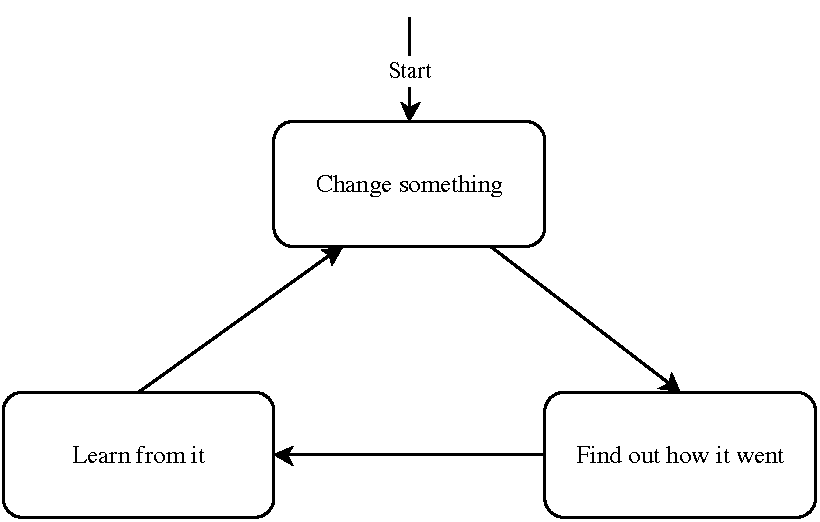
\includegraphics[width=0.9\textwidth]{includes/figures/cycles}
  \caption{Flowchart illustrating the concept of feedback cycles.}
  \label{fig:cycles}
\end{figure}

One way to define feedback cycles is when the results of a process are allowed to influence the process itself. Given that a change has already been introduced, the duration of a feedback cycle can be seen as the time from the moment something is completed (for example, a function is implemented) until the moment we have learned something from it (for example, the function cannot be implemented in this way). Again excluding the actual implementation time, the two actions which then take up time in the feedback cycle include \textit{find out how it went} and \textit{learn from it}. \citep{kniberg2010kanban}

There are software development strategies where we effectively try to reduce the feedback cycle. \Gls{tdd} is one such software development strategy where automated tests are written prior to the development of functional code. This is performed in small, rapid iterations and allows the programmer to execute the tests immediately after the code has been written. \citep[p. 43]{janzen2005test} Here, the development strategy helps to ensure that the feedback cycle time is kept short. 
According to the Agile Alliance\footnote{A non-profit organization promoting agile development principles and practices.}, test-driven development is the following. \citep[p. 44]{janzen2005test}

\begin{quote}
''[Test-driven development is] the craft of producing \textit{automated tests} for production code, and using that process to drive design and programming.''
\end{quote}

The importance of having automated tests relates to the cycle time; if one were to use manual tests, the effort from the developer would be proportional to the number of tests to execute. This practice also assumes that the tests will not be discarded once some code has been written. Instead, the tests are seen as a vital part of the development process, where they can be executed again when new changes are introduced in the system. \citep[pp. 43-44]{janzen2005test} This type of testing is known as \textit{regression testing} \citep[p. 245]{runeson2012regression}. The major downside is that the developer has to maintain both the code and automated tests. \citep{janzen2005test}

\section{Software Testing}
Software testing is done for two main purposes; to judge quality or acceptability and to discover problems. The reason for testing is that we, as humans, know that we are fallible, especially when it comes to software development. People make mistakes or \textit{errors}, resulting in \textit{faults} or representations of errors, which then in turn leads to \textit{failures} in the executing software system. Failures may be more or less apparent to the user; an \textit{incident} is when the user is alerted of the failure. The act of \textit{testing} is to exercise a system with test cases in order to find faults or to show that the software executes correctly. \textit{Test cases}, or simply \textit{tests}, are associated with certain program behaviours, each test case requiring a set of inputs and expected outputs. \citep[pp. 3-4]{jorgensen2002software}

One of the key concepts concerning testing is the level of abstraction. These levels correlate to the traditional software development model, and while this model has its drawbacks, it is useful to identify distinctive levels of testing and clarify the objectives for each level. \citep[pp. 13]{jorgensen2002software} The three traditional levels of testing include \textit{unit testing}, \textit{integration testing}, and \textit{system testing}. For unit testing, the concern is to test software in a unit by unit manner, where a unit is the smallest type of component in the software - for example, a method or function. However, modules can also interact with each other, which opens another possibility for software testing. Integration testing is the idea of testing partial integrations of some modules, and step-by-step include more modules and interactions as testing progresses. System testing then concerns testing for the system as whole, with all its integrations. \citep[pp. 187-188]{jorgensen2002software} Besides these traditional levels there are several other types of testing levels, such as system testing, interaction testing, performance testing, user interface testing, and regression testing, all with different objectives.

Regression testing, which concerns re-testing of modified software, is the level of abstraction that is of focus for the thesis; this type of testing constitutes the majority of software testing efforts in software development. \citep[p. 215]{ammann2008introduction} The terms \textit{regression test suite} and \textit{test suite} will be used interchangeably throughout the thesis. The following section covers various aspects of regression testing in greater detail.

\section{Regression Testing}
For regression testing, one is not concerned with whether the outcome of executing a test can be trusted or not. The previous outcome for each test case defines the correct response; if the test case previously stated that the function was working, it should state so again if run on the system with the new changes, given that the function being tested still passes the test. The focus of regression testing is therefore instead to verify if previously working software still works as specified. The following is the definition of regression testing in the \gls{ieee} standards. \citep[p. 245]{runeson2012regression}
   
\begin{quote}
''[Regression testing is the] selective retesting of a system or component to verify that modifications have not caused unintended effects and that the system or component still complies with its specified requirements.''
\end{quote}

\noindent It is worth noting that in most cases one will have the exact details of the modification of the \gls{sut}, while in some cases such details may not be easily available. For example, when rewriting the system into a new version, such modification details will not be available. \citep[p. 69]{yoo2012regression}

With agile software development practices, focus is on continuous development of software rather than on distinct development phases, as seen in more traditional development methodologies, such as the waterfall development model. As software is being built more often, perhaps several times an hour, regression testing is something which no longer can be run only at the end of a project. \citep[p. 245]{runeson2012regression} Regression tests can be run with every newly introduced change, and when smaller, more frequent changes are introduced, the test cases could potentially be run more often. Even though automated tests are utilized, these will sooner or later consume too much execution time in order for it to be reasonable to run them with every change \citep[p. 245]{runeson2012regression}. If regression tests cannot be run with every change, the feedback cycle time is increased, since the feedback will not be provided until the next time the regression tests are run. The importance of regression testing with every checkin is expressed by \citet[p. 246]{runeson2012regression} in the following statement.

\begin{quote}
''When the regression test suite takes longer than a weekend, the build test suite takes more than overnight, or when the unit test suite takes more than a coffee break — and they do! — there is a need for selecting subsets of test cases in a systematic way, to enable efficient software engineering.''
\end{quote}

\subsection{Testing Techniques}\label{sec:regression-testing-techniques}
Since test suites have the tendency to grow in execution time, to the extent that it prevents efficient software engineering, some type of regression test technique is required in order to shorten the feedback cycle. \citep[p. 245]{runeson2012regression} Many regression testing techniques are using the \gls{pie} model as foundation for their own technique. The \gls{pie} model states that ''a fault can be detected by a test if a faulty statement is executed (E), the execution of the faulty statement infects the state (I), and the infected state (that is, error) propagates to an observable output (P)''. \citep{voas1992pie}

According to a survey by \citet[p. 68]{yoo2012regression}, there are three major types of regression test techniques, namely \textit{test suite minimization}, \textit{test case selection}, and \textit{test case prioritization}; these are discussed separately in the following sections.

\subsubsection{Test Case Selection}
The test case selection techniques aims to reduce the size of a test suite. Most selection techniques are \textit{modification-aware}. This means that the focus is on the identification of which parts of a system that has changed. Test cases are then selected because they are relevant to the introduced changes. Typically, these types of techniques utilize white-box static analysis on the system code. \citep[p. 70]{yoo2012regression} For \textit{regression test case selection} specifically, the aim is to select a subset of tests which are to be used as regression tests. Several types of criteria can be used for evaluating the selection, for example, efficiency and effectiveness (see section~\vref{sec:technique-evaluation}). A test selection technique can be said to be \textit{safe}, which means that no tests are excluded which have the possibility of executing any part of the system that may have been affected by the change. \citep{runeson2012regression}

\subsubsection{Test Suite Minimization}
Utilizing test suite minimization also means that the goal is to reduce the number of test cases by removing redundant test cases. Redundant test cases are defined in terms of code coverage; if a test case covers some part of a program, according to some coverage criterion (for example, method coverage), it is redundant if the same part is also already covered by the rest of the test suite \citep{wong1995effect}. This type of technique is sometimes called \textit{test suite reduction}, implying that the elimination of test cases is permanent. However, minimization and reduction can be used interchangeably, as they essentially are the same. The reason for this is that test suite reduction can produce a temporary test suite, while test suite minimization can produce a test suite which can be used to make permanent changes. \citep[p. 69]{yoo2012regression}

\subsubsection{Test Case Prioritization}
Prioritization of test cases is when test cases are rearranged in an order so that an early maximization of a desired property is achieved. One such property could be fault detection, that is, to detect faults as early as possible. The technique aims to find the optimal permutation in this regard. Selection of test cases is not concerned. The technique also assumes that the test cases can be executed in the permutation it provides. This could be the case if there are dependencies between test cases, so that one test case needs to be run before another. This means that the technique must either take such dependencies into consideration or assume that no such dependencies exist.

\subsection{Technique Evaluation}\label{sec:technique-evaluation}
When introducing regression testing techniques, there is also a need to measure their performance according to some criteria. Depending on which regression testing technique is applied, one could potentially use different evaluation criteria, since the aim of each technique type differs somewhat.

\subsubsection{Test Case Selection}\label{sec:test-cases-selection-metrics}
\citet[p. 529]{rothermel1996analyzing} defined a framework for evaluating regression test case selection techniques. The framework includes four key metrics: \textit{inclusiveness}, \textit{precision}, \textit{efficiency}, and \textit{generality}.

\begin{itemize}
  \item\textit{Inclusiveness} is a measurement of the extent to which the tests will cause the modified system to produce a different output than the original system. A \textit{safe} test selection technique has an inclusiveness of 100\%, which means that all test cases which can reveal different output compared to the original output will be included in the selection.
  \item\textit{Precision} measures the ability of the test selection strategy to avoid selecting test cases which produce the same output for the modified system as for the original system. This can also be described as the ability to exclude test cases which does not reveal faults.
  \item\textit{Efficiency} is a computational cost measurement, in space and time requirements of the test selection technique. This relates to the test selection time, test reduction time, and the test execution time. The measurement measures how practical it is to use the technique.
  \item\textit{Generality} is how well the technique can handle arbitrarily complex modifications in program code, diverse and complex language constructs, and various testing frameworks. In essence, how applicable the technique is in various contexts.
\end{itemize} 	

\subsubsection{Test Suite Minimization}
For the test suite minimization technique, the same framework as for test case selection can be used. However, for minimization, the inclusiveness and precision measurements are not of concern. This is because minimization techniques try to reduce the number of tests while still retaining the same coverage, that is, only eliminating redundant test cases. If only redundant test cases are removed from the test suite, neither of these measurements will be affected. \citep[p. 247]{runeson2012regression}

\subsubsection{Test Case Prioritization}
The aim of a prioritization technique is to order tests according to some evaluation criteria. \citet[pp. 937-938]{rothermel2001prioritizing} defined the Average of the Percentage of Faults Detected (APFD) effectiveness measure in order to evaluate and compare the effectiveness of different prioritization techniques. The measure estimates how quickly faults can be detected by prioritizing test cases. This measure does not include the cost of performing the actual prioritization, as \citeauthor{rothermel2001prioritizing} found it difficult to measure the execution time reliably, and because their implementations were not constructed for efficiency. \citep[p. 247]{runeson2012regression}

\subsection{Researched Techniques}\label{sec:researched-techniques}
Among the different types of techniques, \textit{test case selection} has been the most researched area. The first paper was published by \citet{fischer1997prioritizing} and until the early 1990's, the focus has been on developing effective test selection techniques. \textit{Minimization} techniques were introduced in \citet{harrold1993metholodgy} and \textit{prioritization} techniques were first introduced by \citet{rothermel1999testcase}. The interest in prioritization techniques has been growing ever since, and since 2008 more papers have been published on prioritization techniques than selection techniques. \citep{runeson2012regression}

In an explorative study on \gls{rto}, \citet{anwar2014exploration} set out to find current techniques, tools, mathematical models, objective functions, and sample programs for regression testing. The study covers minimization, prioritization, and selection techniques, which will be covered in the following sections. Selection techniques are covered indirectly, meaning they are usually used alongside a minimization or prioritization technique. A common selection is the tests which execute code that have been modified, in so-called \textit{modification-based} techniques. Note that the term technique is used for all types of techniques relating to \gls{rto}.

\subsubsection{Test Case Prioritization}
The regression test case prioritization techniques presented in the study are presented with their respective authors in table~\vref{tab:prioritization-techniques}. These techniques are described in greater detail below, using the same order as in the table.

\begin{table}[htbp]
  \centering
  \begin{tabular}{|l|l|l|}
    \hline
    \textbf{Authors} & \textbf{Description}\\
    \hline
    \citet{wong1997study} & Minimization \& Prioritization Technique\\
    \hline
    \citet{malhotra2010regression} & Modification-based Prioritization\\
    \hline
    \citet{rothermel1999testcase} & Fault Detection Prioritization Techniques\\
    \hline 
    \citet{mansour2009regression} & C\# Modification-based Prioritization\\
    \hline
  \end{tabular}
  \caption{Researched regression test case prioritization techniques.}
  \label{tab:prioritization-techniques}
\end{table}

\paragraph{Minimization \& Prioritization Technique \citep{wong1997study}} 
The technique first performs a selection of test cases which execute any modified parts of the program. Then a prioritization of these test cases is performed in order to determine the execution order of the tests. Depending on the amount of available resources, for example, time constraints, there is the possibility that not all test cases will be run. However, the test cases given the highest priority will likely have had time to run. This technique combines minimization and prioritization. \citep[p. 264]{wong1997study}

Test suite minimization is performed so that the same coverage is achieved in respect to a certain criterion $\mathcal{C}$ of the original test suite. This means that if the program attribute defined by $\mathcal{C}$ is covered in the original test suite, it will also be covered in the minimized test suite. The minimization is performed on a subset of all test cases, selected using the modification-based technique. This reduces the time needed for the minimization technique, increases the chance of selecting test cases where different output is produced between the old and new systems, and decreases the chance of including redundant test cases. The prioritization technique then orders test cases in increasing order of additional coverage per cost. \citep[p. 265]{wong1997study}

\paragraph{Modification-based Prioritization \citep{malhotra2010regression}}
An alternative modification-based approach was suggested by \citet{malhotra2010regression}. First, test cases are identified which execute modified lines in a system's source code. Next, a prioritization technique is applied that considers which lines have been modified and the total number of modified lines. An execution history over which source code lines each test case executes is kept on record. A deletion algorithm is then applied which updates this history between test executions. The purpose of the deletion algorithm is also to remove redundant tests from the test suite. Tests are seen as redundant if they only cover lines which are covered by other tests. \citep{malhotra2010regression}

\paragraph{Fault Detection Prioritization Techniques \citep{rothermel1999testcase}}
In an empirical study on regression test case prioritization techniques, the authors \citet{rothermel1999testcase} present nine different approaches to prioritize test cases and then evaluate them based on their fault detection rate. These nine approaches are described below. \citep{rothermel1999testcase}

\begin{itemize}
  \item\textit{No prioritization}. Simply used as reference when comparing with other prioritization techniques. This is the application of no technique, the test suite can be considered untreated.
  \item\textit{Random prioritization}. Again, to be used as reference for other prioritization techniques. Test cases are prioritized in some random order.
  \item\textit{Optimal prioritization}. The optimal prioritization is achieved using pre-determined changes and the knowledge of which test cases identify the faults in these changes. This is used as reference in the study and is itself not an actual technique for achieving an optimal prioritization.
  \item\textit{Total branch coverage prioritization}. Determines the total number of decisions, or branches, in a program that were executed by a certain test case, and prioritizes test cases based on this number solely.
  \item\textit{Additional branch coverage prioritization}. An alternative approach to \textit{total branch coverage prioritization} where the technique iteratively selects test cases which yield the greatest branch coverage. After a test case has been selected, branch coverage information is updated, allowing for test cases covering branches which have not yet been covered to be given a higher prioritization.
  \item\textit{Total statement coverage prioritization}. Similar to \textit{total branch coverage prioritization} with the difference that test coverage is defined in terms of program statements, as compared to branches or decisions.
  \item\textit{Additional statement coverage prioritization}. Again, similar to \textit{additional branch coverage prioritization}, except that test coverage is measured in program statements rather than branches. After complete coverage is achieved, there is a need to prioritize the remaining test cases. \citeauthor{rothermel1999testcase} uses \textit{total statement coverage prioritization} in their empirical study for this purpose.
  \item\textit{Total fault-exposing-potential prioritization}. Rather than basing the prioritization purely on coverage, the idea is to try and approximately determine the likelihood that a fault in the covered branch or statement will result in a failure for the test case. This measure is called the \gls{fep} of a test case. Note that in general, faults will not always cause failures; sometimes failures only occur during certain circumstances which might not be covered by test cases. Then, test cases would be prioritized according to some summation of \gls{fep} values for the covered branches or program statements.
  \item\textit{Additional fault-exposing-potential prioritization}. Similar to \textit{total fault-exposing-potential prioritization}, except that previous test case coverage of a program statement is taken into account. In other words, additional executions of a program statement may be less valuable than the first execution.
\end{itemize}

\paragraph{C\# Modification-based Prioritization \citep{mansour2009regression}}
The technique is based on three phases, where the first phase constructs an \gls{acd}, which consists of the classes that were affected by the introduced change in the system's source code. The second phase constructs a \gls{cig} from the \gls{acd}, effectively reducing the amount of test cases for the third phase. The third phase further reduces the amount of tests and prioritizes the remaining test cases. Reduction is done by, for each affected method, randomly selecting a test case which covers the method. Prioritization is done by either executing (1) test cases which needs to be retested that cover classes in the \gls{acd} or (2) test cases which run affected execution paths leading to the modified code. It is left up to the tester to select either one or both of these alternatives, and in which order to run them. \citep{mansour2009regression}

\subsubsection{Test Suite Minimization}
The regression test suite minimization techniques presented in the study are given with their respective authors in table~\vref{tab:minimization-techniques}. Note that there is an overlap with the first prioritization technique in table~\ref{tab:prioritization-techniques}, since the technique uses both prioritization and minimization approaches. Except for the overlapping technique, all other minimization techniques are described in greater detail below, in the order they are presented in the table.

\begin{table}[htbp]
  \centering
  \begin{tabular}{|l|l|l|}
    \hline
    \textbf{Authors} & \textbf{Description}\\
    \hline
    \citeauthor{wong1997study} & Minimization \& Prioritization Technique\\
    \hline
    \citeauthor{sivaprasad2011efficient} & Coverage Data using Data-flow Analysis\\
    \hline
    \citeauthor{orso2004scaling} & Code Partitioning \& Selection Technique\\
    \hline
    \citeauthor{nanda2011regression} & Non-code Regression Testing Technique\\
    \hline
    \citeauthor{chittimalli2009recomputing} & Re-computation of Coverage Data\\
    \hline
    \citeauthor{willmor2005safe} & Modification-revealing Tests for Databases\\
    \hline
    \citeauthor{sun2011constraint} & Constraint-based Test Suite Minimization\\
    \hline
    \citeauthor{prasad2012optimizer} & Hierarchal Clustering of Similar Test Cases\\
    \hline
    \citeauthor{parsa2010optimization} & Minimal Overlap in Requirements Coverage\\
    \hline
  \end{tabular}
  \caption{Researched regression test suite minimization techniques.}
  \label{tab:minimization-techniques}
\end{table}

\paragraph{Coverage Data using Data-flow Analysis \citep{sivaprasad2011efficient}}
The idea for this technique is to compute coverage data for two or more versions of the same software and use the differences in coverage as a basis for minimization. The technique is described as a three step process, where the first step is to identify the program components for which to compute coverage data. The second step is to apply execution tracing and data-flow analysis on the identified program components. The data-flow analysis is used to collect information about how variables are used and defined. The data-flow analysis is dynamic, meaning that the program is executed in order to perform the analysis. From this analysis, it is possible to identify paths which satisfy some selected coverage criteria (for example, statement coverage, method coverage, call coverage, and condition coverage). The third step is to repeat this for another version, where changes have been introduced, to identify changed entities, and select relevant test cases. \citep{sivaprasad2011efficient} 

\paragraph{Code Partitioning \& Selection Technique \citep{orso2004scaling}}
The developed technique is an algorithm for software written in the Java language, although it can be adapted to work for other object-oriented languages. The algorithm can handle the object-oriented features of the language and is both safe and precise. The technique consists of two parts: partioning and selection. The partitioning part constructs a high-level Interclass Relation Graph (IRG) over the original system and the modified system. Each of these graphs is a representation of inheritances and usages among modules in the system. A quick analysis is applied on the graph in order to determine which parts of the system to analyze in greater detail. The selection part constructs a more detailed graph of the identified components in the first part and analyzes these graphs to find differences between the two systems. Test cases are then selected based on whether they traverse the changes or not. A prototype tool, DejaVOO, that implements the technique was presented as part of the research. \citep{orso2004scaling}

\paragraph{Non-code Regression Testing Technique \citep{nanda2011regression}}
According to \citet{nanda2011regression}, most existing techniques focuses on changes to code components, and completely ignores non-code elements, like configuration files and databases, which can affect the behaviour of the system. The presented technique allows to select tests which take into account changes to non-code elements. The idea is to compute traceability between test cases and the externally provided data, which is accessed by the system. The technique models property files, or essentially configuration files, as \textit{(key, value)} pairs. Databases are modeled as a set of tables, where for each table some information is stored, like the primary key, column names, whether the value can be null, the actual value, etc. Using the models, a difference analysis can be performed to find changes in external components. \citep{nanda2011regression}

Traceability between test cases is assumed to be present, that is, it is possible to determine which properties are accessed by a certain test case. This can for example be done by code instrumentation on the specific \gls{api} used for handling properties. For databases, \gls{sql} queries are to be traced during execution. Depending on the \gls{api} used for accessing databases, it might prove easy to perform this kind of tracing. \citep{nanda2011regression}

By utilizing the traceability between test cases and a differential analysis to find changed external components, one can perform test selection so that test cases covering these components are selected. \citep{nanda2011regression}

\paragraph{Re-computation of Coverage Data \citep{chittimalli2009recomputing}}
The technique helps in computing updated coverage data for an existing test selection algorithm. The technique does not require rerunning any test cases that do not cover changed statements from the previous version to the current one. This means that there is no need to rerun an entire test suite and that there is no need to approximately estimate coverage data, or reuse existing outdated coverage information. \citep{chittimalli2009recomputing}

\paragraph{Modification-revealing Tests for Databases \citep{willmor2005safe}}
Proposes a new definition of \textit{safe} regression test selection algorithms, taking into account interactions with database state. It is important to take into account the existing database state if the test is performing database operations. \citep{willmor2005safe}

\paragraph{Constraint-based Test Suite Minimization \citep{sun2011constraint}}
Presents a constraint-based test suite minimization technique, where test constraints are used in order to reduce the number of test cases. A test constraint is defined to be the conditions which are necessary for a certain bug to be detected. To see if a test case can detect a bug, it is necessary to check whether the test constraints are fulfilled by the test case. Test constraints can be computed using program analysis techniques. Selection and reduction is then based on when tests satisfy the constraints. When all constraint conditions are satisfied by the selected tests, the process is completed. Since the test constraints can be determined using program analysis, there is no need to run the program. \citep{sun2011constraint}

\paragraph{Hierarchal Clustering of Similar Test Cases \citep{prasad2012optimizer}}
The technique is a five step approach. The first step is to create a mapping of test cases to functions which are executed when the test cases are called, respectively. Then, hierarchical clustering is used to group similar test cases. Within these clusters, sequences of function calls are retrieved and used in later comparisons. The fourth step is to compare line coverage of tests, and the final step performs comparisons on branch coverage. These comparisons enable the ability to find and remove redundant tests from the test suite. \citep{prasad2012optimizer}

\paragraph{Minimal Overlap in Requirements Coverage \citep{parsa2010optimization}}
Proposes a greedy algorithm that attempts to select test cases so that the maximum number of testing requirements are satisfied. Testing requirements are software requirements to which test cases have been mapped. The goal is at the same time to have a minimal overlap in requirements coverage with the other test cases in the test suite. By matching the maximum number of testing requirements, the goal is to select test cases which are effective at fault detection. By reducing the overlap in requirements coverage, an attempt is made to remove redundant test cases from the test suite and to select unique test cases in regard to requirements coverage. These attempts try to increase the fault detection effectiveness. \citep{parsa2010optimization}

\subsection{Current Testing Practice}
\citet{engstrom2010qualitative} performed a qualitative survey on industry regression testing practices. For the survey, focus group discussions and a questionnaire for verification were utilized in a \gls{spin}. Definitions, practices, challenges, and improvements of regression testing were discussed with the groups. In total, 46 software engineers from 38 different organizations participated in the survey. Some of the results from this study is presented in the following sections. \citep[p. 248-249]{runeson2012regression}

\subsubsection{Definition}
Regression testing was seen as the process of repetitively running tests in order to verify that previously working software still works after other parts have been modified. The goal of regression testing could differ; sometimes it was used as a measure of quality of the software, sometimes it was used to find defects, and it was also used for deciding what would be prioritized in the future of a project. Changes which would initiate regression testing included ''new versions, new configurations, corrections, changed solutions, new hardware, new platforms, new designs, and new interfaces''. Amount and frequency was determined by several factors, including ''risk, the amount of new functionality, the amount of fixes, and the amount of available resources''. \citep[p. 249]{runeson2012regression}

\subsubsection{Application}
Regression testing occurs at various different levels, for example, module, component, and system levels. It was also conducted during different stages of the development process. Some applied it as early as possible, some as late as possible, and some claimed to be using it continuously throughout the development process. Early regression testing can be used with the aim to find defects early, while late regression testing may be used for approval purposes. How often regression testing occurs also varies between organizations, everywhere from daily to only at specific milestones. \citep[p. 249]{runeson2012regression}

\subsubsection{Techniques}
The method to use for selecting test cases for regression testing varied between organizations. Sometimes tests were selected from the developer's suite and sometimes from the tester's suite. In some cases, tests were selected from a regression test suite, and in some cases new regression tests were designed. The regression test techniques also varied, from executing every regression test case, to combine static and dynamic selection, to complete retest of critical parts, and to concentrate the efforts on the introduced changes. Other techniques included ad hoc selection, smoke test (testing with a subset of all test cases to cover the most important functionality), prioritization and then running as many test cases as feasible, and focusing the testing efforts on functional test cases. Both manual and automatic regression testing were found to be used. \citep[p. 250]{runeson2012regression}

\subsubsection{Problems}
From an open discussion in the focus group, the following several major weaknesses and strengths were identified. Some of the identified problems were very common, while some others were specific to certain organizations. \citep[pp. 250-251]{runeson2012regression}

For \textit{test case selection}, it was stated to be difficult to understand the impact of changes to existing code and from that make a selection. Prioritizing test cases based on product risks and fault detection rate, and being confident that no critical faults had been missed were all seen as problems. Deciding how many tests to select and assessing the test coverage was also viewed as problematic. Worth noting is that no references to researched regression testing techniques were mentioned.

When \textit{designing test cases}, most participants stated that there was a lack of time and resources for regression testing. One suggestion that was brought up was to focus on test-driven development, and include the written tests in the regression test suite.

\textit{Automated testing} causes problems in terms of implementation, maintenance of test suites, and often manual analysis of results. Manual testing was viewed as time and resource consuming.

Certain \textit{problematic areas} were identified that was said to be specific for regression testing. These included testing in a real target environment, as well as a simulated target environment, regression testing third party products, and the testing of user interfaces.

Participants were unsatisfied with the \textit{presentation and analysis of test results}. The reporting was said to many times be inconsistent and often there was no time to do a more thorough analysis.

The \textit{maintenance} of test suites was seen as a problem, where it was difficult to trace regression tests to requirements. It was also a problem that some regression tests could be seen as redundant in terms of test coverage.

The amount of dependencies and modularity of the design was said to be related to the \textit{testability} of the system. Designs where it is simple to separate tests for different parts was sought after. There was a stated need for testability design guidelines, software modularization, and clearer dependencies.

\subsubsection{Conclusions}
According to the survey, the industry practice on regression testing is mostly based solely on experience and specifically not on any systematic approaches. Researchers therefore better need to understand the needs in the industry and on the used practices. This is captured by \citet{rooksby2009testing} in their writings on real world testing practices; ''improvements in industry are not always sophisticated and accurate as is often pursued in research''. \citep[p. 251]{runeson2012regression}

\subsection{Receiving Early Feedback}\label{sec:receiving-early-feedback}
In relation to feedback cycles, as presented in section~\vref{sec:feedback-cycles-concept}, the importance of receiving early feedback should not be underestimated. In the survey by \citet{yoo2012regression}, the authors state that ''existing empirical studies show that the application of these [regression testing] techniques can be cost-effective''. In an empirical study on time constraints on the cost-benefits of regression testing, \citet{do2008empirical} studied six different regression test techniques, while considering four different time constraints taking up 25\%, 50\%, 75\%, and 100\% of the total test execution time, respectively. The different prioritization techniques were evaluated under each of these constraints using a cost-benefit model. From the results of the study, the authors conclude that despite the time constraints affecting the prioritization techniques, it was always beneficial to use a test case prioritization technique from a cost-benefit perspective. \citep[p. 93]{yoo2012regression}

\section{Continuous Integration}
As described in section \vref{sec:agile-software-development}, agile development strategies strive to integrate modules and components continuously throughout the development of a system. An interesting question is whether in a real project, are there any people actually interested in running the system or not? The developers may commit new changes to the version control system and even run automated tests, but may never actually run the whole system. Since it is of interest to have a working system at all times, or at least as often as seen realistically, should one not actually run the system to be sure that the components have integrated properly? \Gls{ci} is the idea that with every change that is introduced, the entire system is built and run, while automated tests are being run against it. \citep[p. 55]{humble2010continuous} Together, \citet{humble2010continuous} describe their experiences with continuous integration, comparing it with projects where it is not used.

\begin{quote}
  ''[...] we have seen projects that spend at most a few minutes in a state where their application is not working with the latest changes. The difference is the use of continuous integration.''
\end{quote}

When not using continuous integration, the software can be seen as broken until someone proves different. When a change is introduced into the system, how do one know that the system still works? Normally, faults would be detected during an integration process or during testing. When using continuous integration, the system is setup and proven working with every committed change to a version control system. This assumes that the suite of automated tests is sufficient to, in a sense, prove that the system works as intended. \citep[p. 56]{humble2010continuous}

In a basic continuous integration model, there are two components which must exists. First of all, there needs to be a version control repository. Basically, all files related to the project and which are required in order to build, install, run, and test the system (code, tests, scripts, etc.) should be in the version control system. The other component is the possibility of starting an automatic build. It can range from something so simple as compiling the source code and running the automated tests, to setting up complex distributed environments. Apart from this, there also needs to be an agreement within the development team to use continuous integration; it is a practice, not a tool. \citep[pp. 56-57]{humble2010continuous}

\subsection{Development Workflow}
A basic continuous integration system contains a server which performs the automatic build and executes automated tests. There are several open source and commercial softwares available on the market which provides this kind of functionality. Jenkins (formerly Hudson) and CruiseControl.rb are examples of two open source system, while Go from ThoughtWorks Studios and TeamCity from JetBrains are two commercial alternatives. With such a server software in place, the typical development workflow with continuous integration would look something like that in figure~\vref{fig:workflow}. Assuming that a change has been made, the process can also be described according to the following steps. \citep[pp. 58-59]{humble2010continuous}

\begin{enumerate}
  \item Check whether a build is currently running on the continuous integration server; if so, wait while it finishes. If the build is not passing, assist in fixing the issue at hand.
  \item When the build passes, get changes from the version control system.
  \item\label{itm:local-build-test} Run the build script and the automated tests. If the local build does not pass the tests, fix the issue at hand.
  \item When the build passes, push changes to the version control system.
  \item Wait as the \gls{ci} system initiates and runs a build with your changes.
  \item If the build does not pass, fix the issue at hand, and go back to step~\ref{itm:local-build-test}.
  \item If the build passes, continue by moving on to the next task.
\end{enumerate}

\begin{figure}[htbp]
  \centering
  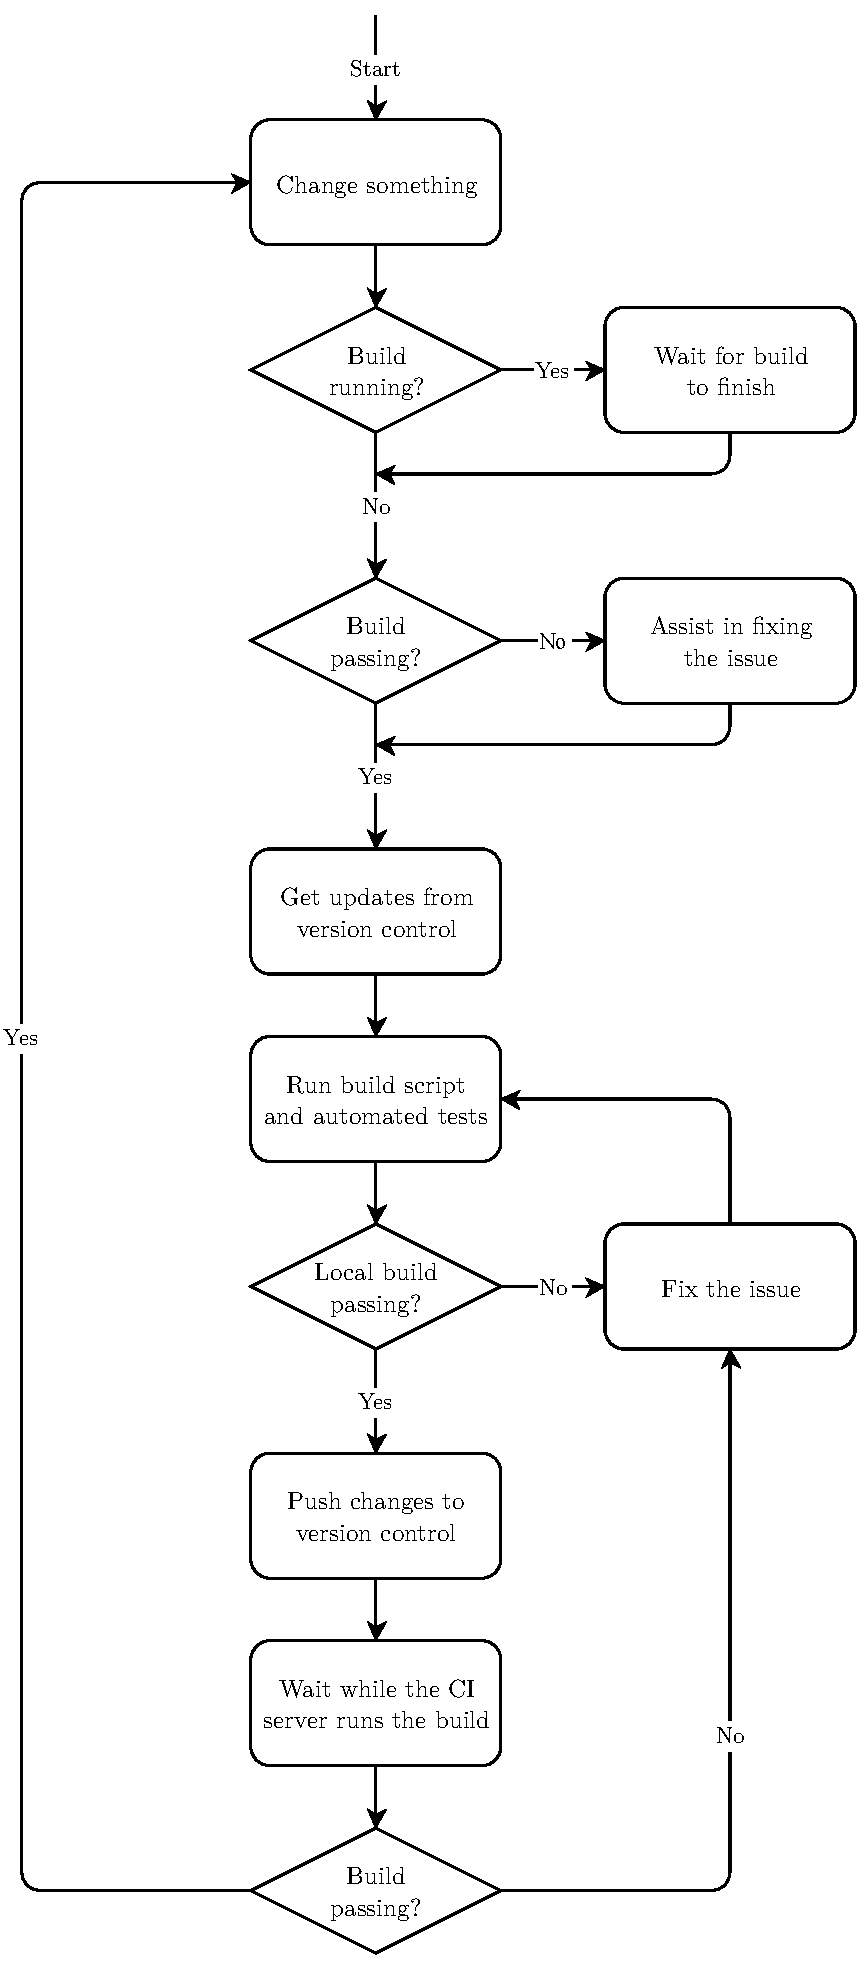
\includegraphics[height=0.95\textheight]{includes/figures/workflow}
  \caption{Typical development workflow with continuous integration.}
  \label{fig:workflow}
\end{figure}

\subsection{Testing Feedback Cycles}
When working in an environment with continuous integration, similar to the workflow described in the previous section, there are two types of feedback cycles which relate to software testing. The first such cycle is the one where the developer makes a change, runs the automated tests and takes part of the results, and learns from it. If the tests did not succeed, the developer can continue to make changes to the system or tests until the tests pass.

The second feedback cycle starts with pushing changes to the version control system. In this case, the continuous integration system will build, start, and test the system --- perhaps executing a more extensive set of test cases than what the developer did on his local build. The developer can take part of test results as tests are being executed by the continuous integration system and learn from the status of the executed test cases.

\chapter{Implementation}\label{chap:implementation}
This chapter describes the implementation of a regression testing technique. First, a description of the project context is given, along with current testing approach and perceived problems. Section~\ref{sec:technique-implementation} then continues by describing the selection process of a researched regression technique and the implementation details of the selected technique.

\section{Project Description}\label{sec:project-description}
This section describes the project context of the thesis. The following section gives a brief overview of the project. In section~\ref{sec:testing-approach}, an overview of the current test setup is provided, followed by the perceived problems with the setup in section~\ref{sec:perceived-problems}. Section~\ref{sec:interview-testing-techniques} then briefly presents existing knowledge of researched regression testing techniques. Finally, the feedback cycle times of the project are considered in section~\ref{sec:project-cycle-times}.

\subsection{Project Overview}
The project context concerns a joint website for healthcare in Sweden, including advice, information, and electronic services. The project has been in active development for about four consecutive years, employing around four to six developers working full time. Agile software development practices have been used in the project, with influences from Scrum, \gls{xp}, and \gls{tdd}. The adoption of \gls{tdd} becomes apparent when examining the project's source code; the project currently contains more than 50,000 lines of code, out of which approximately 40\% is test-related source code. The project is being actively developed, so these figures will change.

Development is performed in the Visual Studio 2012 \gls{ide}, with the ReSharper extension, using the C\# programming language. \Gls{iis} is used as web server, together with the \gls{sql} Server 2008 database system and EpiServer CMS 6 R2 for managing content. The Asp.Net MVC 3 framework is used for the web application and project dependencies are managed using the NuGet package manager integrated with Visual Studio. For distributed version control, Git is used in conjunction with GitHub.

\subsection{Testing Approach}\label{sec:testing-approach}
The project employs a continuous integration system, namely Jenkins, with a similar workflow to the one depicted in figure~\vref{fig:workflow}. As committed changes in Git are pushed to the central GitHub repository, Jenkins notices the change and compiles the software, runs automated tests, and deploys the latest version. Developers make sure that newly created tests, for the code they write, passes before changes are pushed to the GitHub repository. There are several different types of tests utilized in the project; the following sections discusses each of these types separately. How these different types of tests are used for regression testing is described for each individual type. Not described below are \textit{performance testing} and \textit{manual testing} which are are not in the scope of the thesis but used in the project to some degree.
\subsubsection{Unit Testing}
In the project context, unit testing is used as a way to test individual modules and methods. The syntax of the NUnit\footnote{Unit testing framework, see \url{http://www.nunit.org/}.} framework is used in order to write test cases and the included runner is used for executing tests. For mocking module dependencies, the RhinoMock framework is utilized. Unit tests are primarily written as part of \gls{tdd} efforts, before the actual implementation has been developed. When developing new functionality, developers should ensure that the unit tests are passing before changes are committed to the version control system. The unit test cases are reused as part of regression testing and are run by the continuous integration system with every commit. As there are several thousand unit test cases, the execution time is a couple of minutes on both developers' machines and on the system running Jenkins.

\subsubsection{Integration Testing}
Integration tests are used to test interactions between system components in the project. This is done by interacting with a web browser which navigates around the website while interacting with page elements and checking that the expected elements are visible. These tests are written using Selenium\footnote{Web browser automation framework, see \url{http://seleniumhq.org/}.}, which is a browser automation framework. This has been coupled with PhantomJS\footnote{Headless web browser engine, see \url{http://phantomjs.org/}.} - a headless full web stack browser. As with unit tests, integration tests are written using NUnit and executed using its runner. These tests are reused for regression testing by re-executing some of them with every commit and others nightly with a certain periodicity.

\subsubsection{User Interface Testing}
Graphical user interface tests are used to tests interactions flows (possible ways to navigate around the interface) in the project. The tests are not written in C\#, as for the unit and integration tests, but instead in Capybara\footnote{Acceptance test framework, see \url{http://jnicklas.github.io/capybara/}.}, in the Ruby programming language. The Cucumber\footnote{Behavior driven development framework, see \url{http://cukes.info/}.} framework is used to write tests, where acceptance tests are written in plain text and translated into test cases using step definitions. Some of these tests are run with PhantomJS, as for the integration tests, while some are run in the latest version of the Firefox web browser. For regression testing, some tests are re-run with a certain periodicity and some are run with every commit. Tests with very long execution time have been identified and have been set to run with a longer time between executions, running them more seldom. Before releasing a new version of the software, developers must make sure that all user interface tests are passing.

\subsection{Perceived Problems}\label{sec:perceived-problems}
During a meeting on 24 April 2014 with one of the software developers working in the project, there was stated to be some perceived problems with unit testing. While developers make sure that new unit tests are passing for their new changes, existing unit tests may not always be re-run due to the long execution time. The same developer stated that it would be desirable to reduce the execution time of the unit tests for the reason of not having second thoughts on running all unit tests before committing changes.

According to an interview conducted with a software developer on 13 May 2014, the main problem with the current test setup was the execution time, which was also said to be the general opinion of the developers in the project. While the test case coverage was stated to be relatively good, the problem concerned the execution time of integration tests and user interface tests. Current efforts have included to rewrite tests to execute faster and to evaluate new frameworks and tools, such as SauceLabs for having a cloud testing platform. Suggested improvements were to have execution time in mind when developing new test cases and to execute tests in parallel in order to decrease the execution time. The respondent noted that parallelization could prove difficult if there are dependencies between test cases; something which was believed to not be the case for the project.

The problem with having a long execution time, according to the respondent, was that there can be hidden faults in the software, due to the test cases not being run, and therefore possibly not revealing faults. The concept of feedback cycles was mentioned briefly, where it was seen as a benefit to have a shorter feedback cycle by shortening the total execution time of the test suites. (Anonymous, 2014, Interview with Software Developer, 13 May)

\subsection{Testing Techniques}\label{sec:interview-testing-techniques}
For \textit{test case selection}, the respondent did not seem to have any knowledge of the regression test case selection techniques presented in existing research, as presented in section~\ref{sec:researched-techniques}. However, the idea of selecting test cases was familiar, and the benefits of performing selection was stated to be to ''find faults faster by executing tests that execute quickly more often''. To be noted is that the statement related to selecting some regression tests cases for execution with every commit, as was the case with integration tests and user interface tests. In other words, the respondent was referring to another way of selecting test cases compared to the ones presented in research. (Anonymous, 2014, Interview with Software Developer, 13 May)

Regarding \textit{test case prioritization}, the respondent did not seem to be aware of any prioritization techniques as seen in existing research. Some customer perspective, or business value perspective, was suggested to be used as foundation for prioritization. However, the respondent was referring to priority as in increasing the effort on improving such test cases. When asked about the benefits of prioritization as changing the execution order of the test cases, the respondent could not see why that would be beneficial, as all tests cases would be executed anyway. (Anonymous, 2014, Interview with Software Developer, 13 May)

\subsection{Feedback Cycle Times}\label{sec:project-cycle-times}
For the feedback cycle times, we are interested in determining the time it takes to receive feedback on introduced changes. Let us first consider the case of unit testing. Regression unit tests are executed on the continuous integration system with every commit. When executing test cases, they are run in no guaranteed order\footnote{Previously, in versions 2.5 or earlier, tests were executed in alphabetical order. This changed in later versions, and test cases are now executed as they are discovered by NUnit. \citep{poole2012test}}. NUnit does not currently support parallel execution of test cases, so tests are executed sequentially by a single thread \citep{poole2013parallel}. 

Essentially, we have no information about which order failing test cases will be executed. Therefore, the feedback cycle times can only be estimated using example scenarios and estimates. The same applies for integration testing, which is also written and executed using the NUnit framework. The exception here is that there is a subset of all test cases being run with every commit, while the rest of the tests are run with a certain periodicity. The thesis does not focus on the Ruby programming language; user interface testing will therefore not be considered further.

For the purpose of evaluation, the following sections introduce some notation and reason about the current test setup. First, the notation used in the thesis is presented, after which unit testing is considered. Finally, the differences with integration testing are discussed. The notation is then used in section~\vref{sec:theoretical-improvements} where the improvements of the implemented technique are considered. An evaluation of the implementation in the project context is provided in section~\vref{sec:integration-evaluation}.

\subsubsection{Notation}
A set of $n$ test cases ordered by execution order is denoted $T = \langle T_1,\ldots,T_n \rangle$. This means that test cases are executed starting with $T_1, T_2, \ldots, $ and $T_n$ is executed last. The order can be either with or without a prioritization technique in effect. All normal set operations are used on these ordered sets of test cases. We let $E(T_i)$ denote the execution time of test case $T_i \in T$. Also, when discussing prioritization techniques, we let $W(T_i)$ denote the weight assigned to test case $T_i \in T$. A higher weight means that the test case is executed earlier, that is, $W(T_i) \geq W(T_{i+1})$, $\forall\, T_i, T_{i+1} \in T$.

\subsubsection{Single Failing Test Case}
On a theoretical level, we could assume that the test cases are being executed on a discrete uniform distribution basis. Given an execution order of the test cases, $T = \langle T_1,\ldots,T_n \rangle$ where $n$ is the number of test cases, the following can be said for a failing test case $T_f \in \langle T_1,\ldots,T_n \rangle$, $1 \leq f \leq n$.

\begin{itemize}
  \item In the \textit{best case}, $T_f$ will be executed first; $f = 1$.
  \item In the \textit{average case}, $T_f$ will be executed in the middle; $f = n/2$.
  \item In the \textit{worst case}, $T_f$ will be executed last; $f = n$.
\end{itemize}

Let $E(T_i)$ denote the execution time of test case $T_i \in T$, then the time for feedback from the failing test case $T_f$ is $\sum_{i=1}^{f}E(T_i)$. In other words, we have to execute all preceding test cases and the failing test case in order to receive feedback. In this case, the feedback cycle time can be reduced by running the failing test as early as possible. So, in the cases above we have the following results regarding the feedback cycle times.

\begin{itemize}
  \item In the \textit{best case}, the feedback cycle time is $E(T_1)=E(T_f)$.
  \item In the \textit{average case}, the feedback cycle time is $\sum_{i=1}^{n/2}E(T_i)$.
  \item In the \textit{worst case}, the feedback cycle time is $\sum_{i=1}^{n}E(T_i)$.
\end{itemize}

For passing tests, we have to execute all the tests in order to know that they are indeed passing, so this feedback time is equal to the sum of the execution time of all test cases, that is $\sum_{i=1}^{n}E(T_i)$.

\subsubsection{Multiple Failing Test Cases}
In reality there may be more than one failing test case; let $F = \langle T_{f_1},\ldots,T_{f_m} \rangle$ denote the set of failing test cases, where $m$ is the number of failing test cases, $0 \leq m \leq n$, $1 \leq f_i \leq n$ for $1 \leq i \leq m$. Also, let $F$ keep the ordering from $T$, so that $f_1 < \ldots < f_{i-1} < f_i < f_{i+1} < \ldots < f_m$, $\forall\,T_{f_i} \in F$.

When having several failing test cases, there are multiple ways to evaluate the feedback cycle time. For failing test cases we are interested in knowing that they are failing as soon as possible. One way to evaluate this would be to consider the time for the first $1 \leq k \leq m$ failing test cases to execute, which is calculated as $\sum_{i=1}^{f_k} E(T_i)$. Using the same best, average, and worst case as for a single failing test case, the following can be said.

\begin{itemize}
  \item In the \textit{best case}, all failing test cases are executed first, so we only have to execute the failing test cases. The feedback cycle time is $\sum_{i=1}^{k}E(T_i)$. 
  \item In the \textit{average case}, the $0 \leq k \leq m$ failing test cases should be within the first $\ceil{\frac{kn}{m}}$ test cases. The average feedback time is $\sum_{i=1}^{\ceil{\frac{kn}{m}}}E(T_i)$.
  \item In the \textit{worst case}, all failing test cases are executed last, so we have to execute almost all the tests. The feedback cycle time is $\sum_{i=1}^{n-m+k} E(T_i)$.
\end{itemize}

For passing test cases, we again need to execute all tests, as for the case of a single failing test case. The time required for this is once more $\sum_{i=1}^{n}E(T_i)$.

\subsubsection{Integration Testing Differences}
As previously stated, the differences between unit testing and integration testing is that a subset of all test cases are being run with every commit, while the rest of the tests are run with a certain periodicity. Given an ordering of all integration tests, $T$, we let the first $1 \leq c \leq n$ test cases be run with every commit, so that $T=\langle T_1, \ldots, T_c \rangle\cup\langle T_{c+1},\ldots,T_{n} \rangle$, assuming that the original ordering in $T$ is kept. It is then possible to treat these two parts as have been described for unit testing. For the second part, we also have to include the time until the next run of the tests in the feedback cycle time.

\section{Technique Implementation}\label{sec:technique-implementation}
In this section, the implementation of a researched regression testing technique is described. The following section describes the process of selecting a suitable technique. Section~\ref{sec:technique-description} then continues to describe the selected technique in greater detail. An overview of the implemented technique is given in section~\ref{sec:implementation-overview}, while the implementation details are covered in section~\ref{sec:implementation-details}.

\subsection{Technique Selection}
In the existing research on regression testing, as presented in section \vref{sec:researched-techniques}, there exists a total of 12 unique papers, each one presenting a different technique for regression test case prioritization or test suite minimization. Out of these 12 techniques, eight of them are for regression test suite minimization, which is out of the scope for implementation in the thesis. Left is four techniques for regression test case prioritization. Among these four techniques, one is to be selected as reference for the implementation. The following four criteria are used in order to evaluate the techniques.

\begin{enumerate}[label=EC.\arabic*]
  \item\label{itm:ec:suitability-project} \textit{Suitability for the project context}. An estimate of how suitable a regression testing technique is for the project context. If the technique is specific to technologies utilized in the project, this is preferred to techniques for other technologies. Underlying assumptions for the techniques could also potentially reduce the suitability for the project.
  \item\label{itm:ec:realization-potential} \textit{Implementation realization potential}. This is an estimation of how realistic it is seen to implement the regression testing technique. The evaluation criteria takes into account several factors, such as implementation details and the level of detail for algorithm descriptions.
  \item\label{itm:ec:partial-implementation} \textit{Partial implementation ability}. Regression testing techniques usually consist of several steps, together forming an algorithm describing the technique. If a technique helps in solving the thesis problem by only implementing some of the initial steps, this would be preferable due to the limited time frame of the thesis work.
  \item\label{itm:ec:cycle-time} \textit{Potential for reducing feedback cycle times}. As there are several ways to reduce feedback cycle times, techniques which could reduce the feedback cycle time more than other techniques are preferred. For example, a technique using both selection and prioritization could potentially reduce the feedback cycle time more than a technique only performing a selection of test cases without prioritizing tests. Inclusiveness, precision, and efficiency metrics are relevant for selection techniques, while, for example, the APFD measurements are relevant for prioritization techniques. Section~\vref{sec:test-cases-selection-metrics} has information on these metrics.
\end{enumerate}

Following are the evaluations for each of the test case prioritization techniques, according to the four evaluation criteria. For each evaluation criteria, a grade is given on a scale from 1 to 5, where a higher score is more preferable than a lower score. The results of the evaluations are summarized in table~\ref{tab:technique-evaluation}, along with the total sum of the grades for each technique. All of the evaluation criteria are weighted equally when calculating the total sum.

\begin{table}[htbp]
  \centering
  \begin{tabular}{|l|c|c|c|c|c|}
    \hline
      \textbf{Technique / Evaluation} & \textbf{\ref{itm:ec:suitability-project}} & \textbf{\ref{itm:ec:realization-potential}} & \textbf{\ref{itm:ec:partial-implementation}} & \textbf{\ref{itm:ec:cycle-time}} & \textbf{Total}\\
      \hline
      \citet{wong1997study} & 3 & 1 & 5 & 3 & 12 \\
      \hline
      \citet{malhotra2010regression} & 1 & 2 & 5 & 1 & 9 \\
      \hline
      \citet{rothermel1999testcase} & 3 & 1 & 1 & 2 & 7 \\
      \hline
      \citet{mansour2009regression} & 4 & 4 & 5 & 5 & 18 \\
    \hline
  \end{tabular}
  \caption{Summary of the test case prioritization technique evaluations.}
  \label{tab:technique-evaluation}
\end{table}

\paragraph{Minimization \& Prioritization Technique \citep{wong1997study}}
Constraints or assumptions that would prevent the technique from not being suitable for the project are not present, but the paper lacks in algorithm details and is therefore not suitable for implementation ($\text{\ref{itm:ec:suitability-project}} = 3$, $\text{\ref{itm:ec:realization-potential}} = 1$). Selection and prioritization can be applied in different steps, allowing for partial implementations ($\text{\ref{itm:ec:partial-implementation}} = 5$). Both modification-based selection and minimization or prioritization techniques are utilized, which gives a good potential for reducing feedback cycle times. However, the case study reveals very varying rates of precision and inclusiveness ($\text{\ref{itm:ec:cycle-time}} = 3$).
 
\paragraph{Modification-based Prioritization \citep{malhotra2010regression}}
The algorithm descriptions seem to be on a low detail level but the algorithm uses the line numbers of the modified lines of source code, which is seen as major constraint for both suitability for the project and implementation potential. This is because changes will rarely only be line modifications and directly examining source code is not desirable ($\text{\ref{itm:ec:suitability-project}} = 1$, $\text{\ref{itm:ec:realization-potential}} = 2$). Selection and prioritization can be applied in different steps, allowing for partial implementations ($\text{\ref{itm:ec:partial-implementation}} = 5$). Both modification-based selection and prioritization techniques are utilized, which gives a good potential for reducing feedback cycle times. However, no empirical evaluation is given ($\text{\ref{itm:ec:cycle-time}} = 1$).

\paragraph{Fault Detection Prioritization Techniques \citep{rothermel1999testcase}}
There does not seem to be any apparent constraints or assumptions which prevents an implementation for the project context ($\text{\ref{itm:ec:suitability-project}} = 3$). However, no detailed algorithms are presented, only brief descriptions, so implementation potential is seen limited and therefore also the partial implementation ability ($\text{\ref{itm:ec:realization-potential}} = 1$, $\text{\ref{itm:ec:partial-implementation}} = 1$). Only prioritization techniques are considered in the paper, excluding potential selection techniques. This is the only paper where the APFD measurement is used, so it proves difficult to compare it to other prioritization techniques ($\text{\ref{itm:ec:cycle-time}} = 2$).

\paragraph{C\# Modification-based Prioritization \citep{mansour2009regression}}
The technique is specifically designed for the C\# programming language, taking into account its specific language constructs. Since C\# is used in the project context, this is seen as very favourable if considering unit tests and integration tests ($\text{\ref{itm:ec:suitability-project}} = 4$). The technique assumes that the changed and deleted methods between two versions of a program can be detected and that test coverage information is available, that is, a mapping of test cases to methods which are executed during the test. Some code analysis in the form of class diagram generation for finding base classes is also required. Algorithm details are provided and seems to be reasonably clear enough to understand for implementation purposes ($\text{\ref{itm:ec:realization-potential}} = 4$). The technique consists of three phases, including several types of selection and prioritization. Only implementing the first phases would help in solving the thesis problem, while the second and third step could be seen as an improvements ($\text{\ref{itm:ec:partial-implementation}} = 5$) After applying the first and second phase, the inclusiveness is still 100\%, while precision is in the 94-100\% range. Applying the final phase reduces the inclusiveness to around 25\% but maintains a precision of 100\%. This allows for prioritizing which measurement is seen as most important. The three phases combined uses both selection and prioritization ($\text{\ref{itm:ec:cycle-time}} = 5$).

\subsection{Technique Description}\label{sec:technique-description}
From the evaluation in the previous section, it seems like the modification-based prioritization for C\# by \citet{mansour2009regression} is most suitable for implementation. The described algorithms will be used as reference and the technique will first be described in greater detail before continuing to the implementation details in section~\vref{sec:implementation-details}.

\citet{mansour2009regression} presents a code-based regression test selection technique which takes into account C\# specific features. The technique consists of three phases, each of which is discussed in the following sections.

\subsubsection{Phase 1: Test Case Selection / Affected Class Diagram (\gls{acd})}
The first phase is a modification-based approach for selecting test cases. By determining what modifications have been made between two versions of a program, test cases can be selected to execute these modifications. The modifications between two program versions can be determined at different structural levels of a program. In this phase, methods are considered the lowest level, which means that we are trying to determine modifications to methods. Consequently, modifying any code for a method results in a selection of all test cases which execute that method. To select test cases in a manner like this requires that test case-method coverage information is available, so that it is known which methods are executed for each test case. Actually, an adjacency table is used, meaning that method-test case coverage is also available. Finally, there is also a need to determine base classes, derived classes, and overridden methods for classes in the program. The two steps for the first phase of test case selection are described below.

\begin{enumerate}
  \item Generate an \gls{acd} containing the following.
    \begin{itemize}
      \item Classes containing modified and deleted methods.
      \item Base classes and derived classes of the modified classes.
      \item Other classes using the modified classes, that is, classes containing methods which directly or indirectly call any modified methods.
    \end{itemize}
  \item[] The generated \gls{acd} could also contain interfaces, web and windows services (external methods or classes), and COM+ components (reusable external components which are serviced and registered components). 
  
  Generation of the \gls{acd} is performed by (1) identifying and including the classes containing modified and/or deleted methods, (2) including the base classes of the modified classes, (3) including subclasses containing methods which override modified/deleted methods. The \gls{acd} is then represented with a set of classes and a set of edges. The types of edges used in the set are the following.
  
    \begin{itemize}
      \item\textit{Inheritance edge} from subclasses to their respective base class.
      \item\textit{Use edge} from classes explicitly calling another modified class.
      \item\textit{Indirect subtype edge} for classes overriding methods of base classes. 	
    \end{itemize}
    
  \citet{mansour2009regression} does not give any implementation details regarding how to identify the changed and deleted methods, but merely states that ''after modifying the program, we also save the set of directly changed methods, $M_1$, and the set of deleted methods, $M_2$''.

  \item Perform test case selection based on the \gls{acd} where test cases are selected that cover the affected methods of the classes in the \gls{acd}. This assumes that test case-method coverage information is available, meaning we know which methods each test case executes. For this information, the paper suggests to use the trace file, essentially logging which methods are being called as test cases are being executed.
\end{enumerate}

For the pseudocode algorithms, see \citet[pp. 4-5]{mansour2009regression}. The implementation details for this phase is considered in section~\ref{sec:impl-p1}.

\subsubsection{Phase 2: Test Case Selection / C\# Interclass Graph (\gls{cig})}
The \gls{cig} is a representation of the control flow between different methods in the classes of the \gls{acd}. The \gls{cig} also takes into account external calls to, for example, external libraries, web services, stored procedures, and COM+ components. The idea is to generate two graphs, one for the original program and one for the modified program. These are then compared in order to find differences in edges, essentially determining differences in execution paths between the two versions. By generating test case control flows, we can then select test cases which cover the affected edges. 

For example, consider the test cases in code~example~\ref{lst:cig-test-cases} where each test case tests the same method but with different parameter values. The implementation of the \textcf{Calculate} method is provided in code~example~\vref{lst:cig-test-method}. Notice that \textit{TestA} will have a different control flow from \textit{TestB}, as \textit{TestA} enters the \textit{if}-branch on the second line of \textit{Calculate}, whereas \textit{TestB} reaches the fifth line. Now, let's assume that a modification is made to line three of \textit{Calculate}. From the test case-coverage information in the first phase we have determined that both test cases execute the \textit{Calculate} method. However, since the modification does not affect \textit{TestB}, we only need to run \textit{TestA} in this case. From a \gls{cig} perspective, \textit{TestA} covers the affected edge.

\begingroup
\captionsetup{type=listing}
\begin{multicols}{2}
\noindent
{\footnotesize
\begin{minted}[linenos]{csharp}
[Test]
public void TestA() {
  Assert.That(
    Calculate(5), 
    Is.EqualTo(10));
}
\end{minted}
(a) First test with parameter value 5.
}

\columnbreak
\noindent
{\footnotesize
\begin{minted}[linenos]{csharp}
[Test]
public void TestB() {
  Assert.That(
    Calculate(10), 
    Is.EqualTo(10));
}
\end{minted}
(b) Second test with parameter value 10.
}
\end{multicols}
\captionof{listing}{Tests for a method using different parameter values.}
\label{lst:cig-test-cases}
\endgroup

\begin{listing}[htbp]
{\footnotesize
\begin{minted}[linenos]{csharp}
public static void Calculate(int c) {
  if(c <= 5)
    return 2 * c;
    
  return c;
}
\end{minted}
}
\caption{Implementation of the method tested in code~example~\ref{lst:cig-test-cases}.}
\label{lst:cig-test-method}
\end{listing}

\citet{mansour2009regression} does not provide any pseudocode algorithm for generation of the \gls{cig}, only an algorithm for comparing existing graphs between two versions of the same program. The implementation aspects of the second phase are considered in section~\vref{sec:implementation-details}.

\subsubsection{Phase 3: Further Reduction and Prioritization}
For the third phase, \citet{mansour2009regression} states that it might not be necessary to execute all test cases covering a method (or affected edge in the second phase). Their suggestion is to select a random test case which covers the method, so that all methods are still covered by at least one test case. This reduction significantly reduces the number of test cases while keeping a 100\% precision, but as empirical results show, the inclusiveness is severely impacted, from 100\% down to around 20\%.

While prioritization is not explicitly part of the third phase in the paper by \citeauthor{mansour2009regression}, they do provide a metric for assigning weights to test cases, thereby prioritizing tests. Weights are assigned based on the extent to which each test case covers modified or affected methods. They let $W(T_i)$ denote the weight for a test case, $T_i$. Test cases covering library classes, that is, reusable components, are declared to be the most important, and are therefore assign a maximum weight of $W(T_i)=1$. For remaining test cases, the weight is calculated as:

\begin{equation}\label{eq:weighting}
  W(T_i)= \mathit{NW} \cdot \frac{C_{\mathit{NW}}}{\mathit{MT}}
\end{equation}

\noindent where $\mathit{NW}$ is the number of modified, deleted or affected methods covered by $T_i$, $C_{\mathit{NW}}$ is the number of classes covering the $\mathit{NW}$ methods, and $\mathit{MT}$ is the total number of methods in the program. The metric assigns a higher weight to test cases which covers more methods distributed among more classes. Refer to section~\ref{sec:implementation-details} for the implementation aspects of the third phase.

\subsection{Implementation Overview}\label{sec:implementation-overview}
Before presenting the implementation details, an overview of the implementation is presented in figure~\vref{fig:overview}. The implementation consists of a core assembly (that is, software project), the \textit{technique library}, and an addin for the NUnit framework, which utilizes the core project. For a testing project and one or more software projects, trace attributes needs to be attached to methods in order to be able to generate coverage information. The trace attributes are part of the core assembly, which is why these assemblies depend on the technique library. Also, a given testing project depends on the software assemblies, or modules, for which tests are run. Finally, the NUnit addin is used by the test runner as it executes tests in a testing project.

\begin{figure}[htb]
  \centering
  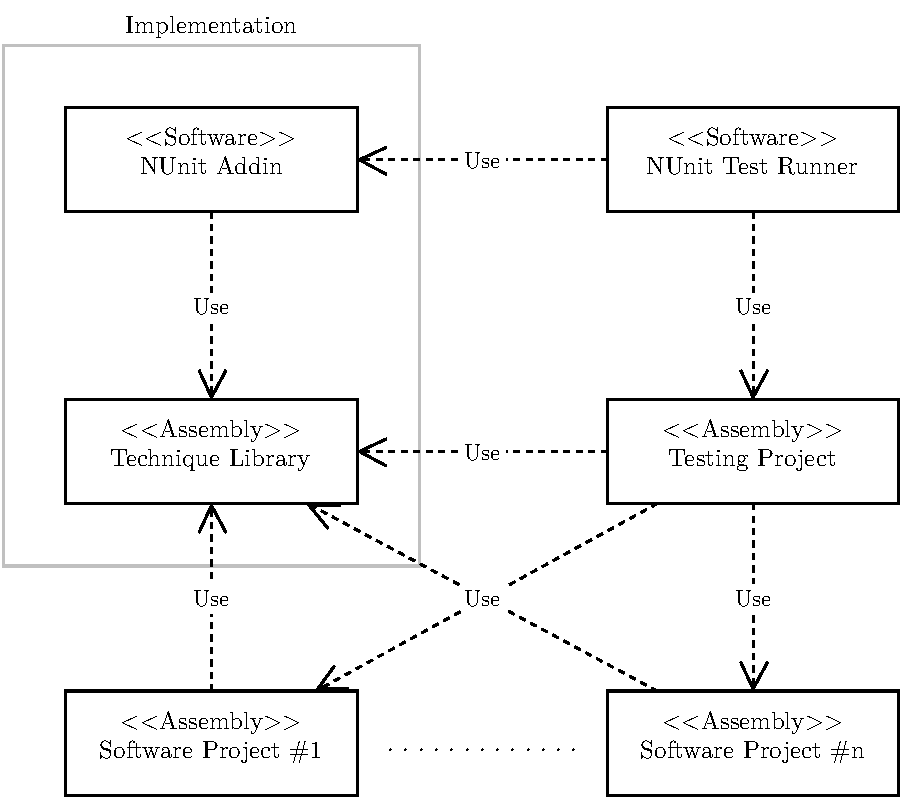
\includegraphics[width=0.9\textwidth]{includes/figures/overview}
  \caption{UML class diagram showing the implementation dependencies.}
  \label{fig:overview}
\end{figure}

When integrating the technique into an existing software development project, the software developer needs to perform several steps in order for the technique to be used. For details on how this integration is performed, refer to section~\vref{sec:technique-integration}.

\subsection{Implementation Details}\label{sec:implementation-details}
In this section, the implementation details of the selected regression testing technique, as presented in section~\ref{sec:technique-description}, are described. The implementation details are separated into the different phases of the technique. Finally, some practical implementation aspects, which have not already been covered for the different phases, are considered.

\subsubsection{Phase 1: Test Case Selection / Affected Class Diagram (\gls{acd})}\label{sec:impl-p1}
The first phase consists of two steps; generation of the \gls{acd} and performing the actual test case selection. However, according to the algorithm description by \citet{mansour2009regression}, some information needs to be given as input to the algorithm. 
Therefore, the following list of steps for the first phase also details the prerequisites for being able to generate the \gls{acd} and perform the test case selection.

\begin{enumerate}[label=P1.\arabic*]
  \item\label{itm:impl-p1:1}\textit{The set of modified and deleted methods and the affected classes}. By determining which methods are affected we also find out which classes have been affected, since we know in which class each method belongs.
  \item\label{itm:impl-p1:2}\textit{The class diagram of the whole program}. This is used for finding base class to subclass relations and finding overridden methods in subclasses. This is also required in order to find all classes in the whole program.
  \item\label{itm:impl-p1:3}\textit{The test case-method coverage information}. This is a mapping of test cases against the methods being executed when the test case is run.
  \item\label{itm:impl-p1:4}\textit{Generate the Affected Class Diagram (\gls{acd})}. The affected class diagram is then generated using the information from \ref{itm:impl-p1:1} through \ref{itm:impl-p1:3}.
  \item\label{itm:impl-p1:5}\textit{Perform the test case selection}. The actual test case selection can then be performed by utilizing the affected class diagram obtained in \ref{itm:impl-p1:4}.
\end{enumerate}

So, in order to be able to implement the \gls{acd} generation and test case selection algorithms, we first need to determine \ref{itm:impl-p1:1} through \ref{itm:impl-p1:3}. The implementation descriptions for these prerequisites are described first, followed by the descriptions for generation and selection.

\paragraph{\ref{itm:impl-p1:1} Finding the set of modified and deleted methods.} Considering the compilation process of a C\# program, there are three different possible states of a program for which an analysis could be performed. These states are \textit{source code}, \textit{\gls{il} code}, and \textit{assembly code}. A program starts out as source code and is then compiled into \gls{cil} code by the C\# compiler. Finally, the 
\gls{jit} compiler (\gls{jitter}) in the \gls{clr} of the \gls{cli} translates the \gls{il} code into native code for the executing system. \citep{rahman2012expert} Since the \gls{il} code is compiled as it is being read, it is not practical to perform an analysis on the assembly code, as the whole program is never fully compiled. The assembly code for the same \gls{il} code will also vary depending on the execution platform, which is an undesirable property when analyzing the system. We would not like to get different results for different platforms unless changes have been introduced. The assembly code is therefore not a very suitable target for analysis.

The source code format of a program is a human-readable format for which static program analysis can be performed. However, by analyzing the source code, we are essentially performing the same work as a compiler is already doing, in order to determine information about the program. For example, we would have to somehow be able to parse the syntax of the programming language and later determine which methods have been affected by looking at changes in source code between two versions. This could prove very difficult; imagine, for example, how one would handle methods moving location in the source code and changed method definitions, like in code~example~\ref{lst:difficult}. In this example, the method definition and method body has changed, and the method has moved location by one line. Even though it is a simple example, it would require some significant parsing and analysis. The problem seems to be that we are trying to perform a difficult analysis which would require us to write parts of a compiler for this purpose. This would require considerable effort; better would be if we could reuse the existing one.

\begingroup
\captionsetup{type=listing}
\begin{multicols}{2}
\noindent
{\footnotesize
\begin{minted}[linenos]{csharp}
public int Sum(int a, int b)
{
  return a + b;
}
\end{minted}
(a) Initial version of the code example.
}

\columnbreak
\noindent
{\footnotesize
\begin{minted}[linenos]{csharp}
/* Sum of all specified integers. */
protected int Sum(params int[] ints)
{
  return ints.Sum();
}
\end{minted}
(b) Modified version of the code example.
}
\end{multicols}
\captionof{listing}{Illustration of the difficulties of analyzing source code.}
\label{lst:difficult}
\endgroup

\ \\\indent The final format to consider is the \gls{il} code. For this format, the C\# compiler has already processed the source code and generated an intermediary format between source code and native assembly code. This means that the compiler has already analyzed the source code and indirectly extracted the information needed to later compile the program to assembly code. This means that if we can read the \gls{il} code, we should be able to access the information we need to find changed methods. Luckily, there are frameworks, such as Mono.Cecil\footnote{For more information, see \url{http://www.mono-project.com/Cecil/}.}, for the very purpose of inspecting \gls{il} code of programs.

So it seems that inspecting \gls{il} code is the reasonable choice here. Since we want to find the modified and deleted methods (\ref{itm:impl-p1:1}), we need a way identify and compare class definitions, method definitions, and method bodies across two versions of the same program. The following list describes the implemented approach for identification and comparison. Comparisons are only done from the previous version to the next, not for the reverse case.

\begin{itemize}
  \item For \textit{class definitions}, the full name definition can be retrieved, which includes, for example, the package of the class and its name. This is how the class is defined according to the \gls{il} format. Classes are then compared by comparing all methods in the previous version with the methods in the next version, as described below.
  \item Considering \textit{method definitions}, they are also identified using their full name definition, which, for example, includes the return type, full name of the containing class, the name of the method, generic types, and the list of parameter types. This is how methods are defined according to the \gls{il} format. Methods are then compared by comparing all instructions in the method body, as described below.
  \item Finally, for \textit{method bodies} there is no need to consider some kind of identification, since we are only concerned with identification down to method level. Instead, instructions need to be compared. Since instructions are essentially lines of strings, we can compare the list of instruction strings between the two versions of the program. This way we can find out if a method has changed or not.
\end{itemize}

Using the described identification approach means that anything affecting the class or method definition will result in the method seen as deleted in the next version, and that another, new method, has been added. This will also be the case, for example, when renaming the class or method. For an evaluation of this approach, refer to section~\vref{sec:implementation-evaluation}.

\paragraph{\ref{itm:impl-p1:2} Obtaining the class diagram of the program.} 
From the class diagram, we need to determine (1) base classes for modified classes and (2) subclasses to modified classes where a modified methods is overridden. For finding base classes, Mono.Cecil supports finding the base type for any given type. This can be performed iteratively in case it is necessary to determine the whole inheritance hierarchy. Since Mono.Cecil can traverse all classes in a program, it is then trivial to determine (1) for the  program. Code~example~\vref{lst:base-classes} provides a simple recursive implementation showing how the inheritance hierarchy can be determined for any given type.

\begin{listing}[htbp]
{\footnotesize
\begin{minted}[linenos]{csharp}
public static string GetBaseTypes(TypeDefinition type)
{
  if (type.BaseType == null || type.BaseType.FullName == null)
    return string.Empty;

  if (type.BaseType.FullName == "System.Object")
    return " -> " + type.BaseType.FullName;

  return " -> " + type.BaseType.FullName + 
    GetBaseTypes(type.BaseType.Resolve());
}
\end{minted}
}
\caption{Using Mono.Cecil to determine the inheritance hierarchy.}
\label{lst:base-classes}
\end{listing}

Also since Mono.Cecil can iterate through all classes for a program, we can determine the subclasses to modified classes, using the approach described above. Overridden methods are marked in C\# using the mandatory \textit{override} keyword. Mono.Cecil supports checking whether a method is an overridden method. Coupling overridden methods with classes for which base types are modified, we can also determine (2) for the program.

\paragraph{\ref{itm:impl-p1:3} Tracing method invocations for test case-method coverage.} The last piece of information to obtain, in order to be able to perform the test case selection, is the test case-coverage information. Basically, we need to know which methods, in which classes, are being executed whenever a test case executes. The three most important criteria to consider for tracing is that (1) we do not want to modify existing code and we do not want to have dependencies to logging classes, (2) there should be little manual work required to enable tracing for an existing project, and (3) tracing information needs to be stored so that it can be programatically accessed when needed.

\citet{mansour2009regression} suggests to use a trace file for logging method invocations, but does not provide implementation details to realize such logging. The trace class within the C\# language provides a way to trace code execution within an application. Tracing works similar to any form of output; provide some text and it is recorded somewhere, for example to a file. See code~example~\vref{lst:trace} for how tracing statements are used.

\begin{listing}[htbp]
{\footnotesize
\begin{minted}[linenos]{csharp}
public static void Main(string[] args) {
  Trace.WriteLine("Called: Main");
}
\end{minted}
}
\caption{Typical usage example of the C\# trace class.}
\label{lst:trace}
\end{listing}

The obvious problem with trace statements is that we do not want to add them to every method in the program, violating criterion (1). Also, it would be tedious to add such trace statements, which violates (2). However, logging at code level is a cross-cutting concern, for which \gls{aop} is suitable. \gls{aop} allows to perform logging and at the same time  avoid code duplication and dependencies in our program. 

For C\#, PostSharp\footnote{See \url{http://www.postsharp.net/} for more information on this framework.} is an \gls{aop} framework that supports tracing. Essentially, what PostSharp allows us to do, is to create a trace attribute which can easily be attached to all methods in a project. An attribute is a way of associating declarative information with a program entity, such as methods, and later query them during runtime. PostSharp contains extensible attributes which are suited for logging method invocations, so that we can execute arbitrary code whenever a method is invoked, for example, log the methods name and the full name of the declaring type. See code~example~\ref{lst:trace-annotation} for an example of such an attribute. Note that some implementation details have been left out for the sake of simplicity.

\begin{listing}[tb]
{\footnotesize
\begin{minted}[linenos]{csharp}
public class TraceMethodInvocationsAttribute : OnMethodBoundaryAspect
{
  public override void OnEntry(MethodExecutionArgs args)
  {
    var method = args.Method;
    var type = method.DeclaringType;

    Trace.WriteLine(string.Format("Called: {0}.{1})", 
      type.FullName, method.Name));
  }
}
\end{minted}
}
\caption{Attribute which can be used to trace method invocations.}
\label{lst:trace-annotation}
\end{listing}

PostSharp then allows us to declare that the annotation should be attached to every method in an assembly (software project), using a single line of code, without modifying any existing classes in the project except for the \textcf{AssemblyInfo} class. The \textcf{AssemblyInfo} class contains general information describing the assembly; it can be seen as metadata information. Code~example~\vref{lst:trace-assembly} shows an example of how to attach the attribute in code~example~\vref{lst:trace-annotation} to all methods of any visibility in an assembly.

\begin{listing}[htbp]
{\footnotesize
\begin{minted}[linenos]{csharp}
[assembly: 
  TraceMethodInvocations(AttributeTargetTypes = "com.company.product.*", 
  AttributeTargetMemberAttributes = MulticastAttributes.AnyVisibility)]
\end{minted}
}
\caption{Attachment of a trace attribute to an assembly.}
\label{lst:trace-assembly}
\end{listing}

This means that we have now effectively solved criterion (1) and (2). For criterion (3) we simply need to store the method invocations in a suitable format and location, so that it can be accessed later on when the selection is to be performed. For simplicity, the implementation uses the \gls{json} format and on-disk storage for this purpose. Also note that it is useful to separate test method invocations from application method invocations. This can be done in PostSharp by utilizing support for custom validation code during compile time. For example, one could add an overridden method to the class in code~example~\vref{lst:trace-annotation} that filters out only methods with the NUnit \textcf{TestAttribute} attached, which is used to denote test cases. An example of such filtering can be seen in code~example~\vref{lst:trace-filter}.

\begin{listing}[htbp]
{\footnotesize
\begin{minted}[linenos]{csharp}
public override bool CompileTimeValidate(MethodBase method)
{
  return method.GetCustomAttributes(typeof(TestAttribute)).Any();
}
\end{minted}
}
\caption{Filtering out attachment methods that are not test cases.}
\label{lst:trace-filter}
\end{listing}

Now, all information required for the algorithm has been obtained and following are the implementation details for the two steps of the first phase.

\paragraph{\ref{itm:impl-p1:4} Generate the Affected Class Diagram (\gls{acd}).}
Once the prerequisites in \ref{itm:impl-p1:1} through \ref{itm:impl-p1:3} have been determined, the actual implementation of the generation of the affected class diagram is rather trivial. The pseudocode for the algorithm is given by \citet[p. 4]{mansour2009regression} and it is fairly detailed for understanding most of the implementation aspects.\footnote{Note that the authors have made an error in the algorithm description; on page 4, the sixth line from the bottom reads $M_3 = M_3 \cup n$, which is wrong since $n \in M$ and at the end we set $M = M \cup M_3$, which would then leave $M$ unaltered since $M_3 \subseteq M$. Instead, the correct version would read $M_3 = M_3 \cup m$, where $m$ is a method using an affected method, thereby requiring an \textit{use edge}.}

Using appropriate data types, the actual implementation code is very similar to the provided pseudocode. For example, consider code~example~\ref{lst:impl-basetypes}, where an example implementation for finding and adding base types is given. The implementation closely matches the pseudocode version.

\begin{listing}[htbp]
{\footnotesize
\begin{minted}[linenos]{csharp}
foreach (var affectedClass in AffectedClasses)
{
  ClassDiagram.GetBaseTypes(affectedClass).ToList().ForEach(baseType =>
  {
    AffectedClasses.Add(baseType);
    Edges.Add(new AffectedEdge(affectedClass, baseType, Edge.Inheritance));
  });
}
\end{minted}
}
\caption{Adding base types to the affected class diagram.}
\label{lst:impl-basetypes}
\end{listing}

\paragraph{\ref{itm:impl-p1:5} Perform the test case selection.}
The pseudocode for the test case selection algorithm is provided as the second algorithm by \citet[p. 5]{mansour2009regression}. Again, since all prerequisites have already been determined, the actual implementation is again rather trivial. Worth noting though is that the algorithm is described as if there is method-test case coverage available, rather than the reversed, that is, test case-method coverage. The difference is in whether methods are mapped against test cases or test cases are mapped against methods. However, by having one of them, it can be converted to the other one through a simple transformation. The code required for this is provided in code~example~\vref{lst:impl-convert}. The alternative is to generate both types of coverage, which results in an adjacency table; this is the approach used by \citet{mansour2009regression}.

\begin{listing}[htbp]
{\footnotesize
\begin{minted}[linenos]{csharp}
var methodToTestCaseCoverage = new Dictionary<..., ISet<...>>();
foreach (var entry in coverageData)
{
  var test = entry.Key;
  var invocations = entry.Value;

  foreach (var i in invocations)
  {
    if(!methodToTestCaseCoverage.ContainsKey(i.Target))
      methodToTestCaseCoverage.Add(i.Target, new HashSet<...>());

    methodToTestCaseCoverage[i.Target].Add(test);
  }
}
\end{minted}
}
\caption{Test case-method coverage to method-test case coverage.}
\label{lst:impl-convert}
\end{listing}

Test case-method coverage information can also be used directly but require a somewhat different algorithm, as presented in code~example~\vref{lst:impl-selection1}. The idea is to, instead of iterating through all methods in the coverage information and finding test cases covering that method, iterate through test cases and see if any invoked methods are modified. The actual implemented algorithm uses this idea but differs somewhat to code~example~\vref{lst:impl-selection1}, as the example is written for the sake of being understandable in the report context. However, this algorithm is equivalent to the one given for method-test case coverage information.

\begin{listing}[htbp]
{\footnotesize
\begin{minted}[linenos]{csharp}
/*
 * For each test case and list of method invocations in the coverage table
 *   If any invoking or invoked method is marked as modified
 *     Add the test case to the set of selected test cases
 */
 var selectedTestCases = ...;
 foreach (var entry in coverageData)
 {
   var test = entry.Key;
   var invocations = entry.Value; 
 
   foreach (var i in invocations)
   {
     if (acd.IsAffectedMethod(i.From) || acd.IsAffectedMethod(i.Target))
     {
       selectedTestCases.Add(test);
       break;
     }
   }
 }
\end{minted}
}
\caption{Selecting test cases using test case-method coverage.}
\label{lst:impl-selection1}
\end{listing}

\subsubsection{Phase 2: Test Case Selection / C\# Interclass Graph (\gls{cig})}
The second phase reduces the number of test cases selected in the first phase. This is done by generating two \gls{cig}s; one for the original program and one for the modified program. A \gls{cig} represents the control flow of the methods in the classes of the \gls{acd}. The control flow is the possible execution paths. The \gls{cig}s are then compared to find differences in control flow, which are differing edges in the \gls{cig} between the two versions. Test cases are then selected based on whether there are differing edges or not.

An implementation of this phase requires being able to analyze the control flow of a program. Determining the control flow of a program, while considering all of the various language constructs of C\#, would in turn require an extensive analysis of the \gls{il} code. However, the \gls{cig} only concerns consecutive statements and method invocations, including calls to external libraries. Also, only the classes in the \gls{acd} are considered for analysis, so the problem size is reduced somewhat compared to analyzing the whole program. Mono.Cecil supports reading the \gls{il} instructions of method bodies and can also help in identifying method calls; see code~example~\vref{lst:impl-selection2} for example code on how this can be done. One would then have to analyze the operand in order to determine which method, in which type and what library, is being called and continue the analysis. It is worth noting that when a program is being executed, the system executing the \gls{il} code is not aware of all of the possible paths in the program; it simply executes the program with the current state, for example, values of variables, in mind. 

\begin{listing}[htbp]
{\footnotesize
\begin{minted}[linenos]{csharp}
foreach (var type in acd.AffectedTypes)
{
  foreach (var method in type.Methods.Where(method => method.HasBody))
  {
    foreach (var instruction in method.Body.Instructions)
    {
      if (instruction.OpCode == OpCodes.Call)
      {
        // Instruction is a method invocation.
        var operand = instruction.Operand;
      }
    }
  }
}
\end{minted}
}
\caption{Identifying instructions that are method invocations.}
\label{lst:impl-selection2}
\end{listing}

So, let us assume that we, in fact, can determine the \gls{cig} for a given \gls{acd}, which seems somewhat reasonable given the previous reasoning. We can then compare the two \gls{cig}s using algorithm 3 described by \citet[p. 7]{mansour2009regression} and find the affected edges where the control flow differs between the two versions. In order to select test cases, we then need to know which test cases execute the affected edges. To determine this, we need to know which edges are being traversed as the test case executes, meaning we need to know which statements or even \gls{il} instructions are being executed. Normally, this can be done by attaching a debugger and manually step through statements, or \gls{il} instructions, as they are being executed. However, test cases are not being executed with a debugger attached, preventing such attachment and potential tracing. This approach is therefore not practical to implement.

An alternative approach would be to modify the \gls{il} code of the assemblies being tested and programatically insert trace statements, or the like, before every branch instruction. This increases the size of the program and likely drastically prolong the execution time due to the rather extensive amount of tracing during runtime. We also have to consider that the insertion of these trace statements would require some signification time. All things considered, it would require considerable efforts to implement such a solution.

The conclusion for the second phase is that it is not practical to implement. This is due to the difficulties of determining edges covered by tests.

\subsubsection{Phase 3: Further Reduction and Prioritization}
The idea of the third phase is to, for each affected method, select a random test case which executes the method. However, when considering reducing the feedback cycle times, we need to know for all test cases whether they are passing or not. This means that we need to ensure an inclusiveness of 100\% for the regression testing technique. If potentially failing test cases are not included, we simply cannot have a \textit{safe} regression technique. The further reduction attempt is therefore not considered for implementation. Would the reduction be implemented, the work would be rather trivial, as it is only a matter of randomly selecting among the available test cases using the test case-method coverage. Here, it would probably have been a good idea to convert test case-method coverage to  method-test case coverage and from that information select a random test case.

For the prioritization technique, we need to determine the number of classes which covers the affected methods covered by a test ($C_{\mathit{NW}}$ in equation~\vref{eq:weighting}). However, as stated previously for the second phase, determining the control flow of test cases is a difficult task which is not practically implementable. Therefore, $C_{\mathit{NW}}$ cannot be determined, as it requires a \gls{cig} of the previous version of the program. In place of $C_{\mathit{NW}}$, the suggested replacement $C_{\mathit{NW}}^{R}$ is the number of classes containing affected methods which are executed for a test case. For example, if a test case executes four methods distributed across three different classes, $C_{\mathit{NW}}^{R}=3$. The new weighting formula, where $C_{\mathit{NW}}^{R}$ has replaced $C_{\mathit{NW}}$, is therefore the following.

\begin{equation}\label{eq:weighting-new}
  W(T_i)= NW \cdot \frac{C_{NW}^{R}}{MT}
\end{equation}

The number of affected methods covered by $T_i$ can be determined from the test case-method coverage information, simply by checking the number of uniquely executed methods. The same thing can be done for $C_{\mathit{NW}}^{R}$ with the difference of considering classes instead of methods. For the total number of methods in the program, $\mathit{MT}$, we can use Mono.Cecil. An example of how to perform this calculation is provided in code~example~\vref{lst:impl-total-methods}.

\begin{listing}[htbp]
{\footnotesize
\begin{minted}[linenos]{csharp}
private static int GetMethodCount(ModuleDefinition module)
{
  return module.Types.Select(type => type.Methods.Count).Sum();
}
\end{minted}
}
\caption{Using Mono.Cecil to calculate the number of methods.}
\label{lst:impl-total-methods}
\end{listing}

Calculating weights according to equation~\vref{eq:weighting-new} is therefore possible. Unfortunately, NUnit does not provide any way to prioritize test cases. Instead, test cases are being run as they are executed. \citep{poole2012test} Extensions of NUnit, denoted \textit{addins}, do not get access to test cases before they are considered for execution, meaning there is no way in NUnit to perform a prioritization of test cases. Therefore, for the sake of implementation, the weights will be calculated but the actual prioritization cannot be performed. Empirical evaluations will still be possible as manual examinations of the test case ordering is required even if the prioritization would have been implemented.

\subsubsection{Practical Implementation Considerations}
The implementation has been written as an addin to the NUnit framework. However, all core functionality has been separated from the addin, so that the addin merely wraps the core and acts as a link between the core and NUnit. It would therefore be possible to write an extension to some other testing framework without conflicting with the NUnit addin. For both the core and the addin, some practical considerations have been made, which are not considered in the three phases of the regression testing technique. These considerations are discussed in the following sections.

\paragraph{Technique Integration}
The NUnit addin allows for seamless integration with NUnit. After performing an initial setup, so that the relevant assemblies can work with the addin, the analysis will be integrated into the normal testing workflow. This means that when the developer chooses to run unit tests, the addin will perform the required analysis and choose to only execute test cases which have been selected. Remaining test cases will be skipped and a reason, such as ''non-fault revealing test cases'', is provided as to why they were not run. Worth noting is that the technique can be used without modifying any existing code in the assemblies, but adding necessary dependencies, such as Mono.Cecil and PostSharp will be required for the projects.

\paragraph{Storage Concerns}
Both test case-method coverage information and previous versions of the involved assemblies needs to be stored in order to later be able to compare differences and apply the regression testing technique. For the implementation, the involved assemblies are simply copied to a known directory, for which the path is configurable by the developer. The test case-method coverage information is also stored in this directory, serialized to some binary format or a human-readable text format using, for example, the \gls{json} format. When considering very large systems, the storage format is more important, as there may be space limitations and performance issues when dealing with too large files. Binary formats should be better performance-wise for such systems, as the formats generally take up less storage space. In-memory storage may be highly relevant for larger systems, completely avoiding slow disk storage.

Between sessions where test cases are executed, the directory storing coverage information and previous versions, needs to be known and the implementation also needs to deserialize the format into objects which the programming language can work with and operate on.

\paragraph{Changing Test Suites}
Typically, for regression testing techniques, it is assumed that the regression test suites are static, meaning they do not change as modifications are introduced to the program. However, in practice, this is not always the case, as test suites may need to change due to changes in the program. We are therefore interested in considering changing test suites.

For new test cases, which should then also be considered regression tests, it is possible to keep a list of known test cases from the previous version. If the test case is unknown, simply execute it and save its coverage information. For deleted test cases, they will simply not be run, but there is a need to delete old coverage information, in order to not cause a conflict if a test case with the same identification would be added to the suite again. As a minor benefit, it also saves physical storage space to remove coverage information that is no longer required.

If test cases are modified, their coverage information may no longer be correct. Here, we need to analyze the project containing the tests to see which tests have been modified and need to be re-executed. This can be performed using the same approach as have already been implemented. Even though test suites contain dependencies resolved by NUnit, such as setup methods which are run before every test case, it does not pose a problem as long as these methods are being traced for coverage information.

\paragraph{Concerned Assemblies}
When developing software, it is possible to split your software into multiple projects or assemblies. These assemblies may be independent modules or they may depend on external components or projects within your solution. It is also common practice to have your tests in a project that is separate to the application. Test case-method coverage information can still be retrieved without any changes, as the developer is responsible for making sure the correct attribute is attached to the project's methods, as described in section~\ref{sec:implementation-details}. However, there is still a need to determine which assemblies should be compared against their previous versions. The implementation deals with this by having the developer specify the paths to the concerned assemblies. These paths can correspond to the output path of the compiler, so that the integration is seamless after an initial configuration.

\paragraph{Considering Failed Tests} 
When using the implemented technique and executing tests, one will eventually find that one or more tests fail, meaning that the program or tests need to be changed. Now, if the developer were to execute the tests again, without making any modifications, the technique would not select any tests for execution, as no differences could be found between the current and previous version. However, in practice, this is not desirable; it would be better if a failing test case is executed again until it runs with a passing status. For this reason, the implementation saves the last result of the test case and automatically includes all test cases which failed the last time, no matter whether modifications were made or not.

\paragraph{Tracing Side Effects}
When PostSharp attaches trace attributes to methods or tests cases, the \gls{il} code of the method changes. There are no guarantees that these changes are equal between two versions of the same program; and as it turns out, they are not. However, as these changes are very local and use PostSharp specific types, they can easily be ignored when comparing method bodies of a method between two versions of a system.

\chapter{Evaluation}\label{chap:evaluation}
This chapter evaluates the implemented regression technique, as described in chapter~\ref{chap:implementation}. First, the implementation is evaluated using an example application, discussing the robustness and limitations of the implementation. Next, the process of integrating the implementation into the project context is described in section~\ref{sec:technique-integration}. Finally, section~\ref{sec:integration-evaluation} evaluates the implemented regression testing technique in the project context.

\section{Implementation Evaluation}\label{sec:implementation-evaluation}
This section aims at evaluating the implementation described in section~\ref{sec:implementation-details}. The following section discusses the robustness of the implementation by evaluating it with a couple of significant cases for an example application. Following, section~\ref{sec:implementation-limitations} considers the limitations of the implementation. Section~\ref{sec:theoretical-improvements} then concludes this section by evaluating the theoretical improvements of using the implemented technique. For an empirical evaluation, refer to section~\vref{sec:integration-evaluation}, where an evaluation on the integration of the technique into the project context is provided.

\subsection{Implementation Robustness}\label{sec:implementation-robustness}
In order to demonstrate that the implementation is robust and working as intended, the technique will be run on an example application for some significant modifications. The example application is an object-oriented design modelling vehicles, as presented in figure~\vref{fig:application}. For evaluation purposes, we do not consider whether the example application has a good design or not, and instead shift focus to the implemented technique. Note that the evaluation is not an exhaustive evaluation covering every construct in the C\# programming language, but an evaluation showing that the implementation is robust for the most important cases, as described in the original presentation of the technique by \citet{mansour2009regression}. The prioritization is not evaluated as it is merely a calculation of a simple weight.

\begin{figure}[htbp]
  \centering
  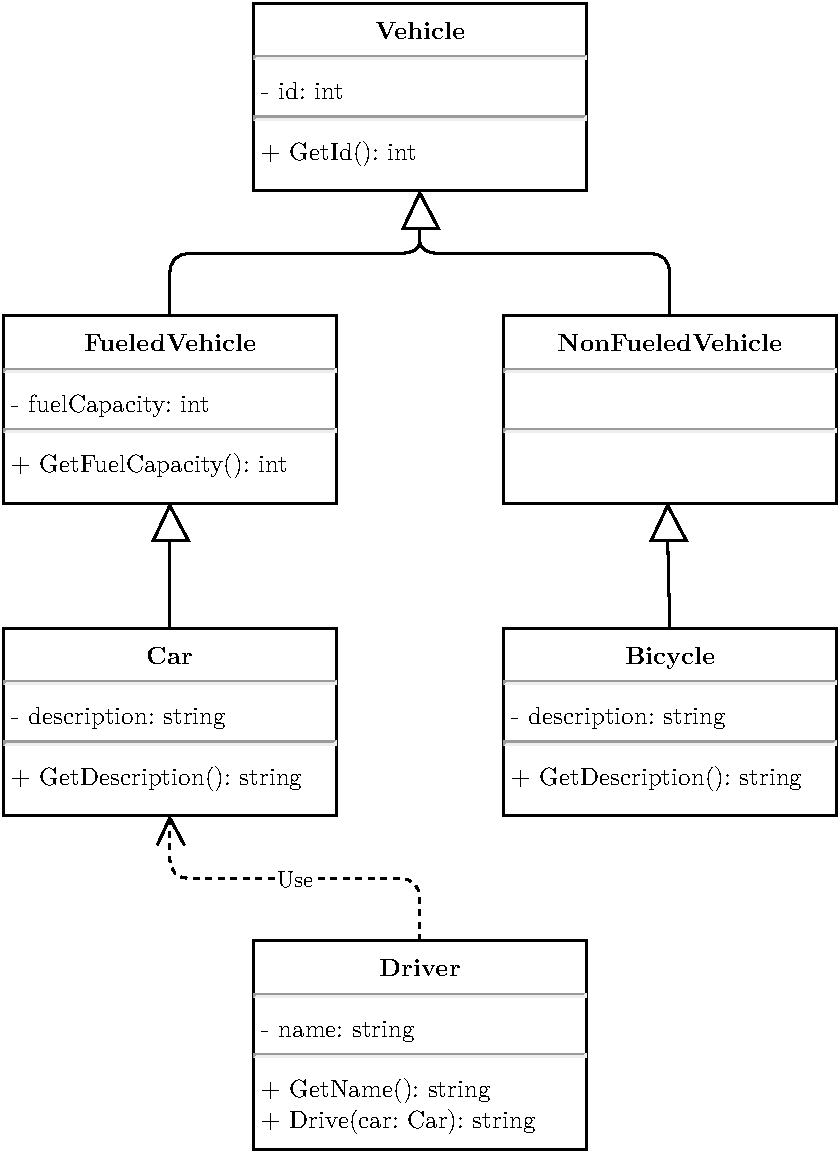
\includegraphics[width=0.9\textwidth]{includes/figures/application}
  \caption{UML class diagram of the example application for evaluation.}
  \label{fig:application}
\end{figure}

The cases of modifications used for evaluation are typical scenarios which the implementation and regression technique should be able to handle. A summary of the evaluation cases are presented in table~\vref{tab:evaluation-summary}. The following sections each consider a single case, in the same order as in table~\ref{tab:evaluation-summary}, and describe how the implementation handles the various modifications. Every evaluation case start with the program presented in figure~\ref{fig:application} and then continue to describe the modifications made to the initial version of the program. Initially, it is assumed that there exists a test suite for every class, and a test case for every method.

\begin{table}[htbp]
  \centering
  \begin{tabular}{|l|l|l|}
    \hline
    \textbf{Case \#} & \textbf{Changed Class} & \textbf{Description}\\
    \hline
    Case 1 & \textcf{Car, Bicycle} & Changing Subclass \& Using Modified Class\\
    \hline
    Case 2 & \textcf{Vehicle} & Altering Base Class \& Indirect Subtypes\\
    \hline
    Case 3 & \textcf{FueledVehicle} & Modification of Constructor Methods\\
    \hline
    Case 4 & \textcf{Driver} & Handling Indirect Method Modifications\\
    \hline
    Case 5 & \textcf{Driver} & Modification of Static Constructors\\
    \hline
  \end{tabular}
  \caption{Summary of the evaluation cases for the implementation.}
  \label{tab:evaluation-summary}
\end{table}

\subsubsection{Case 1. Changing Subclass \& Using Modified Class}
Since testing is performed on methods, changing a class means changing its methods. The three different types of changes that can be made to a class is therefore \textit{add}, \textit{modify}, and \textit{delete}. Renaming a method is a another type of change which can be treated as a delete of the method with the previous name, and an add of the same method but with another name. So, let us consider each type of change; for the \textcf{Car} class, modify the method body of \textcf{GetDescription}. For the \textcf{Bicycle} class, delete the \textcf{GetDescription} method (and related test case) and add a \textcf{GetName} method (and related test case). Table~\vref{tab:evaluation-case1-diffs} shows the differences detected by the technique.

\begin{table}[htbp]
  \centering
  \begin{tabular}{|l|l|l|l|}
    \hline
    \textbf{Change \#} & \textbf{Changed Class} & \textbf{Changed Method} & \textbf{Change Type}\\
    \hline
    Change 1 & \textcf{Bicycle} & \textcf{GetDescription} & Deleted\\
    \hline
    Change 2 & \textcf{Bicycle} & \textcf{GetName} & Added\\
    \hline
    Change 3 & \textcf{Car} & \textcf{GetDescription} & Modified\\
    \hline
  \end{tabular}
  \caption{Detected changes for the first case of implementation evaluation.}
  \label{tab:evaluation-case1-diffs}
\end{table}

From table~\ref{tab:evaluation-case1-diffs}, we can see that the technique has correctly identified the changes made to the program. From these changes, and previously obtained test case-method coverage data, an \gls{acd} can be constructed. The types and edges in the \gls{acd} are presented in table~\vref{tab:evaluation-case1-acd}. The inheritance hierarchy has been identified for the modified \textcf{Bicycle} and \textcf{Car} classes, respectively. Also, since the \textcf{Driver} class is using the \textcf{Car} class, an usage edge is included.

\begin{table}[htbp]
  \centering
  \begin{tabular}{|l|l|}
    \hline
    \textbf{Affected Types:} & \textcf{Bicycle}, \textcf{Car}, \textcf{Vehicle}, \textcf{Driver}\\
                    & \textcf{FueledVehicle}, \textcf{NonFueledVehicle}\\
    \hline
    \textbf{Affected Edges:} & \textcf{Bicycle} $\to$ \textcf{NonFueledVehicle} (Inheritance)\\
                    & \textcf{Bicycle} $\to$ \textcf{Vehicle} (Inheritance)\\
                    & \textcf{Car} $\to$ \textcf{FueledVehicle} (Inheritance)\\
                    & \textcf{Car} $\to$ \textcf{Vehicle} (Inheritance)\\
                    & \textcf{Driver} $\to$ \textcf{Car} (Usage)\\
    \hline
  \end{tabular}
  \caption{Affected types and edges for the first case of evaluation.}
  \label{tab:evaluation-case1-acd}
\end{table}

From the coverage information, we can then use the \gls{acd} to select test cases which cover the changes. The weights, for prioritization of test cases, can also be calculated for the selected test cases. Table~\vref{tab:evaluation-case1-selected} presents the set of test cases and information regarding which tests have been selected, and their weights for prioritization. There are a total of 31 methods in the program. Note that the \textcf{GetDescription} method of class \textcf{Bicycle} is not included as it has been deleted. The added \textcf{GetName} method in \textcf{Bicycle} has been selected because it is a new test case and not previously known. This test case cannot be given any weight as there is no coverage information available until it has been run at least once. The test for \textcf{GetDescription} in the \textcf{Car} class only affects the \textcf{Car} type, while the test for \textcf{Drive} in \textcf{Driver} affects both the \textcf{Driver} and \textcf{Car} types, resulting in a doubled weight.

\begin{table}[htbp]
  \centering
  \begin{tabular}{|l|l|l|l|l|}
    \hline
    \textbf{Class} & \textbf{Test Case} & \textbf{Known} & \textbf{Selected} & \textbf{Weight}\\
    \hline
    \textcf{Bicycle} & \textcf{GetId} & Yes & No &\\
            & \textcf{GetName} & No & Yes & ---\\
    \hline
    \textcf{Car} & \textcf{GetDescription} & Yes & Yes & $1/31$\\
        & \textcf{GetFuelCapacity} & Yes & No &\\
        & \textcf{GetId} & Yes & No &\\
    \hline
    \textcf{Driver} & \textcf{Drive} & Yes & Yes & $2/31$\\
           & \textcf{GetName} & Yes & No &\\
    \hline
    \textcf{FueledVehicle} & \textcf{GetFuelCapacity} & Yes & No &\\
                  & \textcf{GetId} & Yes & No &\\
    \hline
    \textcf{NonFueledVehicle} & \textcf{GetId} & Yes & No &\\
    \hline
    \textcf{Vehicle} & \textcf{GetId} & Yes & No &\\
    \hline
  \end{tabular}
  \caption{Known and selected test cases for the first case of evaluation.}
  \label{tab:evaluation-case1-selected}
\end{table}

\subsubsection{Case 2. Altering Base Class \& Indirect Subtypes}
The first case considered changing a subclass and using a modified class. For this case, let us repeat the process in the first case, except this time for different changes. We begin by overriding the \textcf{GetId} method in the \textcf{Car} class to use a separate numbering for cars. This will be the initial program for this case. We then continue by modifying the body of the \textcf{GetId} method in the \textcf{Vehicle} class. The method \textcf{GetOwner} (and related test case) is also added to \textcf{Vehicle}. Table~\vref{tab:evaluation-case2-diffs} shows detected changes.

\begin{table}[bp]
  \centering
  \begin{tabular}{|l|l|l|l|}
    \hline
    \textbf{Change \#} & \textbf{Changed Class} & \textbf{Changed Method} & \textbf{Change Type}\\
    \hline
    Change 1 & \textcf{Vehicle} & \textcf{GetId} & Modified\\
    \hline
    Change 2 & \textcf{Vehicle} & \textcf{GetOwner} & Added\\
    \hline
  \end{tabular}
  \caption{Detected changes for the second case of evaluation.}
  \label{tab:evaluation-case2-diffs}
\end{table}

As for the first evaluation case, we can then continue to generate the \gls{acd} for the introduced modifications. Table~\vref{tab:evaluation-case2-acd} details the affected types and edges for the \gls{acd} in the second evaluation case. Note the differences from the first case, where a modified subclass caused the base classes to be added to the \gls{acd}. Here, we are only concerned with subclasses where the default behaviour of the base class is overridden, as is the case for \textcf{GetId} in the \textcf{Car} class. Being an indirect subtype means that it can be a subtype in several levels of inheritance, not necessarily a direct subtype, where the class would directly extend the modified base class.

\begin{table}[htbp]
  \centering
  \begin{tabular}{|l|l|}
    \hline
    \textbf{Affected Types:} & \textcf{Car}, \textcf{Vehicle}\\
    \hline
    \textbf{Affected Edges:} & \textcf{Car} $\to$ \textcf{Vehicle} (Indirect Subtype)\\
    \hline
  \end{tabular}
  \caption{Affected types and edges for the second case of evaluation.}
  \label{tab:evaluation-case2-acd}
\end{table}

Finally, table~\vref{tab:evaluation-case2-selected} shows the known and selected test cases with their respective weights. We can see that all tests for \textcf{GetId} in subclasses of \textcf{Vehicle} are recognized and selected for execution, even for classes which are not direct subclasses to \textcf{Vehicle}. Each test case covers one affected method in one class, and there are 32 methods in the program, resulting in a weight of $1/32=0.03125$. The exception is the \textcf{GetId} method in the \textcf{Car} class where a call to the base class is performed in \textcf{GetId}. This means that the test case covers two affected classes, namely \textcf{Car} and \textcf{Vehicle}, and the weight is therefore twice of that of the other test cases. The added test for \textcf{GetOwner} in the \textcf{Vehicle} class is included because it is a new test and we have no coverage information until the test case has been run.

\begin{table}[htbp]
  \centering
  \begin{tabular}{|l|l|l|l|l|}
    \hline
    \textbf{Class} & \textbf{Test Case} & \textbf{Known} & \textbf{Selected} & \textbf{Weight}\\
    \hline
    \textcf{Bicycle} & \textcf{GetId} & Yes & Yes & $1/32$\\
            & \textcf{GetDescription} & Yes & No &\\
    \hline
    \textcf{Car} & \textcf{GetDescription} & Yes & No &\\
        & \textcf{GetFuelCapacity} & Yes & No &\\
        & \textcf{GetId} & Yes & Yes & $2/32$\\
    \hline
    \textcf{Driver} & \textcf{Drive} & Yes & No &\\
           & \textcf{GetName} & Yes & No &\\
    \hline
    \textcf{FueledVehicle} & \textcf{GetFuelCapacity} & Yes & No &\\
                  & \textcf{GetId} & Yes & Yes & $1/32$\\
    \hline
    \textcf{NonFueledVehicle} & \textcf{GetId} & Yes & Yes & $1/32$\\
    \hline
    \textcf{Vehicle} & \textcf{GetId} & Yes & Yes & $1/32$\\
            & \textcf{GetOwner} & No & Yes & ---\\
    \hline
  \end{tabular}
  \caption{Known and selected test cases for the second case of evaluation.}
  \label{tab:evaluation-case2-selected}
\end{table}

\subsubsection{Case 3. Modification of Constructor Methods}
The two previous cases handled various types of changes to methods but did not consider constructor methods. For this case, consider code~example~\vref{lst:evaluation-case3-fueledvehicle} where an example implementation of \textcf{FueledVehicle} is provided. Note that the constructor of the \textcf{Vehicle} class is reused in this example, and the constructor of the \textcf{Car} class also reuses the constructor of \textcf{FueledVehicle}.

\begin{listing}[htbp]
{\footnotesize
\begin{minted}[linenos]{csharp}
public class FueledVehicle : Vehicle
{
  private readonly int _fuelCapacity;

  public FueledVehicle(int id, int fuelCapacity) : base(id)
  {
    _fuelCapacity = fuelCapacity;
  }

  public int GetFuelCapacity()
  {
    return _fuelCapacity;
  }
}
\end{minted}
}
\caption{Example implementation for the third evaluation case.}
\label{lst:evaluation-case3-fueledvehicle}
\end{listing}

Let us consider a change to the constructor of \textcf{FueledVehicle}. The only change detected by the technique is for the constructor \textcf{FueledVehicle(int, int)}. The affected types include \textcf{Vehicle} and \textcf{FueledVehicle} and there is an inheritance edge from \textcf{FueledVehicle} to \textcf{Vehicle}. Finally, let us consider the selected test cases in this case. Table~\vref{tab:evaluation-case3-selected} list the known and selected test cases with their respective weights. As expected, all tests for \textcf{FueledVehicle} has been selected since they use the modified constructor. We can also see that all test cases for the \textcf{Car} class have been selected, since they all use the modified constructor of \textcf{FueledVehicle}. Finally, the \textcf{Drive} method of the \textcf{Driver} class must be included since it uses the \textcf{Car} class.

\begin{table}[htbp]
  \centering
  \begin{tabular}{|l|l|l|l|l|}
    \hline
    \textbf{Class} & \textbf{Test Case} & \textbf{Known} & \textbf{Selected} & \textbf{Weight}\\
    \hline
    \textcf{Bicycle} & \textcf{GetId} & Yes & No &\\
            & \textcf{GetDescription} & Yes & No &\\
    \hline
    \textcf{Car} & \textcf{GetDescription} & Yes & Yes & $2/34$\\
        & \textcf{GetFuelCapacity} & Yes & Yes & $3/34$\\
        & \textcf{GetId} & Yes & Yes & $3/34$\\
    \hline
    \textcf{Driver} & \textcf{Drive} & Yes & Yes & $2/34$\\
           & \textcf{GetName} & Yes & No &\\
    \hline
    \textcf{FueledVehicle} & \textcf{GetFuelCapacity} & Yes & Yes & $3/34$\\
                  & \textcf{GetId} & Yes & Yes & $3/34$\\
    \hline
    \textcf{NonFueledVehicle} & \textcf{GetId} & Yes & No &\\
    \hline
    \textcf{Vehicle} & \textcf{GetId} & Yes & No &\\
    \hline
  \end{tabular}
  \caption{Known and selected test cases for the third case of evaluation.}
  \label{tab:evaluation-case3-selected}
\end{table}

\subsubsection{Case 4. Handling Indirect Method Modifications}
While the previous cases focused on handling direct modifications of methods or constructs in a program's classes, there are ways of indirectly modifying and affecting the execution and return value of methods. For example, one could change field values, or modify getters and setters for properties in a class. For this evaluation case, let us consider what happens when the field that \textcf{GetName} reads from in \textcf{Driver} changes implementation, so that a custom getter and setter is used. Fields in C\# may have custom code for how they are set; such methods are named \textcf{get\_\_}\textcf{field} and \textcf{set\_\_}\textcf{field} for a field with the name \textcf{field}. Note that no changes have been made to any existing methods of the class, and that the field that \textcf{GetName} reads from is not accessible outside of the class, so no explicit tests exist for the field.

Having a look at table~\vref{tab:evaluation-case4-diffs}, which details the detected changes, we can see that the getter and setter for the \textcf{name} property are represented as methods with a special syntax. Both \textcf{GetName} and \textcf{Drive(Car)} uses the new getter and the constructor uses the setter, so these three methods are indeed modified. For the \gls{acd}, the only affected type is the \textcf{Driver} class and there are no affected edges. For the selected test cases, we can see that both test cases for the \textcf{Driver} class are selected, using a weight of $2/34 \approx 0.0588$, as would have been expected. Worth noting for this case is that field values are loaded in the constructors of the class, meaning that changing field values also affects the constructor methods.

\begin{table}[htbp]
  \centering
  \begin{tabular}{|l|l|l|l|}
    \hline
    \textbf{Change \#} & \textbf{Changed Class} & \textbf{Changed Method} & \textbf{Change Type}\\
    \hline
    Change 1 & \textcf{Driver} & \textcf{Driver(string)} & Modified\\
    \hline
    Change 2 & \textcf{Driver} & \textcf{GetName} & Modified\\
    \hline
    Change 3 & \textcf{Driver} & \textcf{Drive(Car)} & Modified\\
    \hline
    Change 4 & \textcf{Driver} & \textcf{get\_\_}\textcf{name} & Added\\
    \hline
    Change 5 & \textcf{Driver} & \textcf{set\_\_}\textcf{name} & Added\\
    \hline
  \end{tabular}
  \caption{Detected changes for the fourth case of evaluation.}
  \label{tab:evaluation-case4-diffs}
\end{table}

\subsubsection{Case 5. Modification of Static Constructors}
Static methods, or class methods, can be treated as regular methods in our regression testing technique, assuming that we are tracing their invocations, so that coverage information can be generated. However, static constructors have to be treated separately. The special thing about them is that they are only executed once, when the class is first used, for example, when another class invokes one of the methods in the class. This means that, when tracing method invocations, the static constructor will only be invoked once, and only one of our tests for the class will show an invocation of the static constructor. However, this is not actually the case, because changes to static constructors could affect every method, static or not, in the class and, in turn, every class using those methods. This is a problem because our coverage information does not include the invocation of the static instructor for every test. For this reason, given a change to the static constructor in a class, the implemented solution marks all methods of the class as modified.

For this case, let us consider a static implementation of the \textcf{Driver} class, where the driver's name is fixed and initialized using a static constructor. Looking at the coverage information, the test for the \textcf{Drive} method has invoked the static constructor, while the test for \textcf{GetName} has not. When changing the name of the driver, the implementation has found that the static constructor has changed. The \textcf{Driver} class is listed as affected, but there are no affected edges. Table~\vref{tab:evaluation-case5-selected} presents the selected test cases and their respective weights. As the test for \textcf{Drive} included a call to the static constructor in the coverage information, it has been selected. The second selected test is the one for \textcf{GetName}, which was selected because it invoked a method in the \textcf{Car} class which had its static constructor modified. The weight for the test for \textcf{Drive} is doubled compared to the one for \textcf{GetName}, which is because the static constructor was included in the coverage information, resulting in two affected methods in the weight calculation.

\begin{table}[htbp]
  \centering
  \begin{tabular}{|l|l|l|l|l|}
    \hline
    \textbf{Class} & \textbf{Test Case} & \textbf{Known} & \textbf{Selected} & \textbf{Weight}\\
    \hline
    \textcf{Bicycle} & \textcf{GetId} & Yes & No &\\
            & \textcf{GetDescription} & Yes & No &\\
    \hline
    \textcf{Car} & \textcf{GetDescription} & Yes & No &\\
        & \textcf{GetFuelCapacity} & Yes & No &\\
        & \textcf{GetId} & Yes & No &\\
    \hline
    \textcf{Driver} & \textcf{Drive} & Yes & Yes & $2/33$\\
           & \textcf{GetName} & Yes & Yes & $1/33$\\
    \hline
    \textcf{FueledVehicle} & \textcf{GetFuelCapacity} & Yes & No &\\
                  & \textcf{GetId} & Yes & No &\\
    \hline
    \textcf{NonFueledVehicle} & \textcf{GetId} & Yes & No &\\
    \hline
    \textcf{Vehicle} & \textcf{GetId} & Yes & No &\\
    \hline
  \end{tabular}
  \caption{Known and selected test cases for the fifth case of evaluation.}
  \label{tab:evaluation-case5-selected}
\end{table}

\subsection{Implementation Limitations}\label{sec:implementation-limitations}
While the previous section focused on the robustness of the implementation, this section discusses the limitations of the implemented technique. The following list briefly discusses some limitations surrounding the technique, while the following sections give some more details around supporting language specific constructs and the choice of test runner for executing tests.

\begin{itemize}
  \item\textit{Limited to use an intermediary format}. The implementation is specific to C\# and analysis of an intermediary format, between source code and assembly code. In this case, the intermediary format is \gls{il} code. While discussing the implementation in section~\ref{sec:implementation-details}, it was seen considerably more difficult to analyze source code and assembly code.
  \item\textit{Does not consider changes in external dependencies}. The technique assumes that all changes, which can affect the status of executing a test case, are code changes. Systems can have external dependencies, which the technique may not be able analyze. If changes in external dependencies affect the status of the test case, the technique may no longer be \textit{safe}, as the technique only detects changes in code.
  \item\textit{Makes no effort to detect renamed methods or classes}. Renaming methods or classes will be seen as deletion of the methods with the previous names and addition of methods with the new names. No effort is made to try and detect methods which have been renamed, which means that all tests executing such methods will be selected for execution.
  \item\textit{Relies on Mono.Cecil for analyzing project assemblies}. The technique completely relies on the Mono.Cecil library for reading information about project assemblies. This means that if the C\# language is updated, Mono.Cecil has to be updated as well to support reading information about programs in the updated language.
  \item\textit{Tracing is limited to the capabilities of PostSharp}. Tracing method invocations for coverage information is limited to the tracing support in PostSharp. As the C\# language is updated, PostSharp will need to support tracing for the updated language for the technique to function.
  \item\textit{Performance is limited due to storage of coverage information}. The technique currently stores coverage information to disk after each run. In the next run, this information is again loaded from disk. An immediate improvement would be to instead keep this information in memory. The evaluations in section~\ref{sec:integration-evaluation} consider both the case when storing it to disk and the theoretical case when it would be kept in memory.
  \item\textit{Does not considering time, space, or performance requirements}. The implementation does not consider any additional requirements, such as a maximum time limit or a maximum amount of disk space or memory space. In some situations, these factors may be limited, and that would require additional considerations of the technique.
  \item\textit{Uses the idea that only code changes affect test execution status}. The technique is based on the assumption that if no code has changed, no tests will run with a different status than the last time they were run. However, this may not always be the case, depending on how the test cases are written. For example, randomized input may be given to methods, resulting in different execution status between runs.
\end{itemize}

\subsubsection{Language Specific Constructs}
\citet{mansour2009regression} describes a technique which mainly focuses on classes and methods within classes. While this is a valid approach, there are several other types of language constructs which are not explicitly considered by the technique, for example, structs and inner classes. The specification of the C\# language \citep{microsoft2013language} covers the many constructs of the language in over 500 pages. While the implementation aims at supporting the majority of these constructs, the magnitude of the language needs to be considered.

Besides the various language constructs in C\#, NUnit also offers a wide range of possibilities for developers when writing test cases. On a theoretical level, one can easily abstract the notion of ''test case'', however, in practice, it is not so easy to determine what makes up a test case. For example, NUnit provides separate setup methods and the ability to run a test case several times with varying input. While these difficulties are not highlighted in the evaluation in section~\ref{sec:implementation-evaluation}, they still need to be considered in practice.

Section~\ref{sec:implementation-robustness} covered the most important evaluation cases for the implemented technique. However, there are still other types and language constructs which have not been covered. \textit{Structs} for example, are handled in the same way as classes. \textit{Delegates} can be used and the invoked methods will be traced like regular methods. Changing \textit{interfaces} may require changes to implementations, and if they do, the changes are treated in the same way as described for the previous cases. \textit{Inner classes} are traced and handled like regular classes. \textit{Attributes} should not affect program execution, assuming there are no external dependencies present which affect the program when using attributes. \textit{Enumerations} are not handled explicitly, but changing the used enumeration constant in a method will cause the method to be modified.

\subsubsection{Test Runner Choice}
A NUnit test runner is a program which finds and executes test cases. Test runners are also responsible for providing addin functionality. NUnit provides its own test runner which can be used together with Visual Studio or separately on its own. A popular extension to Visual Studio is the ReSharper extension, which provides its own test runner. At the time of writing, the ReSharper test runner does not support the same amount of functionality for addins as the test runner part of NUnit. More specifically, the ReSharper test runner does not support event listeners. This is used by the regression technique addin to copy current assemblies and to store coverage information, as described above, after all tests have been executed. The addin will therefore not work with the ReSharper test runner.

\subsection{Theoretical Improvements}\label{sec:theoretical-improvements}
When evaluating the feedback cycle times of the project context in section~\vref{sec:project-cycle-times}, an initial discussion introduced some notation for reasoning about test suites and test cases. Let us use the same notation this time around but instead discuss the improvements when using the implemented regression testing technique. We start by assuming there is a single failing test case and then move on to multiple failing test cases. Following, the differences with integration testing is considered. Finally, a short discussion on the effects of selection and prioritization is given.

Note that the following sections introduce notation for prioritized test cases but the effects of the implemented prioritization are not discussed. This is because it cannot be done on a general level without making assumptions about the test cases. Prioritization is therefore more suited to be evaluated empirically, as is done in section~\vref{sec:integration-evaluation}.

The following discussions do not take into account that there is some initialization time when using a regression testing technique. However, the same reasoning still holds, except that a variable amount of time has to be included for the feedback cycle times when using the technique. The time varies depending on the technique, but for the implementation, the main factor is the size and complexity of the system, as this affects everything from class diagram generation to collecting coverage information.

\subsubsection{Single Failing Test Case}
Let $0 \leq p \leq n$ be the number of selected test cases and let $S = \langle T_{s_1}, \ldots, T_{s_p} \rangle$ denote the set of selected test cases, $S \subseteq T$, ordered by descending prioritization weight, so that $W(T_{s_i}) \geq W(T_{s_{i+1}}),\, \forall\, T_{s_i}, T_{s_{i+1}} \in S$, where $W(T_{s_k})$ is the given weight for test case $T_{s_k}$, $1 \leq k \leq p$. Since the implemented technique is safe, the failing test case has to be in our selection, it follows that, for a failing test case $T_f$, we have that $T_f \in S$ and $f \in \langle s_1, \ldots, s_p \rangle$. This means that the feedback time has been reduced with at least $\sum_{T_i \in (T \setminus S)} E(T_i)$. For the best case, average case, and worst case the following can be said.

\begin{itemize}
  \item For the \textit{best case}, $s_1 = f$ and the feedback time is $E(T_{s_1})=E(T_f)$. This is the same as without a selection technique, but the spread is less with a technique, since there are now fewer test cases being executed. 
  \item When considering the \textit{average case}, without prioritization, we can say that $f=s_{p/2}$ and the total feedback time is $\sum_{i=1}^{p/2} E(T_{s_i})$. The total execution time has improved with $\sum_{T_i \in (T \setminus \langle T_{s_{p/2+1}},\ldots,T_{s_{p}} \rangle)} E(T_i)$.
  \item In the \textit{worst case}, every $T_i \in S$ have to be executed, so the total feedback time is $\sum_{i=1}^{p} E(T_{s_i})$. Minimum saving: $\sum_{T_i \in (T \setminus S)} E(T_i)$.
\end{itemize}

For passing test cases, we still have to execute all the selected test cases, again resulting in the minimum saving of $\sum_{T_i \in (T \setminus S)} E(T_i)$ and the total execution time of $\sum_{i=1}^{p} E(T_{s_i})$.

\subsubsection{Multiple Failing Test Cases}
When there are several failing test cases, we are still interested in knowing that they are failing as soon as possible. We still have that all failing test cases are in the selected set of test cases, $F = \langle T_{f_1}, \ldots, T_{f_m} \rangle \subseteq S$, since our technique is safe. Lets consider the evaluation where we consider the time for the first $1 \leq k \leq m$ failing test cases to execute. Without a regression testing technique, the time for this is $\sum_{i=1}^{f_k} E(T_i)$. We let $F_S$ denote the set of failing test cases with the same ordering as the set of selected prioritized test cases $S$, so that $W(T_{s_i}) \geq W(T_{s_{i+1}})$ $\forall\, T_{s_i}, T_{s_{i+1}} \in F_S$. Again considering the best, average, and worst case, the following can be said.

\begin{itemize}
  \item In the \textit{best case}, all failing test cases are executed first. The feedback time in this case is $\sum_{T_{f_i} \in F_S} E(T_{f_i})$; the same as without selection.
  \item In the \textit{average case}, we ignore the effect of prioritization and assume that tests are uniformly distributed. Feedback time: $\sum_{i=1}^{\ceil{kp/m}} E(T_{s_i})$.
  \item For the \textit{worst case}, all failing test cases are executed last, so we have to execute all selected tests, with a feedback time of $\sum_{i=1}^{p-m+k} E(T_{s_i})$.
\end{itemize}

For feedback on passing test cases, we still need to execute all failing test cases, again with a minimum saving of $\sum_{T_i \in (T \setminus S)} E(T_i)$ and total execution time of $\sum_{i=1}^{p} E(T_{s_i})$.

\subsubsection{Integration Testing Differences}
Continuing the discussion of integration testing in section~\vref{sec:project-cycle-times}, where the tests are split up, so $T=\langle T_1,\ldots,T_c \rangle\cup\langle T_{c+1},\ldots,T_{n} \rangle$, one approach would be to handle these as two separate cases. Test cases are still split up into two parts, and each part is handled as described above. An alternative approach is to perform selection on the whole set of integration test cases, and instead not split up the set. 

Since we cannot make any general assumptions on where failing test cases are placed, it is more suitable to perform an empirical evaluation. For passing test cases, there is still a need to run the whole set of test cases; the question is whether it is preferable to not split up the set, since we now can selectively execute test cases, rather than running all of them. This can, for example, depend on time constraints when the first part is executing. Perhaps it is not reasonable to consider the whole set of test cases, even though selection is performed, since the execution time would be too long. In practice, this limit is likely not fixed, meaning empirical evaluations could be used to reason about which of these approaches are most practical for a given scenario. 

\subsubsection{Effects of Selection and Prioritization}
Using a selection technique filters out test cases which does not need to be executed. 
For passing test cases, the effect is a guaranteed reduction of the feedback cycle time, assuming that $S \subset T$, which means that at least one test case was not selected.
For failing test cases, selecting tests means that the failing ones will be distributed among a smaller set of test cases, resulting in a smaller spread. This in turn results in a reduced feedback time in all cases; worst case, average case, and best case. This requires a safe technique.

For prioritization, passing test cases are not affected. This is because the feedback for passing test cases incorporates executing all passing tests. Failing test cases are however affected, and depending on the prioritization algorithm, the different cases can be improved or worsened in terms of feedback time. Empirical evaluations can be used to measure prioritization effects.

\section{Technique Integration}\label{sec:technique-integration}
This section covers the integration aspects of the implemented regression testing technique, as described in section~\ref{sec:technique-implementation}. More specifically, the following section describes the general approach for integrating the technique into a development project. Section~\ref{sec:specific-integration-cases} then describes additional steps to be taken when considering specific integration cases.

\subsection{General Integration Procedure}
In order to integrate the implementation into an existing software development project, the dependencies, as seen in figure~\vref{fig:overview}, needs to be set up. For every testing project and software project, the technique library needs to be added as a dependency. PostSharp also needs to be added as a dependency, as it is required in order to generate coverage information.

Continuing, the next step is to enable tracing for software assemblies and testing projects. The attributes for tracing are included in the core library, so all that is left to do is to apply them to the projects. We use one attribute for testing projects and a separate attribute for software assemblies. Code~example~\vref{lst:trace-assembly} shows how the attachment can be done for a single project. This attachment then needs to be performed once for every testing project and software project.

Next, the NUnit addin needs to be installed along with its dependencies. While not recommended, the addin can be included in the testing project, by including its source code. However, this is mainly for development purposes, and not general usage. The general approach is instead to copy the compiled addin and its dependencies to the NUnit addin directory, located in the \textcf{/bin/addins} directory of the NUnit installation directory.

Finally, the technique needs to be configured. This can be done using the settings file of the testing project, typically an \textcf{App.config} file. The information which needs to be provided to the technique library is (1) the path to where the technique should store intermediary files, such as coverage information and previous versions of assemblies, and (2) the paths to the assemblies which are to be analyzed for differences. If one wants to consider changing test suites as well, simply include the path to the testing project among these paths.

In most cases, the steps highlighted above will be sufficient in order to integrate the regression technique with an existing development project. Note that no modifications needs to be made to any existing source code, and the developer does not have to perform any tiresome repetitive tasks in order to get started. After the initial setup, there should be no or very limited need for additional configuration. The process is summarized in the following list.

\begin{enumerate}
  \item For every testing project and software assembly:
  \begin{enumerate}
    \item add a dependency on the technique library, so it may be used.
    \item add a dependency on PostSharp, for attaching trace attributes.
  \end{enumerate}
  \item For every assembly in the development project:
  \begin{enumerate}
    \item add attachment code for test case calls (for testing projects).
    \item add attachment code for method calls (for software assemblies).
  \end{enumerate}
  \item Copy the NUnit addin and its dependencies to the addin directory.
  \item For every testing project, add the following configuration details.
  \begin{enumerate}
    \item The paths to the various assemblies which shall be analyzed.
    \item The path to an intermediary storage, for any storage concerns.
  \end{enumerate}
\end{enumerate}

\subsection{Specific Integration Cases}\label{sec:specific-integration-cases}
This section covers two additional integration cases, which both could require additional steps to be performed in order to use the implemented technique. The first case considers assembly redirection, while the other briefly covers differing PostSharp versions. Both cases relate to the usage of PostSharp, and both of them had to be considered for the project context.

\subsubsection{Assembly Version Redirection}
The .NET Framework support a mechanism called assembly version redirection. What this allows us to do, is to redirect, that is, change which version of a dependency should be used. For example, we can state that version $v_1$ of assembly $x$ should be replaced with version $v_2$ instead. This can be performed in various ways, one of which is to include the redirection in the, previously mentioned, \textcf{App.config} configuration file. Code~example~\vref{lst:assembly-redirect} shows how such a redirection can be performed in practice. \citep{microsoft2014redirect}

\begin{listing}[htbp]
{\footnotesize
\begin{minted}[linenos]{xml}
<dependentAssembly>
  <assemblyIdentity name="someAssembly"
    publicKeyToken="32ab4ba45e0a69a1"
    culture="en-us" />
  <bindingRedirect oldVersion="7.0.0.0" newVersion="8.0.0.0" />
</dependentAssembly>
\end{minted}
}
\caption{Assembly version redirection using the \textcf{App.config} file.}
\label{lst:assembly-redirect}
\end{listing} 

When using PostSharp, there is a requirement that all dependencies for the involved projects need to be known and available. This allows us to trace the methods invoked in the dependencies. While the dependencies for a project can be analyzed, assembly version redirects are not found by default by PostSharp. For this to work, we need to tell PostSharp where the redirects are specified, so that they can be considered. If we're using the \textcf{App.config} approach, we simply need to tell PostSharp where this file is located.

\subsubsection{Differing PostSharp Versions}
It is important that every project in the development project is compiled with the same version of PostSharp. Due to implementation differences between versions, issues may occur when, for example, the technique library uses a different version than the one for the rest of the projects. For guaranteed compatibility, it is best to ensure that all projects use the same version.

\section{Integration Evaluation}\label{sec:integration-evaluation}
This section aims at empirically evaluating the reduction of regression testing feedback cycle times in the project context, while using the implemented technique. The following section begins by describing the general approach for evaluating the integration. Section~\ref{sec:evaluation-cases} then presents the different evaluation cases, while section~\ref{sec:selection-evaluation} continues by using these cases for evaluating the test case selection part of the technique. Following, the test case prioritization part is evaluated in section~\ref{sec:prioritization-evaluation}. The reduction of feedback cycle times is then discussed in section~\ref{sec:evaluation-reduced-feedback-cycles} after which the chapter is concluded.

\subsection{Evaluation Procedure}
Given a change to the system, evaluations are performed by measuring the execution times with and without the implemented technique, and then comparing these times. The amount of selected test cases, their results, and their prioritized order, is also concerned in comparisons. These measurements are then used to reason about the reduction in feedback cycle times.

The process is repeated several times for various changes taken from the version control system of the development project. The commits are selected at random from all the commits which followed for the system at the time of integrating the technique. Changes for every commit are also described.

The evaluation is limited to only consider unit tests as the technique does not handle external dependencies present in the project's integration tests. To be able to use the technique for integration testing, we would need to either handle external, non-code changes, or be able to guarantee that external dependencies do not change. If the technique is not aware of changes in external dependencies, test results may be affected even though the technique does not say that is the case. For example, test cases deemed passing, and therefore skipped, may in fact be failing due to external changes.

\subsection{Evaluation Cases}\label{sec:evaluation-cases}
Seven empirical evaluation cases are presented in this section. The first case is an initial run of all tests cases, which is required in order to gather coverage information. This information is assumed to be available for the other cases. The second case is a re-execution of all test cases, following the first case, without making any modifications to the system or test suites. For the third case and for all following cases, we start from an initial version of the system and then apply the changes in the following commit, which is taken from the project's version control system, as described in the methodology in section~\ref{sec:methodology}. Table~\vref{tab:integration-evaluation-cases-changes} presents the details of the changes for these commits. The details are shown as the number of methods and tests that have been added/deleted/modified for the respective cases. The number of modified classes and test classes are also listed for each case.

\begin{table}[htbp]
  \centering
  \begin{tabular}{|l|c|c|c|c|c|c|c|c|}
    \hline
    \textbf{Case \#} & $\boldsymbol{M_A}$ & $\boldsymbol{M_D}$ & $\boldsymbol{M_M}$ & $\boldsymbol{M_C}$ & $\boldsymbol{T_A}$ & $\boldsymbol{T_D}$ & $\boldsymbol{T_M}$ & $\boldsymbol{T_C}$\\
    \hline
    Case 1 & 0 & 0 & 0 & 0 & 0 & 0 & 0 & 0\\
    \hline
    Case 2 & 0 & 0 & 0 & 0 & 0 & 0 & 0 & 0\\
    \hline
    Case 3 & 2 & 1 & 6 & 5 & 0 & 0 & 0 & 0\\
    \hline
    Case 4 & 0 & 0 & 2 & 2 & 0 & 0 & 0 & 0\\
    \hline
    Case 5 & 0 & 0 & 2 & 1 & 0 & 0 & 0 & 0\\
    \hline
    Case 6 & 0 & 0 & 3 & 2 & 4 & 0 & 4 & 1\\
    \hline
    Case 7 & 0 & 1 & 5 & 3 & 2 & 0 & 0 & 1\\
    \hline
  \end{tabular}
  {\\[2ex]\footnotesize$M_A$: methods added, $M_D$: methods deleted, $M_M$: methods modified, $M_C$: modified classes; $T_A$: tests added, $T_D$: tests deleted, $T_M$: tests modified, $T_C$: modified test classes.}
  \caption{Summary of changes for the seven integration evaluation cases.}
  \label{tab:integration-evaluation-cases-changes}
\end{table}

\subsection{Selection Evaluation}\label{sec:selection-evaluation}
In each of the evaluation cases we start by running the test suites using the regression testing technique. Table~\vref{tab:integration-evaluation-cases-results} presents the results of the execution. In the first case, all 3230 test cases are run with a passing status. When these are re-run without making any modifications, we find that all tests are skipped, which is expected as no modifications have been made. For the following cases, we can see a varying amount of failed, passed, and skipped test cases, where the numbers depend on the changes for the respective cases. Note that we manage to skip a lot of test cases which do not have to be executed, about 95\% or more. The first case is expected to take longer time than the other cases, as all tests are executed. For the other cases, the total run time is 01:12\,$\pm$\,7 seconds ($\pm$ 9.7\%).

\begin{table}[htbp]
  \centering
  \begin{tabular}{|l|c|l|l|l|}
    \hline
    \textbf{Case \#} & \textbf{Time} & \textbf{Failed} & \textbf{Passed} & \textbf{Skipped}\\
    \hline
    Case 1 & 01:36 & 0 (0\%) & 3230 (100\%) & 0 (0\%)\\
    \hline
    Case 2 & 01:05 & 0 (0\%) & 0 (0\%) & 3230 (100\%)\\
    \hline
    Case 3 & 01:19 & 18 (0.55\%) & 161 (4.98\%) & 3051 (94.47\%)\\
    \hline
    Case 4 & 01:08 & 3 (0.09\%) & 141 (4.37\%) & 3086 (95.54\%)\\
    \hline
    Case 5 & 01:19 & 0 (0\%) & 61 (1.89\%) & 3169 (98.11\%)\\
    \hline
    Case 6 & 01:11 & 0 (0\%) & 81 (2.51\%) & 3149 (97.49\%)\\
    \hline
    Case 7 & 01:09 & 1 (0.03\%) & 77 (2.38\%) & 3152 (97.59\%)\\
    \hline
  \end{tabular}
    {\\[2ex]\footnotesize Listed are the number of failed, passed, and skipped test cases.\\ The total run times are shown in the format of \textit{minutes:seconds}.}
  \caption{Summarized tests results for the integration evaluation cases.}
  \label{tab:integration-evaluation-cases-results}
\end{table}

Consider table~\vref{tab:integration-evaluation-cases-timings} where the execution time for different parts of the implemented technique is shown for the evaluation cases. We can see that while $\mathit{ET}_1$, $\mathit{ET}_2$, and $\mathit{ET}_3$ are taking up relatively little time (around 7-12 seconds combined), the main concern is loading coverage information from disk ($\mathit{ET}_1$) and storing updated coverage information to disk ($\mathit{ET}_5$). Since the implementation has not focused on performance, storage of coverage information is done by rewriting all coverage information to disk. This is unnecessary, as only coverage for the selected tests need to be updated. This also results in about the same $\mathit{ET}_5$ for all evaluation cases. $\mathit{ET}_6$ is the time for test execution and collection of coverage information.

\begin{table}[htbp]
  \centering
  \begin{tabular}{|c|c|c|c|c|c|c|c|}
    \hline
    \textbf{\#} & \textbf{Total} & $\boldsymbol{\mathit{ET}_1}$ & $\boldsymbol{\mathit{ET}_2}$ & $\boldsymbol{\mathit{ET}_3}$ & $\boldsymbol{\mathit{ET}_4}$ & $\boldsymbol{\mathit{ET}_5}$ & $\boldsymbol{\mathit{ET}_6}$\\
    \hline
    1 & 01:36 & - & - & - & - & 00:15.89 & 01:20.11\\
    \hline
    2 & 01:05 & 00:23.99 & 00:05.47 & 00:01.68 & 00:00.62 & 00:15.27 & 00:17.97\\
    \hline
    3 & 01:19 & 00:24.51 & 00:08.60 & 00:02.10 & 00:00.62 & 00:16.15 & 00:27.02\\
    \hline
    4 & 01:08 & 00:24.15 & 00:05.97 & 00:02.06 & 00:00.61 & 00:15.94 & 00:19.27\\
    \hline
    5 & 01:19 & 00:24.63 & 00:05.39 & 00:01.64 & 00:00.62 & 00:15.27 & 00:31.45\\
    \hline
    6 & 01:11 & 00:24.35 & 00:07.82 & 00:02.74 & 00:00.61 & 00:15.16 & 00:20.32\\
    \hline
    7 & 01:09 & 00:24.12 & 00:07.63 & 00:02.43 & 00:00.07 & 00:16.07 & 00:18.68\\
    \hline
  \end{tabular}
    {\\[2ex]\footnotesize$\mathit{ET}_1$: load coverage information from disk, $\mathit{ET}_2$: determine differences between versions, $\mathit{ET}_3$: generate affected class diagram, $\mathit{ET}_4$: select test cases for execution, $\mathit{ET}_5$: store updated coverage information to disk. $\mathit{ET}_6$: total minus $\sum_{i=1}^{5} \mathit{ET}_i$. The timings are presented in the \textit{minutes:seconds.centiseconds} format.}
  \caption{Summary of execution times for the integration evaluation cases.}
  \label{tab:integration-evaluation-cases-timings}
\end{table}

Consider then table~\vref{tab:integration-evaluation-cases-timings-compared} where the execution times are compared between when using the technique and when it is not used. An initial look on the $R_1$ timings shows that we have an average run time decrease of about 7 seconds or 9\%. However, it is not completely fair that the storing of coverage information is included in the total run time. When storing coverage information, all selected tests have already been executed, so the results have already been obtained and presented to the developer. Storing coverage information is more of a post-processing step, which should only be included if tests were run continuously, that is, if there were several changes to be tested, so we would need to immediately run tests again. In such a case there would be no time to store coverage information to disk between runs, so it would have to be included. In most cases, one should be able to ignore this additional time. The $R_2$ timings exclude the time of storing coverage information, resulting in an average decrease of about 23 seconds or 29\%.

It is also completely possible to never actually store the coverage information to disk. For example, an in-memory database could be used, or the memory could simply be retained using some other approach. It is therefore of interest to show timings when completely excluding the loading and storage of coverage information. The $R_3$ execution times show this exact scenario. We can observe an average reduction in execution time of about 47 seconds or about 60\%. Note that some additional cost of updating coverage information for executed tests will have to be added. However, the time for such tasks is almost insignificant, so the presented figures should not be far from the actual ones. 

It is fair to point out that these results are for an implementation which has not been written with performance in mind, suggesting there probably are quite a lot of performance optimizations that can be made. For example, from table \vref{tab:integration-evaluation-cases-timings}, we can observe that reading coverage information ($\mathit{ET}_1$) takes longer than writing it ($\mathit{ET}_5$). This is due to the implementation using a relatively slow deserialization technique for the coverage information.

In the next section, the prioritization technique is considered.

\begin{table}[htbp]
  \centering
  \begin{tabular}{|c|c|c|c|l|l|l|}
    \hline
    \textbf{\#} & $\boldsymbol{A_1}$ & $\boldsymbol{A_2}$ & $\boldsymbol{A_3}$ & $\boldsymbol{R_1}$ & $\boldsymbol{R_2}$ & $\boldsymbol{R_3}$\\
    \hline
    1 & 01:36 & 01:20 & 01:20 & \plus 00:17 (22\%) & \plus 00:01 (1\%) & \plus 00:01 (1\%)\\
    \hline
    2 & 01:05 & 00:49 & 00:24 & \minus 00:14 (18\%) & \minus 00:30 (38\%) & \minus 00:55 (70\%)\\
    \hline
    3 & 01:19 & 01:03 & 00:38 & \minus 00:00 (0\%) & \minus 00:16 (20\%) & \minus 00:41 (52\%)\\
    \hline
    4 & 01:08 & 00:52 & 00:28 & \minus 00:11 (14\%) & \minus 00:27 (34\%) & \minus 00:51 (64\%)\\
    \hline
    5 & 01:19 & 01:04 & 00:39 & \minus 00:00 (0\%) & \minus 00:15 (19\%) & \minus 00:40 (51\%)\\
    \hline
    6 & 01:11 & 00:56 & 00:32 & \minus 00:08 (10\%) & \minus 00:23 (29\%) & \minus 00:47 (59\%)\\
    \hline
    7 & 01:09 & 00:53 & 00:29 & \minus 00:10 (13\%) & \minus 00:26 (33\%) & \minus 00:50 (63\%)\\
    \hline
  \end{tabular}
      {\\[2ex]\footnotesize$A_1$: total time with technique, $A_2=A_1-ET_5$, $A_3=A_2-ET_1$; $R_1$ to $R_3$: reduced time compared to before for cases $A_1$, $A_2$, and $A_3$, respectively. Timings in \textit{minutes:seconds}. The before reference time, when not using the implemented technique, is 01:19.}
  \caption{Timings compared to without the technique for the seven cases.}
  \label{tab:integration-evaluation-cases-timings-compared}
\end{table}

\subsection{Prioritization Evaluation}\label{sec:prioritization-evaluation}
In this section, we take a look at how the prioritization part of the technique weighted the different test cases. The results of the prioritization are presented in table~\vref{tab:integration-evaluation-cases-prioritization}. We can see that, because of the selection part of the technique, there are a lot fewer test cases to consider for prioritization - around 2 to 5\% of the original amount. Out of the selected test cases, there are even fewer ones that are actually failing when executed. 

\begin{table}[tbp]
  \centering
  \begin{tabular}{|c|l|l|l|}
    \hline
    \textbf{\#} & \textbf{Selected Tests} & \textbf{Failed Tests} & \textbf{Rankings for Failed Tests}\\
    \hline
    1 & 3230 (100\%) & 0 (0\%)& -\\
    \hline
    2 & 0 (0\%) & 0 (0\%)& -\\
    \hline
    3 & 179 (5.54\%) & 18 (10.06\%) & 16, 17, 18, 27, $\ldots$\,, 77, 98 \\
    \hline
    4 & 144 (4.46\%) & 3 (2.08\%) & 90, 93, 112\\
    \hline
    5 & 61 (1.89\%) & 0 (0\%)& -\\
    \hline
    6 & 81 (2.51\%) & 0 (0\%)& -\\
    \hline
    7 & 78 (2.41\%) & 1 (1.28\%)& 23\\
    \hline
  \end{tabular}
  {\\[2ex]\footnotesize Shown are the total number of selected test cases and the percentage of all tests. The number of failed tests is also shown, along with the percentage of the selected total. Rankings are the execution orders for the failed tests among all selected tests.}
  \caption{Prioritization rankings for the integration evaluation cases.}
  \label{tab:integration-evaluation-cases-prioritization}
\end{table}

The ranking for a test case is the order among all selected test cases in which the test case will be executed. The test case with rank 1 will be executed first, the one with rank 2 next, and so on. The rank is obtained by sorting the selected test cases by the weights assigned to them by the prioritization technique. Take the third evaluation case as an example; when the 16th test case is run, it is the first failing test case. The other failing test cases are executed as test case number 17, 18, and so on.

As test cases are executed in no guaranteed order by NUnit, it is not very meaningful to compare the test case execution order between when using the prioritization and when it is not used. Instead it is more interesting to assume that the test case ordering behaves according to some pattern, for example, uniform distribution, and compare that case when using and not using the technique. Such evaluation is performed in the following section, where the effectiveness of the technique in regard to reducing feedback cycle times is the topic of discussion.

\subsection{Feedback Cycle Times}\label{sec:evaluation-reduced-feedback-cycles}
Previously, section \vref{sec:project-cycle-times} presented some notation for reasoning about feedback cycles. Section \vref{sec:theoretical-improvements} then expanded this notation by considering improvements which reduced the feedback cycle times. We can now use this notation along with the empirical evaluations in the previous sections to reason about the improvements. 

While reasoning about feedback cycles earlier in the thesis, the initialization time of the technique was not considered. However, as we are using empirical evaluations, it is of interest to include it in the following discussions. We use $I$ to denote the initialization time of the regression testing technique for a given evaluation case. When calculating $I$, we assume that coverage information has already been loaded, according to previous discussions, and let $I=\mathit{ET}_2+\mathit{ET}_3+\mathit{ET}_4$, as seen in table~\vref{tab:integration-evaluation-cases-timings}.

Note that the following discussions do not consider the case of integration testing, as it has not been the focus of the implementation or evaluation. However, the previously introduced notation and reasoning still holds.

\subsubsection{Single Failing Test Case}
Let us begin by considering a single failing test. We are going to use the seventh evaluation case, as seen in table~\vref{tab:integration-evaluation-cases-prioritization}, as example in this section. Here we have that $T=\langle T_1,\ldots,T_{3230} \rangle$, and a single failing test case $T_f \in T$. We have also selected some test cases for execution, $S = \langle T_{s_1}, \ldots, T_{s_p} \rangle$. Let us again assume a discrete uniform distribution for test case execution when not using the technique. In order to receive feedback on the failing test case, we need to execute all preceding test cases and the failing test case. The following can be said in the best, average, and worst case, with and without using the technique.

In the \textit{best case}, without the technique, $T_f$ is executed first and the resulting feedback time is $E(T_f)$, meaning we only execute the failing test case. When using the technique, we have assigned weights to the test cases, so the feedback time is $\mathit{FT} = I + \sum_{k=s_1}^{f} E(T_k)$, which means that we execute all test cases with higher or equal weight compared to the failing test case: $\forall\,T_i \mid W(T_i) \geq W(T_f),\, T_i \in S$. Note that while the best case is rather unlikely, the feedback cycle time, in this particular case, will actually be longer when using the technique given that $\mathit{FT} > E(T_f)$. Since $\mathit{FT}$ includes $E(T_f)$ and only positive values, this holds except when $I=0$ and $f=s_1$.

In the \textit{average case}, without the technique, $T_f$ is executed in the middle, so that $f=n/2=3230/2=1615$. The resulting feedback time is $\sum_{i=1}^{1615} E(T_i)$. When using the technique, the feedback time is the same as above, that is, $\mathit{FT} = I + \sum_{k=s_1}^{f} E(T_k)\approx 10.13+\sum_{k=s_1}^{f} E(T_k)$ seconds. If we make the reasonable assumption that all test cases have roughly the same average execution time, so that $t=(60+19)/3230\approx 0.024$ seconds without the technique and $t_r=18.68/78\approx 0.24$ with the technique, we have that $\mathit{FT}\approx 10.13+23t_r\approx15.57$ seconds. This can be compared to the time when not using the technique, which would then be $\sum_{i=1}^{1615} E(T_i)=1615t=39.5$ seconds. For this case, the improvement is $1-\mathit{FT}/39.5\approx 60\%$.

In the \textit{worst case}, without the technique, $T_f$ is executed last, meaning we have to execute every test case. The feedback time is $\sum_{i=1}^{n} E(T_i),\,n=3230$. When using the technique, as for the previous cases, $\mathit{FT} = I + \sum_{k=s_1}^{f} E(T_k)$. Using the same reasoning as before, assuming that every test case has roughly the same execution time, we improve by $1-\mathit{FT}/(\sum_{i=1}^{3230} E(T_i))\approx 80\%$.

For passing test cases, we would have to execute all test cases when not using a technique. With the technique, we have managed to select $p=79/3230\approx 2.44\%$ of the tests for execution. Here, we have that $\mathit{FT}=I+\sum_{i=1}^{p} E(T_{s_i})\approx 10.13+79t_r\approx 29$ seconds, compared to $79$ seconds for without the technique. The savings, in this case, are about 50 seconds or about 63\%. As expected, this value is the same as $R_3$ for evaluation case seven in table~\vref{tab:integration-evaluation-cases-timings-compared}.

\subsubsection{Multiple Failing Test Cases}
Let us now consider the case when there are multiple failing test cases in the test suites. We will be using the third evaluation case, as seen in table~\vref{tab:integration-evaluation-cases-prioritization}, throughout this section, which has 18 failing test cases, $F=\langle T_{f_1},\ldots,T_{f_{18}} \rangle$, and 179 selected test cases $S=\langle T_{s_1},\ldots,T_{s_{179}} \rangle$. The indexes of the failing test cases $F\subset S$ are listed in table~\vref{tab:integration-evaluation-cases-prioritization}. We are considering a discrete uniform distribution and the best, average, and worst case for finding the first $1 \leq k \leq m = 18$ failing test cases.

In the \textit{best case}, without the technique, all failing test cases will have to be executed first, resulting in a total feedback time of $\sum_{i=1}^{k} E(T_i)$. As for a single failing test case, the best case will result in a prolonged feedback cycle time when using the technique. We have that $\mathit{FT}(k) = I + \sum_{i=1}^{r(k)} E(T_{s_i}) > \sum_{i=1}^{k} E(T_i)$ in all cases except where $I=0$ and $S=F\cup\langle T_{s_{m+1}},\ldots,T_{s_{p}} \rangle$, meaning that all failing test cases are prioritized to be run first. Here, $r(k)$ is the position of the $k$:th failing test case in $S$. Fortunately, the best case has a very low probability of occurring, as the $m=18$ tests have to be run first among $3230$ tests. We are more interested in analyzing the average case.

In the \textit{average case}, without the technique, the first $k$ test cases should be within the first $\ceil{\frac{kn}{m}}$ executed tests; the feedback time is $\sum_{i=1}^{\ceil{\frac{kn}{m}}} E(T_i)$. The question here is whether $\mathit{FT}(k) = I + \sum_{i=1}^{r(k)} E(T_{s_i}) < \sum_{i=1}^{\ceil{\frac{kn}{m}}} E(T_i)$ where $s_{r(k)}$ is the $k$:th failing test case in its prioritized order. For the third case, we have that $I=11.32$ seconds. If we assume that every test case executes using the same average time, we have $t=(60+19)/3230\approx 0.024$ seconds for without the technique and $t_r=27.02/179\approx 0.15$ seconds with the technique. For determining $r(k)$, we simply examine the rankings presented for the third case in table~\vref{tab:integration-evaluation-cases-prioritization}. Note that only some of the rankings are provided for illustration purposes. Given that the ranking $r(k)$ is known, it then follows that $\mathit{FT}(k) = I + \sum_{i=1}^{r(k)} t_r = I + t_r r(k)\approx 11.32+27.02/179 r(k)$. Figure~\vref{fig:prioritization-evaluation-cases} shows a plot for $\mathit{FT}(k)$ and $\sum_{i=1}^{\ceil{\frac{kn}{m}}} E(T_i)\approx 3230/18\cdot 0.024k$ for $k\in[1, 18]$. From the figure we can see that for $k\geq 4$, the technique is reducing the feedback cycle times. With the technique, the feedback time, as a function of $k$, grows a lot slower than when not using a technique. The figure also shows the improvements of using the technique as $k$ is being varied. Note that $k=0$ is an invalid case and is not of interest; however, the case when only considering passing test cases is described below. Finally, we note that the improvement in feedback cycle time for executing all 18 failing tests is about $51$ seconds or $66\%$.

\begin{figure}[htbp]
  \centering
  \begin{tikzpicture}
	\begin{axis}[
	width=0.8\textwidth,	
	xmin=1,
	xmax=18,
	ymin=0,
	ymax=85,
	axis lines=middle,
    x label style={at={(axis description cs:0.5,-0.1)},anchor=north},
    y label style={at={(axis description cs:-0.1,.5)},rotate=90,anchor=south},
    xlabel=Failing Tests Executed ($k$),
    ylabel=Total Feedback Time (seconds),
    legend style = { at = {(0.97, 1.37)}},
    legend cell align=left]
	    \addplot+[color=darkblue] coordinates {
	      (1, 0.024 * 3230/18 * 1)
	      (2, 0.024 * 3230/18 * 2)
	      (3, 0.024 * 3230/18 * 3)
	      (4, 0.024 * 3230/18 * 4)
	      (5, 0.024 * 3230/18 * 5)
	      (6, 0.024 * 3230/18 * 6)
	      (7, 0.024 * 3230/18 * 7)
	      (8, 0.024 * 3230/18 * 8)
	      (9, 0.024 * 3230/18 * 9)
	      (10, 0.024 * 3230/18 * 10)
	      (11, 0.024 * 3230/18 * 11)
	      (12, 0.024 * 3230/18 * 12)
	      (13, 0.024 * 3230/18 * 13)
	      (14, 0.024 * 3230/18 * 14)
	      (15, 0.024 * 3230/18 * 15)
	      (16, 0.024 * 3230/18 * 16)
	      (17, 0.024 * 3230/18 * 17)
	      (18, 0.024 * 3230/18 * 18)
		};
		\addlegendentry{Reference; $\sum_{i=1}^{\ceil{\frac{kn}{m}}} E(T_i)\approx 3230/18\cdot 0.024k$};
		\addplot+[color=darkred] coordinates {
	      (1, 11.32 + 27.02/179 * 16)
	      (2, 11.32 + 27.02/179 * 17)
	      (3, 11.32 + 27.02/179 * 18)
	      (4, 11.32 + 27.02/179 * 27)
	      (5, 11.32 + 27.02/179 * 34)
	      (6, 11.32 + 27.02/179 * 35)
	      (7, 11.32 + 27.02/179 * 36)
	      (8, 11.32 + 27.02/179 * 49)
	      (9, 11.32 + 27.02/179 * 50)
	      (10, 11.32 + 27.02/179 * 51)
	      (11, 11.32 + 27.02/179 * 55)
	      (12, 11.32 + 27.02/179 * 57)
	      (13, 11.32 + 27.02/179 * 59)
	      (14, 11.32 + 27.02/179 * 62)
	      (15, 11.32 + 27.02/179 * 66)
	      (16, 11.32 + 27.02/179 * 69)
	      (17, 11.32 + 27.02/179 * 77)
	      (18, 11.32 + 27.02/179 * 98)
        };
        \addlegendentry{Technique; $\mathit{FT}(k)\approx 11.32+27.02/179r(k)$}
        \addplot+[color=darkgreen,mark=triangle,mark options={solid}] coordinates {
	      (1, 0.024 * 3230/18 * 1 - 11.32 - 27.02/179 * 16)
	      (2, 0.024 * 3230/18 * 2 - 11.32 - 27.02/179 * 17)
	      (3, 0.024 * 3230/18 * 3 - 11.32 - 27.02/179 * 18)
	      (4, 0.024 * 3230/18 * 4 - 11.32 - 27.02/179 * 27)
	      (5, 0.024 * 3230/18 * 5 - 11.32 - 27.02/179 * 34)
	      (6, 0.024 * 3230/18 * 6 - 11.32 - 27.02/179 * 35)
	      (7, 0.024 * 3230/18 * 7 - 11.32 - 27.02/179 * 36)
	      (8, 0.024 * 3230/18 * 8 - 11.32 - 27.02/179 * 49)
	      (9, 0.024 * 3230/18 * 9 - 11.32 - 27.02/179 * 50)
	      (10, 0.024 * 3230/18 * 10 - 11.32 - 27.02/179 * 51)
	      (11, 0.024 * 3230/18 * 11 - 11.32 - 27.02/179 * 55)
	      (12, 0.024 * 3230/18 * 12 - 11.32 - 27.02/179 * 57)
	      (13, 0.024 * 3230/18 * 13 - 11.32 - 27.02/179 * 59)
	      (14, 0.024 * 3230/18 * 14 - 11.32 - 27.02/179 * 62)
	      (15, 0.024 * 3230/18 * 15 - 11.32 - 27.02/179 * 66)
	      (16, 0.024 * 3230/18 * 16 - 11.32 - 27.02/179 * 69)
	      (17, 0.024 * 3230/18 * 17 - 11.32 - 27.02/179 * 77)
	      (18, 0.024 * 3230/18 * 18 - 11.32 - 27.02/179 * 98)
        };
        \addlegendentry{Difference; $\sum_{i=1}^{\ceil{\frac{kn}{m}}} E(T_i) - \mathit{FT}(k)$}
	\end{axis}
  \end{tikzpicture}
  \caption{Average case feedback times for varying number of failed tests.}
  \label{fig:prioritization-evaluation-cases}
\end{figure}

In the \textit{worst case}, without the technique, all failing tests are executed last, so the total feedback time is $\sum_{i=1}^{n-m+k} E(T_{s_i})$. Note that it is the same case as when considering passing test cases, except that $k=m$, since all tests have to be executed. $\mathit{FT}(k)$ is still the same as before, so the only difference is that the total feedback time is longer when not using the technique. In the worst case, we have an improvement of about 63 seconds or 82\% for finding the first failing test case. Note though that the worst case scenario is as unlikely to happen as the best case scenario.

Figure~\vref{fig:prioritization-evaluation-cases-2} shows the best, average, and worst case together with the case when using the technique. We also show the case when using the technique but only with the selection part, that is, without the prioritization, given by $\mathit{FT}_S(k)=I+\sum_{i=1}^{\ceil{kp/m}} E(T_{s_i})$. For this case we can see that the prioritization does indeed help in improving the feedback cycle time, even though the selection part of the technique helps in reducing it the most.

\begin{figure}[htbp]
  \centering
  \begin{tikzpicture}
	\begin{axis}[
	width=0.8\textwidth,	
	xmin=1,
	xmax=18,
	ymin=0,
	ymax=85,
	axis lines=middle,
    x label style={at={(axis description cs:0.5,-0.1)},anchor=north},
    y label style={at={(axis description cs:-0.1,.5)},rotate=90,anchor=south},
    xlabel=Failing Tests Executed ($k$),
    ylabel=Total Feedback Time (seconds),
    legend style = { at = {(0.95, 1.5)}},
    legend cell align=left]
	\addplot+[color=darkblue] coordinates {
	      (1, 0.024 * 1)
	      (2, 0.024 * 2)
	      (3, 0.024 * 3)
	      (4, 0.024 * 4)
	      (5, 0.024 * 5)
	      (6, 0.024 * 6)
	      (7, 0.024 * 7)
	      (8, 0.024 * 8)
	      (9, 0.024 * 9)
	      (10, 0.024 * 10)
	      (11, 0.024 * 11)
	      (12, 0.024 * 12)
	      (13, 0.024 * 13)
	      (14, 0.024 * 14)
	      (15, 0.024 * 15)
	      (16, 0.024 * 16)
	      (17, 0.024 * 17)
	      (18, 0.024 * 18)
		};
		\addlegendentry{Best Case; $\sum_{i=1}^{k} E(T_i)$};
		\addplot+[color=darkred] coordinates {
	      (1, 0.024 * 3230/18 * 1)
	      (2, 0.024 * 3230/18 * 2)
	      (3, 0.024 * 3230/18 * 3)
	      (4, 0.024 * 3230/18 * 4)
	      (5, 0.024 * 3230/18 * 5)
	      (6, 0.024 * 3230/18 * 6)
	      (7, 0.024 * 3230/18 * 7)
	      (8, 0.024 * 3230/18 * 8)
	      (9, 0.024 * 3230/18 * 9)
	      (10, 0.024 * 3230/18 * 10)
	      (11, 0.024 * 3230/18 * 11)
	      (12, 0.024 * 3230/18 * 12)
	      (13, 0.024 * 3230/18 * 13)
	      (14, 0.024 * 3230/18 * 14)
	      (15, 0.024 * 3230/18 * 15)
	      (16, 0.024 * 3230/18 * 16)
	      (17, 0.024 * 3230/18 * 17)
	      (18, 0.024 * 3230/18 * 18)
        };
        \addlegendentry{Average Case; $\sum_{i=1}^{\ceil{\frac{kn}{m}}} E(T_i)$}
        \addplot+[color=darkgreen,mark=triangle,mark options={solid}] coordinates {
	      (1, 0.024 * 3230 - 17)
	      (2, 0.024 * 3230 - 16)
	      (3, 0.024 * 3230 - 15)
	      (4, 0.024 * 3230 - 14)
	      (5, 0.024 * 3230 - 13)
	      (6, 0.024 * 3230 - 12)
	      (7, 0.024 * 3230 - 11)
	      (8, 0.024 * 3230 - 10)
	      (9, 0.024 * 3230 - 9)
	      (10, 0.024 * 3230 - 8)
	      (11, 0.024 * 3230 - 7)
	      (12, 0.024 * 3230 - 6)
	      (13, 0.024 * 3230 - 5)
	      (14, 0.024 * 3230 - 4)
	      (15, 0.024 * 3230 - 3)
	      (16, 0.024 * 3230 - 2)
	      (17, 0.024 * 3230 - 1)
	      (18, 0.024 * 3230 - 0)
        };
        \addlegendentry{Worst Case; $\sum_{i=1}^{n-m+k} E(T_i)$}
        \addplot+[color=darkbrown] coordinates {
	      (1, 11.32 + 27.02/179 * 16)
	      (2, 11.32 + 27.02/179 * 17)
	      (3, 11.32 + 27.02/179 * 18)
	      (4, 11.32 + 27.02/179 * 27)
	      (5, 11.32 + 27.02/179 * 34)
	      (6, 11.32 + 27.02/179 * 35)
	      (7, 11.32 + 27.02/179 * 36)
	      (8, 11.32 + 27.02/179 * 49)
	      (9, 11.32 + 27.02/179 * 50)
	      (10, 11.32 + 27.02/179 * 51)
	      (11, 11.32 + 27.02/179 * 55)
	      (12, 11.32 + 27.02/179 * 57)
	      (13, 11.32 + 27.02/179 * 59)
	      (14, 11.32 + 27.02/179 * 62)
	      (15, 11.32 + 27.02/179 * 66)
	      (16, 11.32 + 27.02/179 * 69)
	      (17, 11.32 + 27.02/179 * 77)
	      (18, 11.32 + 27.02/179 * 98)
        };
        \addlegendentry{With Technique (Prioritization); $\mathit{FT}(k)$}
        \addplot+[color=darkorange,mark=diamond,mark options={solid}] coordinates {
	      (1, 11.32 + 27.02/18 * 1)
	      (2, 11.32 + 27.02/18 * 2)
	      (3, 11.32 + 27.02/18 * 3)
	      (4, 11.32 + 27.02/18 * 4)
	      (5, 11.32 + 27.02/18 * 5)
	      (6, 11.32 + 27.02/18 * 6)
	      (7, 11.32 + 27.02/18 * 7)
	      (8, 11.32 + 27.02/18 * 8)
	      (9, 11.32 + 27.02/18 * 9)
	      (10, 11.32 + 27.02/18 * 10)
	      (11, 11.32 + 27.02/18 * 11)
	      (12, 11.32 + 27.02/18 * 12)
	      (13, 11.32 + 27.02/18 * 13)
	      (14, 11.32 + 27.02/18 * 14)
	      (15, 11.32 + 27.02/18 * 15)
	      (16, 11.32 + 27.02/18 * 16)
	      (17, 11.32 + 27.02/18 * 17)
	      (18, 11.32 + 27.02/18 * 18)
        };
        \addlegendentry{With Technique (Selection Only); $\mathit{FT}_S(k)$}
	\end{axis}
  \end{tikzpicture}
  \caption{Best, average, and worst case feedback times for failing tests.}
  \label{fig:prioritization-evaluation-cases-2}
\end{figure}

\chapter{Discussion}\label{chap:discussion}
This chapter discusses the results of the thesis and start by considering constraints limiting the generality of the implemented technique. Section~\ref{sec:technique-efficiency} then discusses the effectiveness and evaluations of the technique, while section~\ref{sec:alternative-approaches} concludes the chapter by briefly discussing alternative approaches for reducing feedback cycle times which have not been considered in the thesis.

\section{Generality Constraints}
One of the main concerns for the implemented technique is generality. According to the definition by \citet{rothermel1996analyzing}, as seen in section~\vref{sec:test-cases-selection-metrics}, generality concerns the extent to which the technique can handle complex modifications, diverse language constructs, and various testing frameworks. This relates to reusability in different contexts.

The most obvious limitation is that the implementation is only applicable to applications and modifications in the C\# programming language. As the implementation of programming languages can vary greatly, it seems reasonable to have separate handling for every language. However, while reasoning about which program format to analyze in section~\ref{sec:implementation-details}, it seemed that the \gls{il} code format was the most suitable option compared to analyzing source code or assembly code. It seemed to be quite difficult to perform a differential analysis on these other formats, perhaps so difficult that it is questionable whether the technique can be applied in situations where an intermediary format is not available. In essence, we have to easily and programatically be able to perform a static analysis of the program. In the case of C\#, the Mono.Cecil framework helped us with this.

Another limitation of the technique is that we do not consider modifications to external dependencies, such as configuration files, databases, or the like. For testing level abstractions above unit testing, such as integration testing and system testing, the whole system and all external dependencies are involved. It is therefore considerably more difficult to use the technique for these types of tests. If considering changes in external dependencies, there is a need for a complementary technique dealing with those changes. \citet{nanda2011regression} presents a technique which handles the case of changes in non-code dependencies, which could be used as reference in case of an implementation considering changes in external dependencies. However, higher testing abstraction levels could still utilize the technique, under the assumption that no changes in non-code dependencies are made during or between test case executions. As a matter of fact, the integration evaluation in section~\ref{sec:integration-evaluation} focused on unit testing exclusively because it was considered very difficult to track changes in external dependencies for integration tests. Integration testing could have been evaluated given that this was not the case.

While the technique was written for NUnit, it does separate the NUnit addin from a core library, as seen in figure~\vref{fig:overview}. This means that other testing frameworks than NUnit in theory could be supported in the future - not limiting the technique to a specific testing framework. However, one of the major problems is being to reliably verify that the technique works as intended. Given the many language constructs in both C\# and NUnit, this is an extensive task. While section~\ref{sec:implementation-evaluation} evaluates the most important language constructs, a complete evaluation would require considerably more effort with increased difficulty. An underlying assumption of test cases are that they, given that no change is made to the program, always execute with the same status. This effectively prevents test cases with randomized parameters, unless we can guarantee that such tests alway run with the same status, even though the parameter values can change with every execution. NUnit supports attributes for randomizing input, which could be considered by the technique. Test cases implementing their own input randomization is more difficult to support.

Interestingly enough is that the implementation can partially be reused in order to handle changing test suites; something that is normally not considered by regression testing techniques. However, in environments where an application changes frequently and in large magnitudes, test cases can change often and quickly. Handling changing test suites can therefore be important, which is considered by partially reusing the technique for test suites.

The implementation should be seen as reusable for other C\# projects, especially since the amount of configuration is limited, and no changes are performed to existing code, while only introducing an extra dependency. However, it is important to recognize that the technique will have to be maintained for future updates to C\#, NUnit, Mono.Cecil, and PostSharp.

\section{Technique Efficiency}\label{sec:technique-efficiency}
\citet{rothermel1996analyzing} defined the efficiency metric, which uses time and space measurements for technique execution and test case execution. One of the major constraints of the technique relates to the size of the coverage information. For programs with many test cases and deep call stacks, the size of the coverage information will be larger than for systems with few tests and shallow call stacks. The implementation has not focused on efficiency in these terms, but it could be a problem for larger programs than the one in the project context. Avoiding to store coverage information to disk between runs, and only keep it in memory, seems to be a good way to both reduce the technique's execution time and disk storage requirements. The problem is to implement such an in-memory approach in practice.

While prioritization was seen to have a noticeable effect when evaluating the technique (see for example figure~\vref{fig:prioritization-evaluation-cases-2}), the prioritization could not be implemented in NUnit. The technique did also not specifically state what weight to assign to new test cases, for which no coverage is available. Also, the second phase of the technique was stated to not be practical to implement, potentially limiting the effectiveness of the technique. However, this loss in effectiveness cannot be measured, and it is also unknown whether such an analysis can be done within reasonable time, so as to not prolong the total test execution time. It can also be argued that it is not necessary to generate the whole \gls{acd} unless the second phase is to be run. There does seem to be more information in the \gls{acd} than what is required for the first phase. Base classes to modified classes, for example, should not be affected if only their subclasses are modified; yet, they are included in the \gls{acd}.

Method identification is one part of the technique which affects the efficiency of the technique. Since no attempts are made to find renamed methods, they will be treated as new methods and new test cases, suggesting that renaming classes or tests affects performance. Perhaps it would be a good idea to try and find renamed parts of the system in order to avoid extra execution time. The problem is how to do this in an efficient and systematic way, so as to not actually increase the total execution time. 

An interesting case arises when the same program is compiled with different compilers or different versions of the same compiler. This could result in changes to many parts of the program, and thereby executing many tests without actually having the need. However, one could argue that, since the program has actually changed, we should therefore also run tests which execute those changes. Essentially, we are verifying whether the compiler compiled the program without introducing any faults.

Given that we can deal with coverage information, we have seen that the implemented technique in fact can be usable and that it reduces the feedback cycle times. The selection part allows us to reduce the total number of test cases to be executed; improving the feedback cycle times for both failing and passing test cases. The prioritization then further helps in allowing us to potentially execute failing test cases earlier on in the execution process. It is not evident in which scenarios it is suitable to use the technique and in which cases it is not suitable. We are essentially trading test execution time against time for analysis, roughly meaning that if the analysis time is greater than the time for executing the skipped test cases, the technique should not be used. In practice, some basic experiments, similar to the ones seen in this report, could be conducted to find out if the technique is suitable.

One of the main drawbacks when evaluating the technique is that we are comparing with the case when tests are uniformly distributed. In practice, this may not actually be the case. Even though NUnit gives no guarantees on the order of test case execution, in reality, it executes test cases in the same test suite in sequence. In cases when, for example, one writes one test suite per class, changing that class will more likely affect the associated test suite than other parts of the program. There may as well be other test suites for other classes which uses the modified class, resulting in some spread of failing test cases. The actual execution order varies from project to project, suggesting that it is not very reasonable to compare with the actual order.

\section{Alternative Approaches}\label{sec:alternative-approaches}
There are alternative approaches for reducing feedback cycle times, which the thesis has not considered --- for example, minimization techniques. The problem with minimization techniques is that it is difficult to reliably remove redundant test cases from test suites. The problem lies in the definition of redundant, where a very desirable definition is that: a test case $T_1$ is redundant if and only if there exists another test case, $T_2$, such that the status of $T_1$ is always equal to that of $T_2$ when both tests are executed. However, proving that definition of redundant is very difficult and research instead use various coverage criteria for defining redundant. Tests may also have been written to document behavior of classes, so removing them completely could actually be like removing part of the documentation for a system - something that is most likely undesirable.

Parallelization is an approach not considered in the thesis. Parallelization could prove to be an effective way of decreasing feedback cycle times, both parallelization of test cases and test suites. The next version of NUnit has planned support for running multiple test cases in parallel \citep{poole2013parallel}.

\section{Possible Future Work}
Following are some suggestions for possible future work.

\begin{itemize}
  \item\textit{Improve performance of the implementation}. An immediate improvement would be to keep coverage information in memory instead of loading and storing it to disk. As the focus has not been on performance, there are likely a lot more optimizations which can be done.
  \item\textit{Extend functionality of the NUnit test runner}. Due to limitations of the test runner, it was not possible to integrate the prioritization with the NUnit framework. Future work could possibly extend NUnit's existing functionality, so as to enable test case prioritization.
  \item\textit{Continue to extend and evaluate supported constructs}. As there are an extensive amount of C\# language constructs and NUnit constructs, further work could evaluate and add support for even more constructs.
  \item\textit{Investigate the possibilities of multi-objective approaches}. It would be interesting to see if multi-objective techniques would be possible and yield reduced feedback cycle times. Such techniques would consider several additional constraints; time, space, performance, and more.
\end{itemize}

\chapter{Conclusions}\label{chap:conclusions}
In this thesis we have seen an implementation of a regression testing technique which used both test case selection and test case prioritization strategies. The implementation relied on having an intermediary format on which static analysis could be performed. The selection technique has been integrated with the NUnit framework through an addin and evaluated both theoretically and empirically, admitting it is difficult to verify that all language constructs and NUnit constructs are supported. The implementation has then been extended by also considering changing test suites using the same technique.

Using empirical evaluations, the technique has been shown to be able to reduce regression testing feedback cycle times. For both feedback on passing and failing test cases, where the failing tests cases were assumed to be uniformly distributed, improvements of about 50 seconds or 66\% were observed when using the technique. The selection technique was determined to be efficient, often selecting at most a few percent of all test cases for execution. The prioritization technique was seen to help reduce the feedback time for failing test cases when they were assumed to be uniformly distributed. The implementation has not specifically focused on performance; the next logical step would be to try to keep coverage information in memory.

It is important to evaluate whether the technique is suitable on a per-project basis, so as to verify that it actually improves feedback cycle times for a certain project.  Such evaluations could be similar to the ones presented in this thesis. Alternative approaches could be to use a test suite minimization strategy or consider parallel execution of test cases.

% References
\cleardoublepage\phantomsection
\addcontentsline{toc}{chapter}{References}
\bibliographystyle{plainnat}
\bibliography{includes/references}

% Appendices
\begin{appendices}
  \chapter{Interview Plan}\label{app:interview-plan}
The interview plan is based on \citet{jacobsen1993intervju, annika1993intervju}.

\textit{Interviewer} is \author, student in Information Technology (IT) at Linköping University, performing a master's thesis in relation to regression testing. \textit{Respondent} is a software developer working in the project context for the thesis work. The interviewer and respondent are employees of the same company but have never been working together on the same project. Preceding the interview, a meeting between the interviewer and respondent has been held, where the current test setup was explained and the perceived problems discussed.
 
The main \textit{purpose} of this interview is to determine if there are any perceived problems with the current test setup and if so, which type of testing is deemed problematic. The other purpose is to allow for questions regarding the current test setup, improvement work, and knowledge of regression testing techniques. The interview is \textit{semi-structured}, which means that the interview questions are used as a guideline, rather than not allowing any diversion from the questions.
  
The \textit{location} of the interview will be a meeting room of the company, familiar to the respondent, at 14:00 on a Monday, for the duration of an hour. The meeting room has a neutral and sparsely decorated environment, with eight chairs and a round table. Windows have been covered so as to ensure that no visible events occurring outside may be of a distracting nature. 

The \textit{background information} for the interview is the information provided in the background of the thesis, as described in section~\ref{chap:background}. From this information, and in relation to the problem description, a set of questions have been identified. These questions are listed in the following section, grouped by their respective question areas and in the order they will be asked during the interview, along with follow-up questions.

The interview will be \textit{recorded} in its entirety for the sake of later being able to include the transcription in the report. While the interview is progressing, notes will be taken, which will help in asking relevant follow-up questions. The recording will be transcribed and the respondent will be asked if the transcription is correct or not before it is included in the report. Statements regarded as incorrect will either be changed according to the respondents clarifications or excluded from the report. The communication after the interview will be handled using internal company email correspondence. If there is a need to ask follow-up or clarifying questions after the interview (for example, if certain parts of the recording is of low audio quality), this will be handled in the same manner. Any changes or additions after the interview will be clearly marked in the transcription. See appendix~\vref{app:interview-transcription} for the transcription of the interview.

Regarding potential \textit{ethical issues}, the respondent's identity will be kept anonymous. In case any sensitive details may be part of the interview, the respondent will be asked whether any details need to be censored. This will be part of the respondent's review of the transcribed interview dialogue. Apart from reviewing the transcription, the respondent will have no possibility to affect the final results. The respondent will not be able to review the interview questions before the actual interview and no payment will be given for taking part in the interview. After the thesis work has been completed, the respondent will be able to read the final report for which the interview was performed. A company-wide presentation of the thesis work will also be held, at which the respondent is free to participate.

The \textit{expected result} of the interview is to be able to further specify the perceived problems with regression testing in the project and, in turn, help with formulating the problem description of the thesis. The secondary result is to gain a better understanding of the current test setup, improvement work on the test suites, and knowledge of regression testing techniques.

\tocless\section{Interview Questions}\label{app:interview-questions}
In the following section, the original interview questions are given in Swedish. These are the questions which were asked during the interview. For readers who cannot understand Swedish, the questions have been freely translated to English in the section following the original questions.

\vspace{1ex}
\tocless\subsection{Original Questions (Swedish)}
The following questions are the original questions asked during the interview. They are available in their original form as follows and available freely translated to English in the following section.
x
\vspace{1ex}
\begin{otherlanguage}{swedish}
\begin{enumerate}
  \item\label{itm:int:role} Skulle du i grova drag kunna förklara din roll i projektet?
  \begin{enumerate}
    \item\label{itm:int:role:a} Hur kommer arbetet med testningen in i detta arbete?
    \item\label{itm:int:role:b} Skulle du kunna förklara hur detta praktiskt fungerat?
    \item\label{itm:int:role:c} Hur många är ni som arbetar med vidareutveckling av testerna?
    \item\label{itm:int:role:d} Arbetar ni efter någon speciell utvecklingsmetod eller tankesätt?
    \begin{enumerate}
      \item\label{itm:int:role:d:i} Har testerna tagits fram enligt denna metod eller tankesätt?
      \item\label{itm:int:role:d:ii} Hur tycker du att det har fungerat att arbeta på det sättet?
    \end{enumerate}
    \item[$(*)$] Summera och fråga om utvecklingsmetoder rörande testningen.
  \end{enumerate}
  
  \item\label{itm:int:setup} Skulle du kunna förklara hur nuvarande test setup ser ut?
  \begin{enumerate}
    \item\label{itm:int:setup:a} Ser du några problem med hur er test setup ser ut?
    \item\label{itm:int:setup:b} Varför upplevs detta som problem med er test setup?
    \item\label{itm:int:setup:c} Vilka olika typer av tester använder ni i projektet?
    \item\label{itm:int:setup:d} Brukar er setup förändras något eller är den fastställd?
    \item[$(*)$] Summera och fråga om nuvarande test setup i projektet.
  \end{enumerate}
  
  \item\label{itm:int:test} Kan du beskriva hur en utvecklare bör testa sina ändringar i projektet?
  \begin{enumerate}
    \item\label{itm:int:test:a} Vad tror du skulle kunna förbättras i arbetsprocessen?
    \item\label{itm:int:test:b} Upplever du att testningen tar för lång tid?
    \item\label{itm:int:test:c} Vilka typer av tester är det som tar för lång tid?
    \item\label{itm:int:test:d} Varför är det problem att det tar för lång tid?
    \item\label{itm:int:test:e} Upplever utvecklarna att tiden för testerna är problematisk?
    \item[$(*)$] Summera och fråga om problemen rörande testningen.
  \end{enumerate}
  
  \item\label{itm:int:improve} Kan du förklara hur ni arbetat med att förbättra era test suites?
  \begin{enumerate}
    \item\label{itm:int:improve:a} Har du några tankar eller idéer på förbättringar som skulle kunna göras för att förbättra era test suites?
    \item\label{itm:int:improve:b} Känner du till några verktyg eller metoder som skulle kunnas användas för att förbättra testningen?
    \item\label{itm:int:improve:c} Har ni arbetat något med att använda urval av testfall för att det tar för lång tid att köra alla tester?
    \begin{enumerate}
      \item\label{itm:int:improve:c:i} I vilka fall har urval av testfall gjorts?
      \item\label{itm:int:improve:c:ii} Hur har dessa urval av testfall genomförts?
      \item\label{itm:int:improve:c:iii} Hur tror du att urval av testfall kan förbättra testningen?
    \end{enumerate}
    \item\label{itm:int:improve:d} Har ni arbetat något med att rangordna eller prioritera testfall?
    \begin{enumerate}
      \item\label{itm:int:improve:d:i} Görs det någon prioritering av testfall i dagsläget?
      \item\label{itm:int:improve:d:ii} Vad skulle vara vettigt att basera en sådan prioritering på?
      \item\label{itm:int:improve:d:iii} Hur tror du att prioritering kan förbättra testningen?
    \end{enumerate}
    \item[$(*)$]	 Summera och fråga om arbete med förbättringar i testningen.
  \end{enumerate}
\end{enumerate}
\end{otherlanguage}

\tocless\subsection{Translated Questions (English)}
The following questions are free translations of the original Swedish questions asked during the interview, as presented in the previous section.

\vspace{1ex}
\begin{enumerate}
  \item Could you broadly explain your role in the project?
  \begin{enumerate}
    \item How is work on testing a part of your work?
    \item Could you explain how this works in practice?
    \item How many are you who work actively with continued development of the tests?
    \item Do you work according to a development methodology or mindset?
    \begin{enumerate}
      \item Have the tests been developed according to this methodology or mindset?
      \item How do you think it has worked out to work this way?
    \end{enumerate}
    \item[$(*)$] Summarize and ask about development methodologies regarding the testing.
  \end{enumerate}
  
  \item Could you explain the current test setup?
  \begin{enumerate}
    \item Do you see any problems with the current test setup?
    \item Why do you see this as a problem with your test setup?
    \item Which types of tests are your using in the project?
    \item Do your test setup tend to change or is it fixed?
    \item[$(*)$] Summarize and ask about the current test setup in the project.
  \end{enumerate}
  
  \item Could you describe how a developer should test ones changes in the project?
  \begin{enumerate}
    \item What do you think could be improved in the work process?
    \item Do you experience that the testing is taking too long?
    \item Which types of tests are taking too long?
    \item Why is it a problem that it is taking to long?
    \item Do the developers experience a problem with the test time?
    \item[$(*)$] Summarize and ask about the problems regarding the testing.
  \end{enumerate}
  
  \item Could you explain how you have worked with improving your test suites?
  \begin{enumerate}
    \item Do you have any thoughts or ideas on improves which could be done to improve your test suites?
    \item Do you know any tools or methods which could be used to improve the testing?
    \item Have you worked with test case selection because it takes too long to execute all tests?
    \begin{enumerate}
      \item In which cases have test case selection been performed?
      \item How have test case selection been performed?
      \item How do you think that test case selection can improve the testing?
    \end{enumerate}
    \item Have you worked with ordering or prioritization of test cases?
    \begin{enumerate}
      \item Is any prioritization of test cases being done today?
      \item What would be sensible to use for such a prioritization?
      \item How do you think that prioritization can improve the testing?
    \end{enumerate}
    \item[$(*)$]	 Summarize and ask about work on improvements of the testing.
  \end{enumerate}
\end{enumerate}
  \chapter{Interview Transcription}\label{app:interview-transcription}
Following is the transcription from the interview conducted according to the interview plan in appendix \vref{app:interview-plan}. Asked questions which correspond to the interview questions in appendix~\ref{app:interview-questions} begin with a \textit{Q}, while other follow-up questions begin with \textit{FQ}. Answers to questions begin with an \textit{A}, while answers to follow-up questions begin with \textit{FA}. The following numbers each correspond to an interview question in appendix~\ref{app:interview-questions}.

For clarification purposes, each question and answer starts with either \textit{interviewer} or \textit{respondent}, denoting who said the following question or statement. Multiple follow-up questions are separated with numbers within brackets; see, for example, \textit{FQ.2(a) \{1\}} and \textit{FQ.2(a) \{2\}}. Also, for clarification, main questions areas (questions 1, 2, 3, and 4 in the interview questions) are separated with a horizontal line in the transcription.

Be aware that not all questions in appendix~\ref{app:interview-questions} are in the interview, as they are only used as a guideline. Also, some questions are answered indirectly before they are asked in the interview, so they do not need to be asked explicitly. Clarification questions from the respondent and answers to those from the interviewer have not been numbered but are included in the transcription. The respondent reviewed and accepted the original transcription.

Note that the whole interview, in its entirety, was held in Swedish.

\begin{otherlanguage}{swedish}
\begin{itemize}
  \item[Q.\ref{itm:int:role}] (Interviewer) Skulle du i grova drag kunna förklara din roll i projektet?
  \item[A.\ref{itm:int:role}] (Respondent) Jag började i det här projektet för snart två år sen och tanken var, när det började, att jag skulle hjälpa till med att sätta upp lite byggservrar och hjälpa till lite på backend-sidan. Men sedan gick tiden och det blev mer och mer jobb, så jag blev egentligen fullt sysselsatt med backend-programmering framförallt. Sen var det mycket prestandaförbättringar och sådant; prestandaproblem som jag har suttit och hållt på med - förbättrat prestanda helt enkelt. Mycket med lasttester och tagit det den vägen, kollat flaskhalsar och sådana saker. Så kan man väl sammanfatta det hela lite kortfattat.
  \item[Q.\ref{itm:int:role:a}] (Interviewer) Hur skulle du säga att testningen kommer in i det här arbetet? Är det bara prestandatester eller?
  \item[A.\ref{itm:int:role:a}] (Respondent) Nej det är det inte. För min del så har det varit mycket prestandatester nu på slutet, mycket lasttester, och så vidare. Det är mycket tester i projektet, alla typer av tester - integrationstester, gränssnittstester, regressiontester, och så vidare. Vi har många typer av tester som körs hela tiden. Dom körs på olika sätt, vissa vid commit - vid push till repot. Vissa körs med en periodicitet, så man bara kör natteligen eller med tre-timmars intervaller eller sådär. Så det beror lite på, men det körs kontinuerligt tester i alla fall, av olika typer.  
  \item[FQ.\ref{itm:int:role:a}] (Interviewer) Men om du skulle förklara hur du jobbar: vad är det för tester du är iblandad i och jobbar med? Är det alla typer av tester?
  \item[FA.\ref{itm:int:role:a}] (Respondent) Ja, i princip. Från enhetstester som man skriver så fort vi skriver någonting och så fortsätter det framåt. Har vi någon integration så är det smoke-test eller någon slags integrationstest. Och när vi kommer upp till gränssnittet så vill vi ha cucumber-tester, gränssnittstester, för det. Det är alla typer av tester.
  \item[Q.\ref{itm:int:role:c}] (Interviewer) Hur många är ni som arbetar med att vidareutveckla testerna?
  \item[] (Respondent) Alltså att skapa nya tester eller förbättra tester?
  \item[] (Interviewer) Ja, både och egentligen.
  \item[A.\ref{itm:int:role:c}] (Respondent) Alla deltagare i detta projektet som utvecklar jobbar ju med testerna. Så det har ju varit, under min tid i projektet, så har det varit fyra, fem, sex kanske personer som har skrivit tester regelbundet. Men sen har vi haft en sprint eller två sprintar egentligen under 2014 där vi har försökt förbättra prestandan på testerna. Alltså exekveringstiden på dem. Då har vi bland annat introducerat, vi började köra PhantomJS bland annat för att snabba upp cucumber-tester. Gick igenom och förbättrade testerna helt enkelt en del. Det var ju för att det är väldigt många tester och vissa tar för lång tid att köra, därför kör man dem med intervall istället för att köra dem kontinuerligt och så vidare. Sen så är vissa tester inte, integrationstester är inte värt att köra vid varje push till repot heller. Därför har man valt att sätta dem med en periodicitet istället för att man kör mer regelbundet då. Men, som sagt, under 2014 har vi arbetat. Jag har varit ganska inblandad i det att försöka snabba upp testerna, få dem mer stabila.  
  \item[FQ.\ref{itm:int:role:c}] (Interviewer) Men har det handlat om att ni skriver om en del tester då till exempel eller vad är det för typ av ändringar?
  \item[FA.\ref{itm:int:role:c}] (Respondent) Ja, precis. Delvis skriva om dem som har varit för contentspecifika - att man har tester som går direkt mot innehåll - till exempel, mer än att den ska kolla att det finns något på en viss plats kanske, det ska finnas,  det behöver inte vara exakt en specifik text, det ska bara finnas en knapp eller tillbakalänk eller logga ut knapp. Någon slags mer generell logik i testerna än att man testar mer specifikt. Sen kan det vara selektorer, till exempel XPath-uttryck, som är väldigt känsliga för förändringar i markup och så vidare, som har varit instabila. Men framför allt så har vi försökt testa nya ramverk, testa nya saker som förbättrar prestandan eller exekveringstid och så. Där har vi också tittat på SauceLabs bland annat för att ha testbänken någon annanstans, bara exekvera testerna mot en annan maskin. Man slipper en hel del problematik med setup och så vidare men och andra sidan förlorar man en hel del i hastighet - exekveringstid, som vi hade som största problem, så vi backade lite. Men vi har prövat många olika saker för att förbättra testerna då, öka kvalitén på testerna.
  \item[Q.\ref{itm:int:role:d}] (Interviewer) Arbetar ni efter någon speciell utvecklingsmetodik eller tankesätt?
  \item[A.\ref{itm:int:role:d}] (Respondent) Just ur testsynpunkt vet jag inte. Men rent utvecklingsmässigt så kör vi någon slags mix mellan Scrum och XP. Vi försöker jobba testdrivet så mycket som möjligt. 
  \item[] (Interviewer) Det var det jag tänkte fråga; om testerna har tagits fram som en del av detta tankesättet.
  \item[] (Respondent) Ja, precis. Vi jobbar så gott som testdrivet.
  
  \item[Q.\ref{itm:int:role:d:ii}] (Interviewer) Hur tycker du att det har fungerat?
  \item[A.\ref{itm:int:role:d:ii}] (Respondent) Det funkar jättebra. Det kan ha varit trösklar när man kommer in på totalt okänd mark, man har integrationer som ska byggas upp, då blir det mycket förarbete innan man kan komma in och koda direkt men i regel har det fungerat jättebra tycker jag. Man gör det man behöver göra. Det blir ingen onödig kod. Det är klart och tydligt vad koden gör och sådär.
  \item[Q.\ref{itm:int:role}$(*)$] (Interviewer) Jag tänkte summera lite kort bara. Du började för ungefär två år sedan, jobbade med lite småfix och byggservrar och sådant runt om och började sedan kika på prestanda och en del andra grejer. Ni har en hel del olika typer av tester i projektet: integrationstester, enhetstester, etc. Ni jobbar ungefär fyra, fem, sex personer med att utveckla tester regelbundet. Ni hade två sprintar där ni fokuserade speciellt på testningen. Det ni gjort framför allt är att utvärdera olika ramverk, PhantomJS bland annat, eller skrivit om testfall som var långsamma. Ni kör någon variant om Scrum och XP, ni försöker köra testdrivet så gott som det går. Stämmer det ungefär?
  \item[A.\ref{itm:int:role}$(*)$] (Respondent) Ja.

\noindent\makebox[\linewidth]{\rule{\textwidth}{0.4pt}}
  
  \item[Q.\ref{itm:int:setup}] (Interviewer) Skulle du kunna förklara hur nuvarande test setup ser ut? Bara övergripande.
  \item[A.\ref{itm:int:setup}] (Respondent) Ja, absolut. Först och främst så har vi ju alla enhetstester då, dom körs vid varje commit och push till git-repot. Därefter så deployas koden, efter att alla testerna är okej, och när koden är deployad på testservern så körs alla cucumber-testerna igång och dom körs då i olika steg. Headless-PhantomJS-testerna körs igång direkt, sen har vi ett paket med cucumber-tester som testar en specifik del av applikationen som vi har byggt, som har med revidering att göra. Dom körs i webbläsaren, i en standard Firefox webbläsare. Så dem körs efter att headless testerna har körts. Efter det så körs integrationstester, som är selenium-tester. Det är nog dem testerna som körs.
    \item[FQ.\ref{itm:int:setup}] (Interviewer) Dom här cucumber-testerna, hur skiljer dom sig från integrationstesterna?
    \item[FA.\ref{itm:int:setup}] (Respondent) Integrationstesterna är äldre tester som är skriva i Selenium. I princip gör de samma sak, de testar specifika sidor som har med integrationspunkter att göra. Cucumber-testerna testar vylogik och annan sorts logik som inte har med olika integrationspunkter att göra, som inte hämtar in extern data utan bara lokalt i våra vyer och så.  
  \item[Q.\ref{itm:int:setup:a}] (Interviewer) Ser du några problem med hur test setupen ser ut idag?
  \item[A.\ref{itm:int:setup:a}] (Respondent) Ja, ett stort problem är ju att det tar tid att köra testerna. Så det är ju ett problem i sig för det gör ju att man dras ifrån att köra dem mer regelbundet. Det är ju ett problem som inte alltid är problem men som kan vara ett problem; att det döljer sig saker, som man inte känner till eftersom man har längre cykler så att säga, innan man kör dom. Det är väl framför allt det som är det största problemet. Det är inte avsaknad av tester utan vi har väldigt bra coverage om man skulle titta på det, utan det är just att exekveringstiden är så pass lång på delvis integrationstesterna men också på gränssnittstesterna, som tar lång tid, cucumber-testerna alltså.
  \item[FQ.\ref{itm:int:setup:a} \{1\}]\label{itm:fq2a:1} (Interviewer) Vilka typer av tester är det man drar sig för att köra?
  \item[FA.\ref{itm:int:setup:a} \{1\}] (Respondent) Det är framför allt cucumber-testerna, dem som körs i webbläsare, som tar tid.
  \item[FQ.\ref{itm:int:setup:a} \{2\}]\label{itm:fq2a:2} (Interviewer) Det här upplevs som ett problem för att det tar för lång tid, det är det som är det enda problemet?
  \item[FA.\ref{itm:int:setup:a} \{2\}] (Respondent) Ja, precis. Exekveringstiden om man kör alla testerna så tar det uppemot en timmes exekveringstid. Det är väldigt många tester som körs men det är lite för lång tid, helst skulle man vilja få ned det där till minuter istället för timmar.
  \item[Q.\ref{itm:int:setup:d}] (Interviewer) Brukar ni göra några förändringar i setupen eller är den ganska fixed?
  \item[A.\ref{itm:int:setup:d}] (Respondent) Ja, vi har ju gjort en del, som sagt, några sprintar tillbaka så har vi gjort en del förändringar, där vi introducerade PhantomJS bland annat. Sen uppdaterar vi hela tiden testbänken, vi har ju allting lokalt. Vi kör senaste Firefox-versionen, vi kör senaste WebDriver-versionerna för att hålla allting ajour med dem senaste versionerna i och med att vi stödjer ju den senaste versionen av Firefox hela tiden. Den testbänken uppdateras ju regelbundet och det medför ju också vissa problem med testerna. I normala fall brukar det inte vara så stora saker men när WebDriver-versionen som kör Firefox ändras eller när Firefox kommer i en ny version så får man uppdatera WebDrivern som i sin tur kanske inte gillar vissa selektorer eller inte gillar vissa settings, som vi har satt till exempel. Vi har vissa lågnivå settings på driven som vi har för att optimera exekveringstid och lite sådana saker. Det är sådant som kan hända, med dem uppdateringarna som görs då.
  \item[Q.\ref{itm:int:setup}$(*)$] (Interviewer) Jag tänkte bara kort summera där också. Som jag förstår det så var det enhetstester vid varje push, sen körs det en deploy till test där man kör integrationstester, både dem här cucumber-testerna och selenium-testerna. Det största problemet med test setupen idag är att det tar lång tid att köra testerna, det kan ta upp emot en timme att exekvera alla. Test setupen förändras i princip regelbundet med nya versioner och att det kan medföra vissa problem med till exempel att selektorer, som du nämnde. Stämmer det bra?
  \item[A.\ref{itm:int:setup}$(*)$] (Respondent) Ja.

\noindent\makebox[\linewidth]{\rule{\textwidth}{0.4pt}}

  \item[Q.\ref{itm:int:test}] (Interviewer) Kan du beskriva hur en utvecklare bör testa sina ändringar i projektet?
  \item[A.\ref{itm:int:test}] (Respondent) Förändrar man någon logik, så vill man ju gärna, så att säga, följa upp det med ett test. Gränsvärden, input som ska matas in, testa alla möjliga range på värden, testar en, testar två, testar flera, testar noll. Man testar det som förändringen ska testa, man ser om gränsvärden förändras eller någonting, att man tar med test på det. Om det var någonting som var fel från början, att man testar det som var fel. 
  
  \item[Q.\ref{itm:int:test:a}] (Interviewer) Tror du det finns någonting som skulle kunna förbättras i processen - hur en utvecklare bör testa?
  \item[] (Respondent) Från den processen som vi har idag eller?
  \item[] (Interviewer) Ja, från så som du ser på att man bör testa.
  \item[A.\ref{itm:int:test:a}] (Respondent) Det kanske är att man bör tänka på det som vi har problem med idag; exekveringstid, som är det största problemet egentligen och att man försöker skriva tester som går mot specifika känsliga element eller något sådant, känsligt content. Så att man får en högre kvalité på testerna på det sättet. Testa så lite, fast så mycket som möjligt samtidigt. Att man inte har överlappande tester och sådant där det kostar exekveringstid men det inte ger någonting mer egentligen. Det är ett problem i sig för att när testsviten blir större och större, så är det väldigt lätt att det blir överlappande tester, det är också ett litet problem.
  
  \item[Q.\ref{itm:int:test:c}] (Interviewer) Vilka typer av tester är det som tar för lång tid?
  \item[A.\ref{itm:int:test:c}] (Respondent) Det är cucumber-testerna, som tar överlägset lång tid.
  
   \item[Q.\ref{itm:int:test:d}] (Interviewer) Varför är det ett problem att det tar för lång tid?
  \item[A.\ref{itm:int:test:d}] (Respondent) Det är det ju för att det gör att man dras ifrån att köra dem mer regelbundet. Det gör också att det kan dölja sig fel nu, så att säga. Dom testerna kan ju avslöja fel, som man normalt sett inte ser förrän dem körs vid den regelbundna tidpunkten, som dem är inställda att köras på. 
  
  \item[Q.\ref{itm:int:test:e}] (Interviewer) Skulle du säga att det är en allmän uppfattning bland utvecklarna att testerna tar för lång tid?
  \item[A.\ref{itm:int:test:e}] (Respondent) Ja, dem här testerna tycker nog dem flesta tar för lång tid. Vi kör ju alltid gränssnittstesterna lokalt på maskinerna när vi håller på och utvecklar men vi kör ju inte alla testerna utan vi kör ju dem vi skriver nya, så att säga, dem kör man på sin egen maskin innan man commitar och så där. Man kör ju inte samtliga tester när man har utvecklat något nytt, så det har ju hänt att det har kommit upp saker som blivit fel i cucumber-testerna när vi har pushat någonting till repot, som man har märkt efteråt när dem har körts skedulerat. Det är ju ett problem. Då måste vi vänta tills att cucumber-testerna är klara innan, till exempel, vi ska bygga ett releasepaket, så måste vi köra alla cucumber-testerna innan vi kan bygga paketet - för att vi ska vara säkra att ingenting har gått sönder i gränssnittet. Så det får ju sådana konsekvenser också, att det tar lite längre tid innan man kan få ut paket och sådana saker.
  
  \item[Q.\ref{itm:int:test}$(*)$] (Interviewer) Kanon. Jag tänkte summera lite där också. Som en utvecklare bör man i princip testa alla logiska förändringar som man gjort. När man skriver tester i arbetsprocessen skulle man kunna tänka på saker så som exekveringstid, att det tar lång tid, eller att man testar specifika element och att man få nått sätt försöker undvika överlappande tester. Det är framför allt cucumber-testerna som tar för lång tid och problemet att det tar för lång tid är att man drar sig för att köra testerna och det kan leda till att man inte upptäcker dolda fel som testerna skulle kunna upptäcka. Det verkar vara en allmän uppfattning att det är just cucumber-testerna som tar lång tid. Stämmer det ungefär?
  \item[A.\ref{itm:int:test}$(*)$] (Respondent) Ja, det stämmer.
  
\noindent\makebox[\linewidth]{\rule{\textwidth}{0.4pt}}

  \item[Q.\ref{itm:int:improve}] (Interviewer) Nu har vi redan varit inne lite på det men skulle du kunna förklara hur ni arbetar med att förbättra era testsviter?
  \item[A.\ref{itm:int:improve}] (Respondent) När vi gör sprintplaneringarna så brukar vi ju diskutera lite grann just kring testerna. Vi har ju tagit fram acceptanskriterier när vi har sprintplanering, så att acceptanskriterierna ligger som underlag för till exempel cucumber-testerna. Vi använder Capybara, till exempel, för att översätta acceptanskriterierna mot tester. På så sätt är det ganska bra, vi får nästan  en ett till ett mappning direkt från acceptanskriter till att bli ett cucumber-test. Men sen har vi alltid under designsessioner under sprinten där vi diskuterar just om det är någon integration som vi behöver ha upp för integrationstester eller om det är något specifikt som det behöver läggas extra koll på då förutom det normala då. Det är väl egentligen det. Sen jobbar vi med parprogrammering ganska mycket, då är det också bra att man sitter och liksom har fyra ögon på det man gör hela tiden, så att det är riktigt bra faktiskt.

  \item[FQ.\ref{itm:int:improve}] (Interviewer) Om man tänker existerande testfall, har ni gjort något annat än det du nämnde tidigare med sprintarna där ni fokuserade på testfall? Har ni gjort något annat för att förbättra testfallen?
  \item[FA.\ref{itm:int:improve}] (Respondent) Nej, inte förutom det här att vi tittat på andra ramverk.

  \item[Q.\ref{itm:int:improve:a}] (Interviewer) Har du några liksom egna tankar eller idéer på förbättringar som skulle kunna göras runt testsviterna?
  \item[A.\ref{itm:int:improve:a}] (Respondent) Ja, det är ju det här med exkveringstid åter igen, som är ett problem fortfarande. Där i samband med att vi tittade på SauceLabs, så var vi inne på att försöka parallellisera cucumber-teserna - körningen av dem. Det är någonting som jag absolut tror kan öka på prestandan relativt mycket, där man helt enkelt kör flera trådar för testerna, så man exekverar dem parallellt. Det har vi inte prövat men jag är hyffsat säker på att det borde kunna gå att snabba upp testerna rätt rejält genom att göra det, för dom ska inte ha några beroenden mellan varandra, så det ska bara vara att köra i princip så mycket som maskinerna klarar av liksom.
  
  \item[Q.\ref{itm:int:improve:b}] (Interviewer) Känner du till några verktyg eller metoder som skulle kunna användas?
  \item[] (Respondent) För att?
  \item[] (Interviewer) För att förbättra testerna.
  \item[A.\ref{itm:int:improve:b}] (Respondent) Egentligen inte verktyg. Det finns ju många sådana här, inget specifikt, men det finns ju många verkyg som kan hjälpa till och titta på just det här med överlappande tester och man kan titta på coverage - är det någon del i systemet som inte testas. Så det finns ju många sådana verktyg, som man kan titta på och använda sig av. Det är inget specifikt sådär som jag har funderat på. Men det finns massor av sådana nyttiga program som man kan köra igenom och analysera sitt projekt. Men annars så finns det ju massa, i Ruby där vi kör alla dom här cucumber-testerna, så finns det ju sätt att parallellisera testerna. Bland annat så har ju SauceLabs något eget gem som man kan köra med också. Vi har kikat lite grann men vi har inte testkört någonting men jag har gjort lite research.
  
  \item[Q.\ref{itm:int:improve:c}] (Interviewer) Har ni arbetat någonting med att göra urval av testfall för att det liksom tar för lång tid att köra alla tester?
  \item[A.\ref{itm:int:improve:c}] (Respondent) Ja, det har vi ju redan gjort. Vi har gjort en uppsplittning av cucumber-testerna, där vi kör vissa i headless-läge och sen har vi flyttat ut vissa saker som tar väldigt lång tid - det är dom här gränssnittstesterna eller, förlåt, eller precis, jo, vi har ett gränssnittsflöde i applikationen där det är väldigt mycket spårval, det är en massa gafflingar och förgreningar och sådant där. Så att dom tar väldigt lång tid att köra för det är så pass många fall som man måste ta sig igenom, så dom har vi lyft ut, och dom kör vi med en högre periodictet då, med längre tidsintervall då. Så vi har gjort en viss gallring utav testerna, dom som tar extremt lång tid, så att dom inte förstör för dem andra testerna. Och sen har vi dom som går väldigt snabbt kör vi då tillsammans med PhantomJS. 
  
  \item[Q.\ref{itm:int:improve:c:iii}] (Interviewer) Hur tror du att liksom urval kan förbättra testningen? 
  \item[] (Respondent) Urval förbättra testningen, ja...
  \item[] (Interviewer) Eller vad tjänar man på att göra ett urval?
  \item[A.\ref{itm:int:improve:c:iii}] (Respondent) Det man tjänar är att man får fram fel snabbare genom att man kör de tester som går snabbt oftare, så får man snabbare cykler, snabbare feedback loop och det är ju jätteviktigt om man vill höja kvalitén liksom.
  
  \item[Q.\ref{itm:int:improve:d}] (Interviewer) Yes. Har ni arbetat något med att rangordna eller prioritera testfall?
  \item[A.\ref{itm:int:improve:d}] (Respondent) Nej, det tror jag inte. Det har vi inte gjort.
  \item[FQ.\ref{itm:int:improve:d}] (Interviewer) Det görs ingen prioritering liksom överlag vilka testfall som borde köras tidigare i testsviten? 
  \item[FA.\ref{itm:int:improve:d}] (Respondent) Nej, det tror jag inte.
  
  \item[Q.\ref{itm:int:improve:d:ii}] (Interviewer) Om man skulle göra någon typ av prioritering av testfallen, vad tror du liksom skulle vara vettigt att basera en sådan prioritering på?
  \item[A.\ref{itm:int:improve:d:ii}] (Respondent) Den borde baseras på, ja det är ju flera faktorer. Det är egentligen ur kundperspektiv den som har högst affärsvärde eller vad man ska säga. Men sen är det också hur frekvent någonting används och hur stor sannolikhet det nånting har att... hur känsligt för förändringar och så där kanske, som man måste väga in också.
  
  \item[Q.\ref{itm:int:improve:d:iii}] (Interviewer) Hur tror du att prioritering skulle kunna förbättra testningen?
  \item[A.\ref{itm:int:improve:d:iii}] (Respondent) Ja, dom viktiga delarna skulle man kunna få något högre kvalitét på, om man har prioriterat så att säga. Jag kan tänka mig att det skulle få lite, att man höjer kvalitén i systemet generellt sett liksom. 
  \item[FQ.\ref{itm:int:improve:d:iii} \{1\}] (Interviewer) Hur tänker du alltså att den kvalitén höjs?
  \item[FA.\ref{itm:int:improve:d:iii} \{1\}] (Respondent) Att man helt enkelt förbättrar exekveringstiden på dem testerna som är av högst värde eller så att dem körs mer regelbundet eller att man skriver om vissa eller i och med att man prioriterar dem ger dem mer tid helt enkelt.
  \item[FQ.\ref{itm:int:improve:d:iii} \{2\}] (Interviewer) Så med prioritering menar du att dom får mer tid att köra eller?
  \item[FA.\ref{itm:int:improve:d:iii} \{2\}] (Respondent) Ja, eller att man går igenom och förändrar dom eller skriver om dom, förbättrar dom helt enkelt. 
  \item[FQ.\ref{itm:int:improve:d:iii} \{3\}] (Interviewer) Om vi tänker prioritering som att vi har en testsvit och så ger vi en prioritet till dem olika testfallen; dom med högre prioritet skulle köras tidigare i testsviten. Om man tänker en sån typ av prioritering. Hur tror du att någon sådan typ av prioritering skulle kunna förbättra testningen?
  \item[FA.\ref{itm:int:improve:d:iii} \{3\}] (Respondent) Jag vet inte vad det skulle få för effekt. Tveksamt faktiskt, jag vet inte riktigt. Hur som haver, så kör vi alla tester oavsett så om man byter ordning på testerna hur dom körs, så är det mycket möjligt att vi skulle få att man skulle få, ja, kanske... jag vet faktiskt inte. 
  
  \item[Q.\ref{itm:int:improve:d}$(*)$] (Interviewer) Jättebra. Jag tänkte summera lite där också. Ni har acceptanskriterier som ni kopplar till tester via Capybara och så har ni designsessioner där ni försöker förbättra testerna på liksom särskilda integrationspunkter till exempel, som är känsliga. Ni har arbetat lite med SauceLabs, som du nämnde innan, och att försöka parallellisera exekveringen och du var lite osäker på om det fanns beroenden, du trodde inte det fanns några beroenden, mellan testfallen. Man kan använda lite verktyg som kollar efter överlappande tester och till exempel coverage och ni har gjort lite urval av testfall, till exempel lyfta ut gui-testningen och kör den med längre periodictet för att den tar lång tid. Och du trodde att urval av testfall kunde göra så att man fick feedback snabbare, så att man fick snabbare feedback cykler och ni har inte direkt arbetat med att göra någon prioritering av testfall och du var lite osäker på hur en sådan prioritering skulle kunna hjälpa till. Stämmer det någorlunda?
  \item[A.\ref{itm:int:improve:d}$(*)$] (Respondent) Yes.
\end{itemize}
\end{otherlanguage}
\end{appendices}

% Copyright
\thispagestyle{fancy}\fancyhf{}
\renewcommand{\headrulewidth}{0pt}
\setlength\headheight{73pt}
\rhead{
\includegraphics[width=2.4cm]{includes/university/logo/copyright}}

\begin{otherlanguage}{swedish}
\noindent\textbf{På svenska}

\vspace{1ex}\noindent Detta dokument hålls tillgängligt på Internet –- eller dess framtida ersättare –- under en längre tid från publiceringsdatum under förutsättning att inga extra-ordinära omständigheter uppstår.

Tillgång till dokumentet innebär tillstånd för var och en att läsa, ladda ner, skriva ut enstaka kopior för enskilt bruk och att använda det oförändrat för ickekommersiell forskning och för undervisning. Överföring av upphovsrätten vid en senare tidpunkt kan inte upphäva detta tillstånd. All annan användning av dokumentet kräver upphovsmannens medgivande. För att garantera äktheten, säkerheten och tillgängligheten finns det lösningar av teknisk och administrativ art.

Upphovsmannens ideella rätt innefattar rätt att bli nämnd som upphovsman i den omfattning som god sed kräver vid användning av dokumentet på ovan beskrivna sätt samt skydd mot att dokumentet ändras eller presenteras i sådan form eller i sådant sammanhang som är kränkande för upphovsmannens litterära eller konstnärliga anseende eller egenart.

För ytterligare information om Linköping University Electronic Press, se förlagets hemsida: \url{http://www.ep.liu.se/}.
\end{otherlanguage}

\vspace{4ex}\noindent\textbf{In English}

\vspace{1ex}\noindent The publishers will keep this document online on the Internet --- or its possible replacement --- for a considerable time from the date of publication barring exceptional circumstances.

The online availability of the document implies a permanent permission for anyone to read, to download, to print out single copies for your own use and to use it unchanged for any non-commercial research and educational purpose. Subsequent transfers of copyright cannot revoke this permission. All other uses of the document are conditional on the consent of the copyright owner. The publisher has taken technical and administrative measures to assure authenticity, security and accessibility.

According to intellectual property law the author has the right to be mentioned when his/her work is accessed as described above and to be protected against infringement.

For additional information about the Linköping University Electronic Press and its procedures for publication and for assurance of document integrity, please refer to its home page: \url{http://www.ep.liu.se/}.

\vfill\noindent\copyright\ \author

\end{document}